\chapter[SUPP. FIGURES]{SUPPLEMENTARY FIGURES}
\thumbtab{Supp Figs}{8}
\localtableofcontents
\thispagestyle{plain}
\cleardoublepage

\section{DIAGRAMS}

\subsection{COCKPIT OVERVIEW}
\begin{figure}[htbp]
    \centering
    \begin{tikzpicture}[figstyle]
        \node[](fig) at (0,0)
        {
            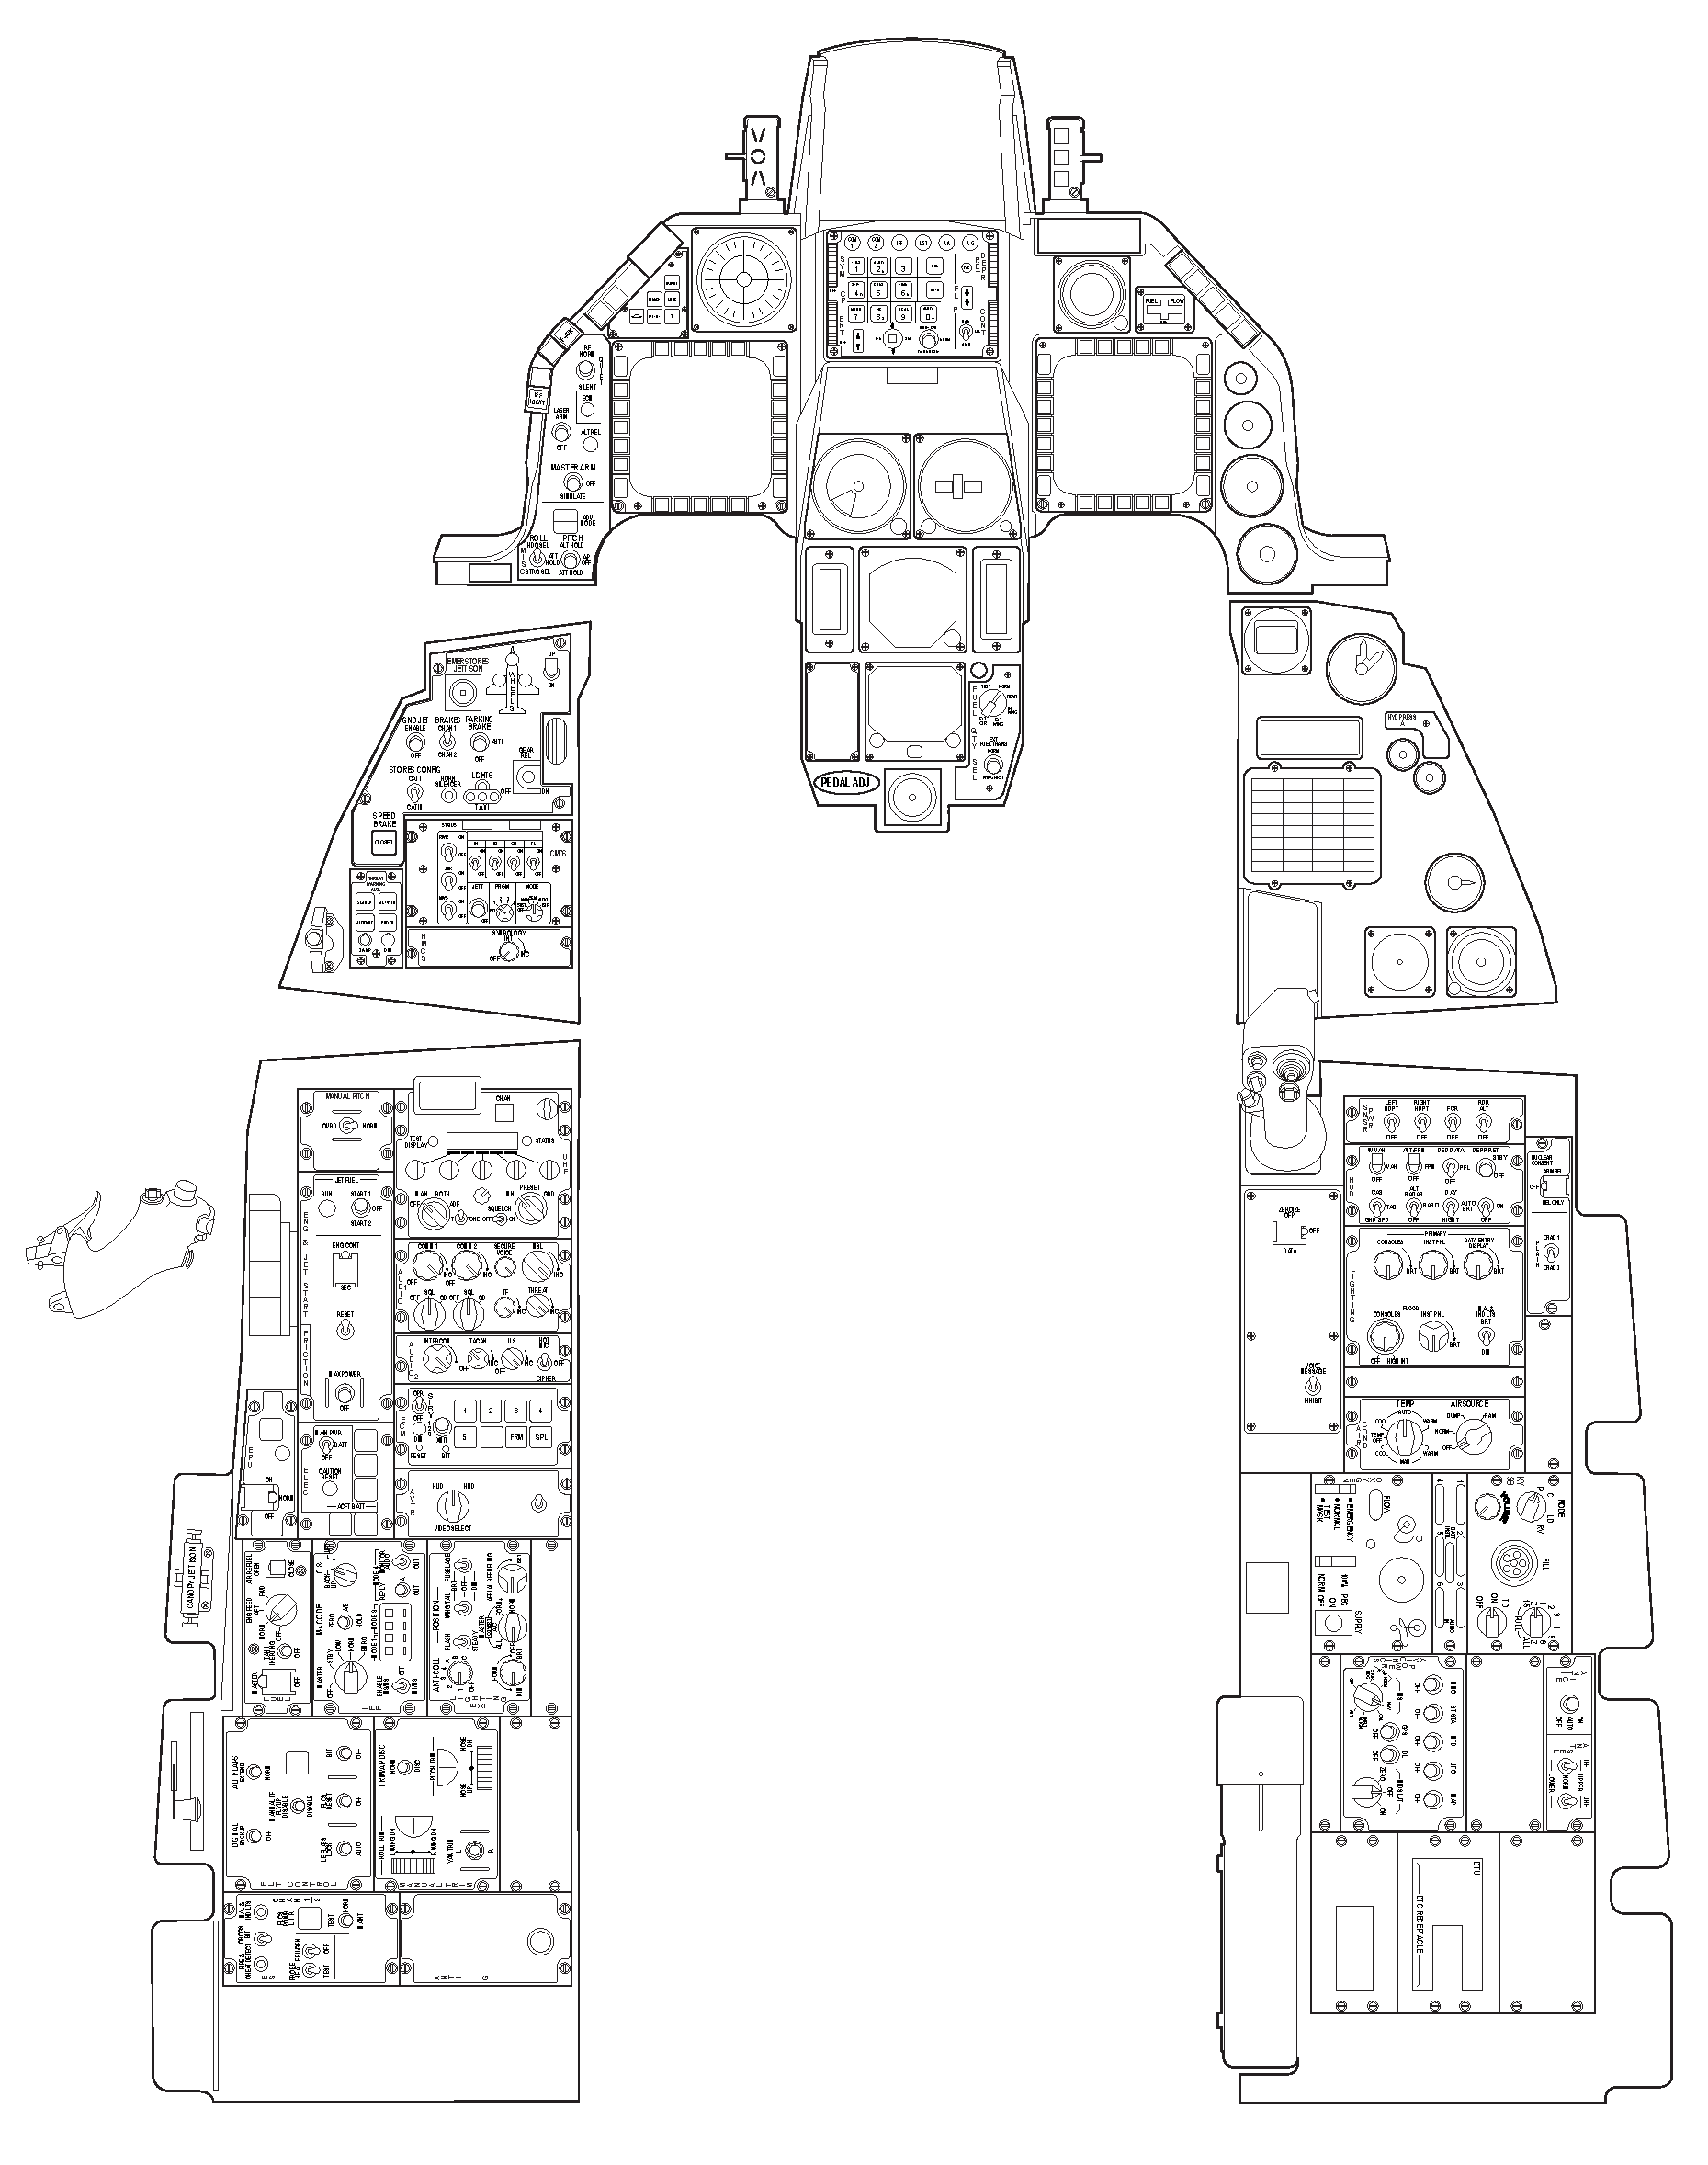
\includegraphics[
                height = 0.65\textheight
            ]{diagrams/cockpit/cockpit_full.pdf}
        };

        \draw[red] 
        (-2,58) -- ++(0,5) node [font=\footnotesize, left, pos=0.5] {10$^\circ$}
        (-10,49) -- ++(0,5) node [font=\footnotesize, left, pos=0.5] {20$^\circ$}
        (-18,42) -- ++(0,5) node [font=\footnotesize, left, pos=0.5] {30$^\circ$};

        \draw[color2] 
        (10,57) -- ++(5,0) node [font=\footnotesize, right, pos=1] {0$^\circ$}
        (18,48.5) -- ++(5,0) node [font=\footnotesize, right, pos=1] {10$^\circ$}
        (25.5,36.75) -- ++(5,0) node [font=\footnotesize, right, pos=1] {20$^\circ$}
        (30.5,27) -- ++(5,0) node [font=\footnotesize, right, pos=1] {30$^\circ$};
    \end{tikzpicture}
    \caption{F-16C block 52 cockpit overview. 
    Note the additional annotation lines which indicate vertical and horizontal angle references}
    \label{fig:cockpitoverview}
\end{figure}

\clearpage

\section{FORMATION}
\label{sec:suppfig:form}

\subsection{ELEMENT}

\begin{tcoloritemize}
    \blueitem[Fighting Wing]
    \textbf{Easiest for wingman} --- used in low-threat areas

    \medskip

    \textbf{Advantages}
    \begin{itemize}
        \item easy to maintain
        \item leader's 6'o'clock covered
        \item allows heads-down time
    \end{itemize}

    \textbf{Disadvantages}
    \begin{itemize}
        \item wingman's 6'o'clock NOT covered
        \item close proximity
    \end{itemize}

    Reference \cref{fig:supp_fig:form:fightingwing} for illustration
    \blueitem[Wedge]
    \textbf{Similar to fighting wing} --- more spaced out
    
    \medskip

    \textbf{Advantages}
    \begin{itemize}
        \item easy to maintain
        \item leader's 6'o'clock covered
        \item free for aggressive maneuvering
    \end{itemize}

    \textbf{Disadvantages}
    \begin{itemize}
        \item wingman's 6'o'clock NOT covered
        \item lead changes difficult
    \end{itemize}

    Reference \cref{fig:supp_fig:form:wedge} for illustration
\end{tcoloritemize}

\begin{figure}[htbp]
    \centering
    \begin{minipage}[b]{0.5\textwidth}
        \centering
        \begin{tikzpicture}[figstyle]
            
            \coordinate (lead) at (0,0);
            \coordinate (wing) at ($(lead)+(-45:27.5)$);
    
            \draw[dashed]
            (lead) -- ++(-30:15) arc (-30:-60:15) -- (lead);
    
            \draw[fill=color2!15]
            ($(lead)+(-30:15)$) 
            -- ++(-30:25) node[font=\footnotesize, pos=1, right] {30$^\circ$}
            arc  (-30:-60:40) 
            node[font=\footnotesize, below, pos=0.5, rotate=45] {0.5nm}
            node[font=\footnotesize, pos=1, below right] {60$^\circ$}
            -- ++(120:25)
            arc (-60:-30:15)
            node[font=\footnotesize, below, pos=0.5, rotate=45] {0.1nm};
    
            \node[yshift=-3mm] (leadfig) at (lead) {
                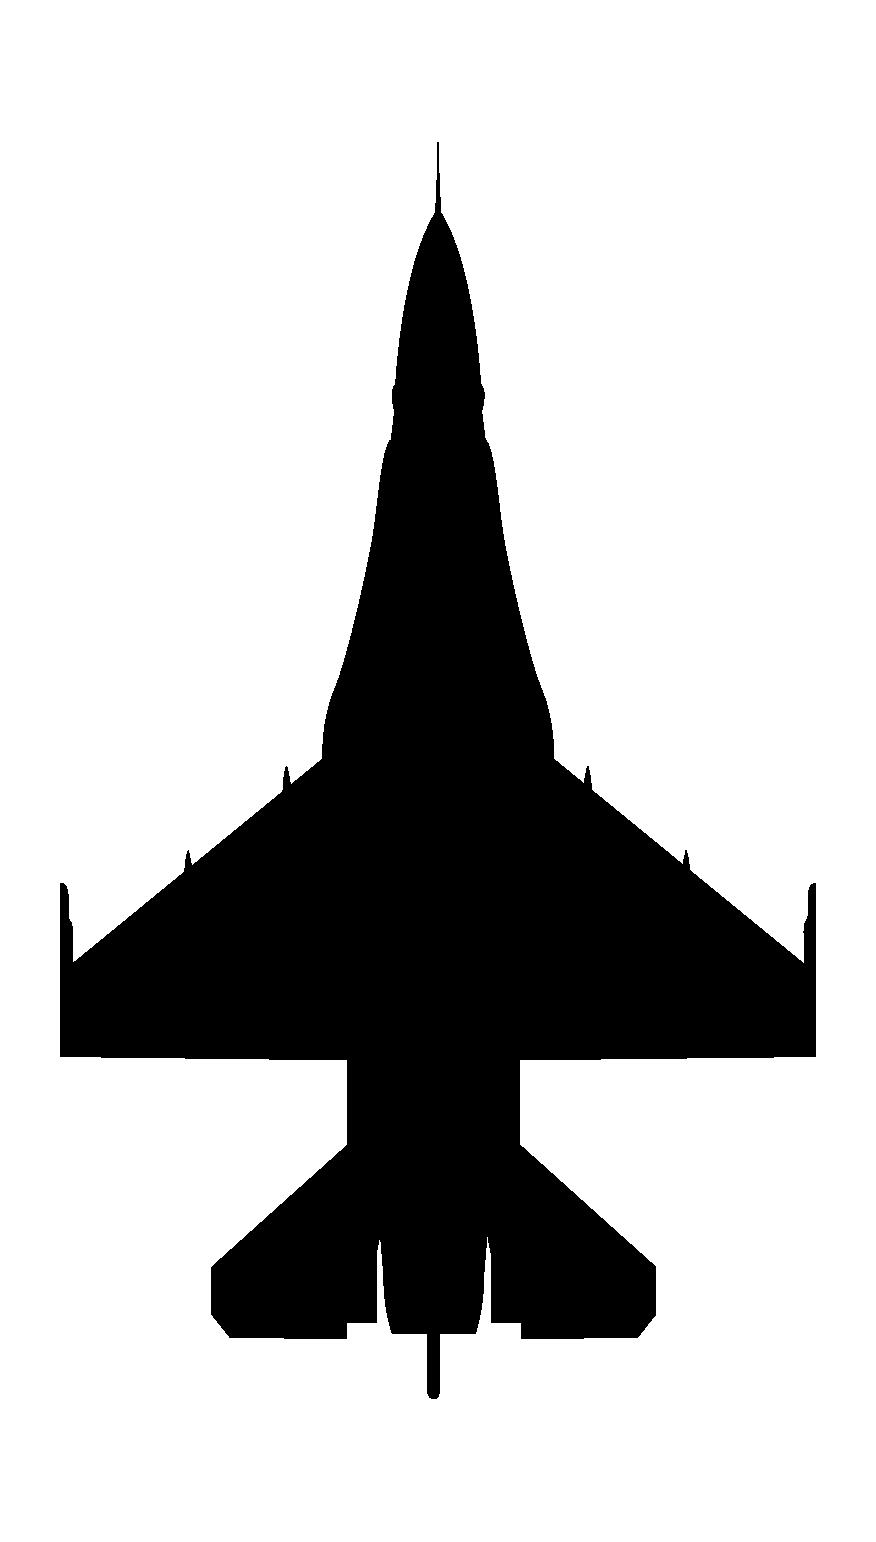
\includegraphics[
                    width=7.5mm,
                ]{diagrams/aircraft/silhouette_f16_top.pdf}
            };
            
            \node[] (wingfig) at (wing) {
                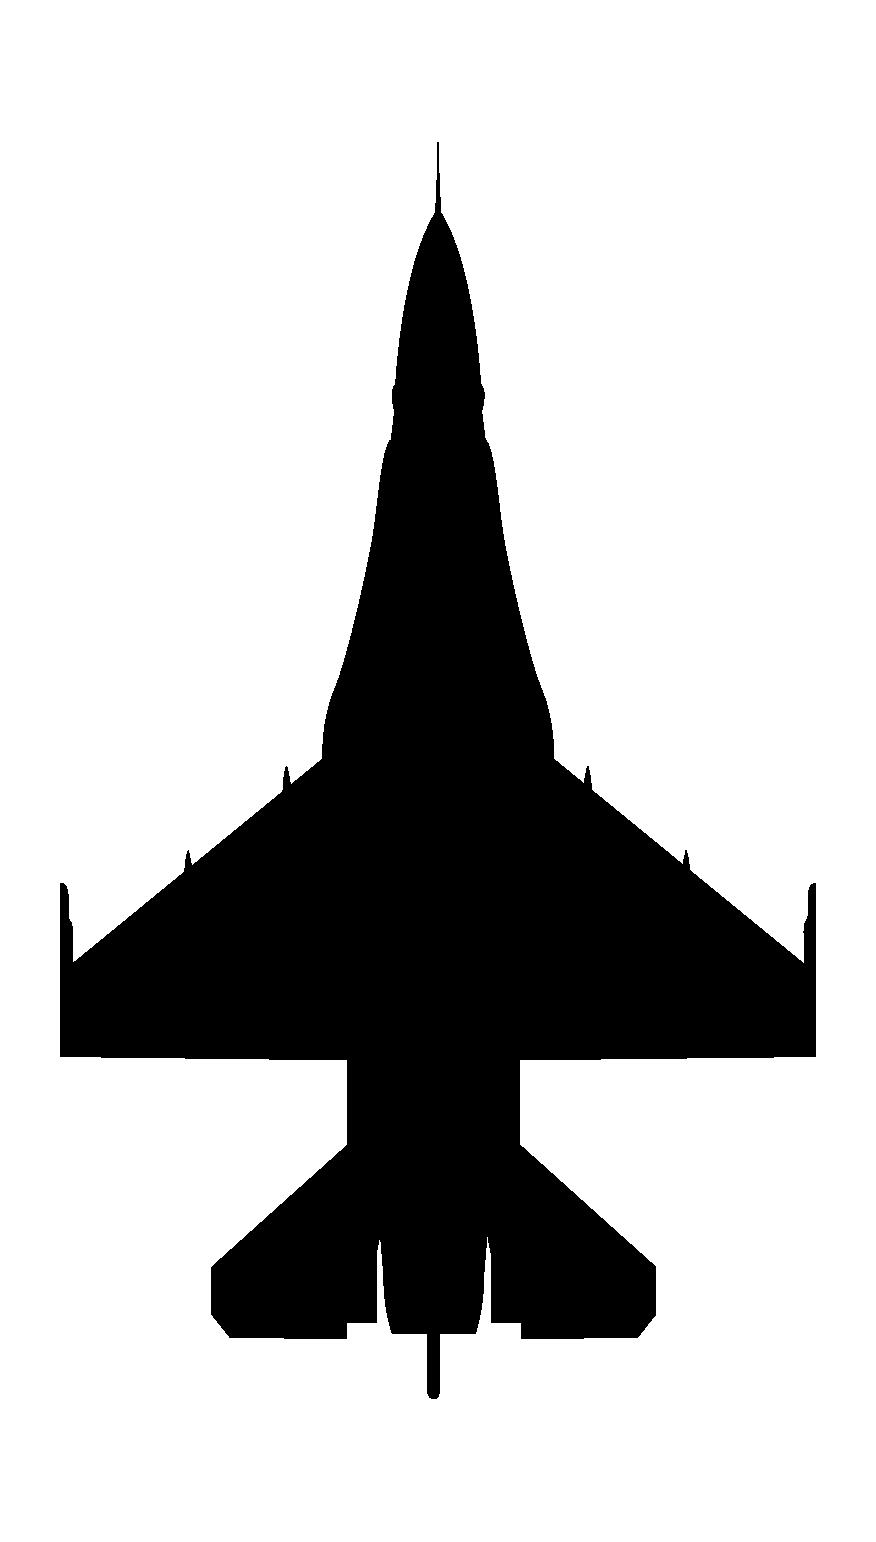
\includegraphics[
                    width=7.5mm,
                ]{diagrams/aircraft/silhouette_f16_top.pdf}
            };
    
        \end{tikzpicture}
        \caption{Fighting wing formation}
        \label{fig:supp_fig:form:fightingwing}
    \end{minipage}%
    \begin{minipage}[b]{0.5\textwidth}
        \centering
        \begin{tikzpicture}[figstyle]
            
            \coordinate (lead) at (0,0);
            \coordinate (wing) at ($(lead)+(-45:30)$);
    
            \draw[dashed]
            (lead) -- ++(-30:20) arc (-30:-60:20) -- (lead);
    
            \draw[fill=color2!15]
            ($(lead)+(-30:20)$) 
            -- ++(-30:20) node[font=\footnotesize, pos=1, right] {30$^\circ$}
            arc  (-30:-60:40) 
            node[font=\footnotesize, below, pos=0.5, rotate=45] {1.0 nm}
            node[font=\footnotesize, pos=1, below right] {60$^\circ$}
            -- ++(120:20)
            arc (-60:-30:20)
            node[font=\footnotesize, below, pos=0.5, rotate=45] {0.5 nm};
    
            \node[yshift=-3mm] (leadfig) at (lead) {
                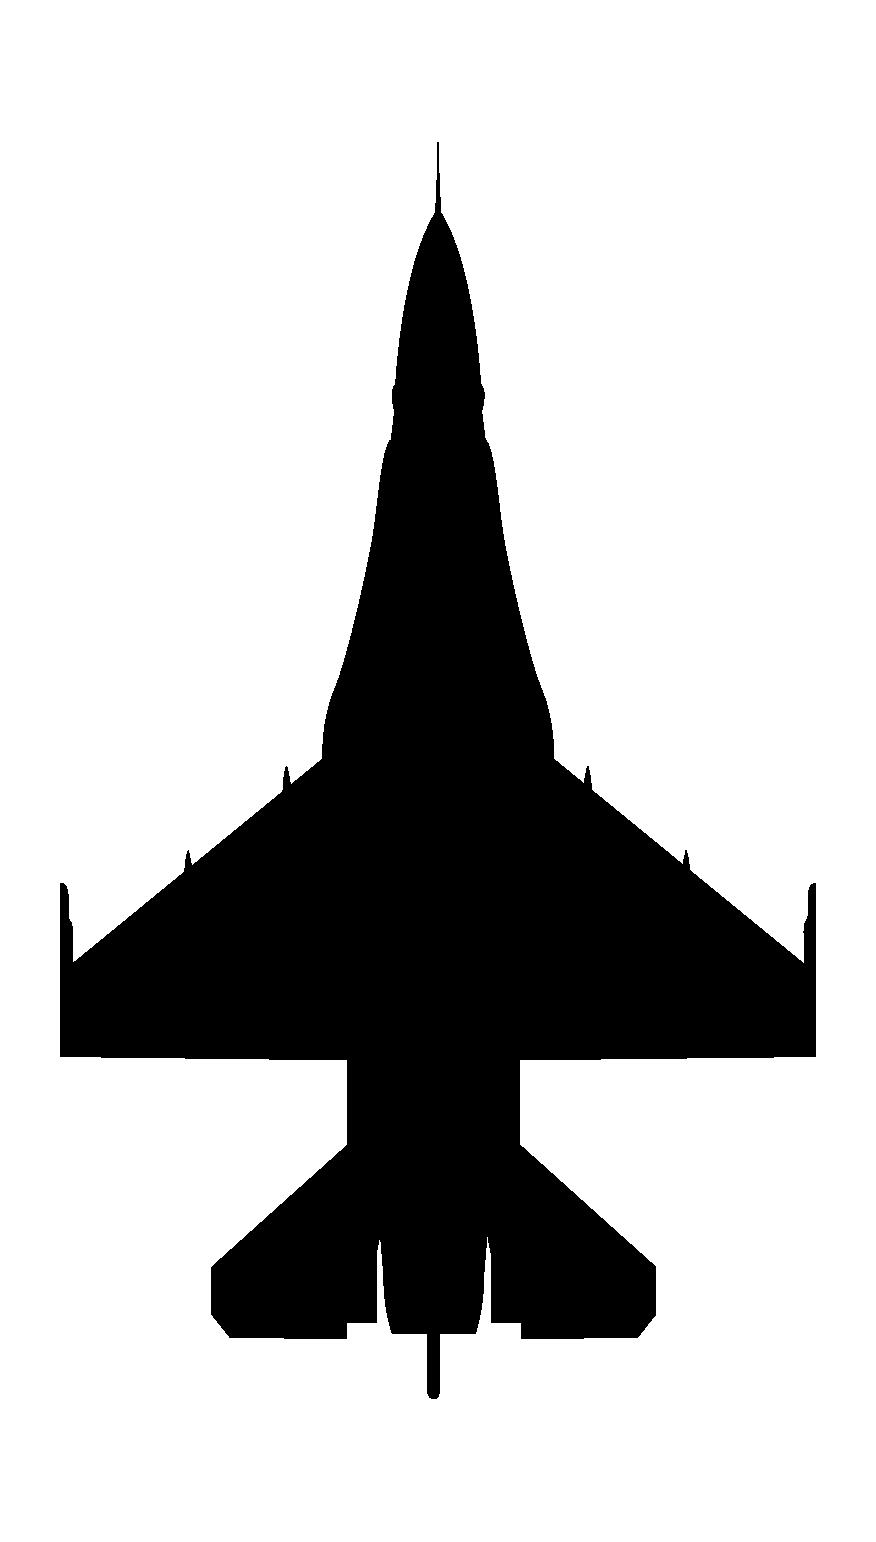
\includegraphics[
                    width=7.5mm,
                ]{diagrams/aircraft/silhouette_f16_top.pdf}
            };
            
            \node[] (wingfig) at (wing) {
                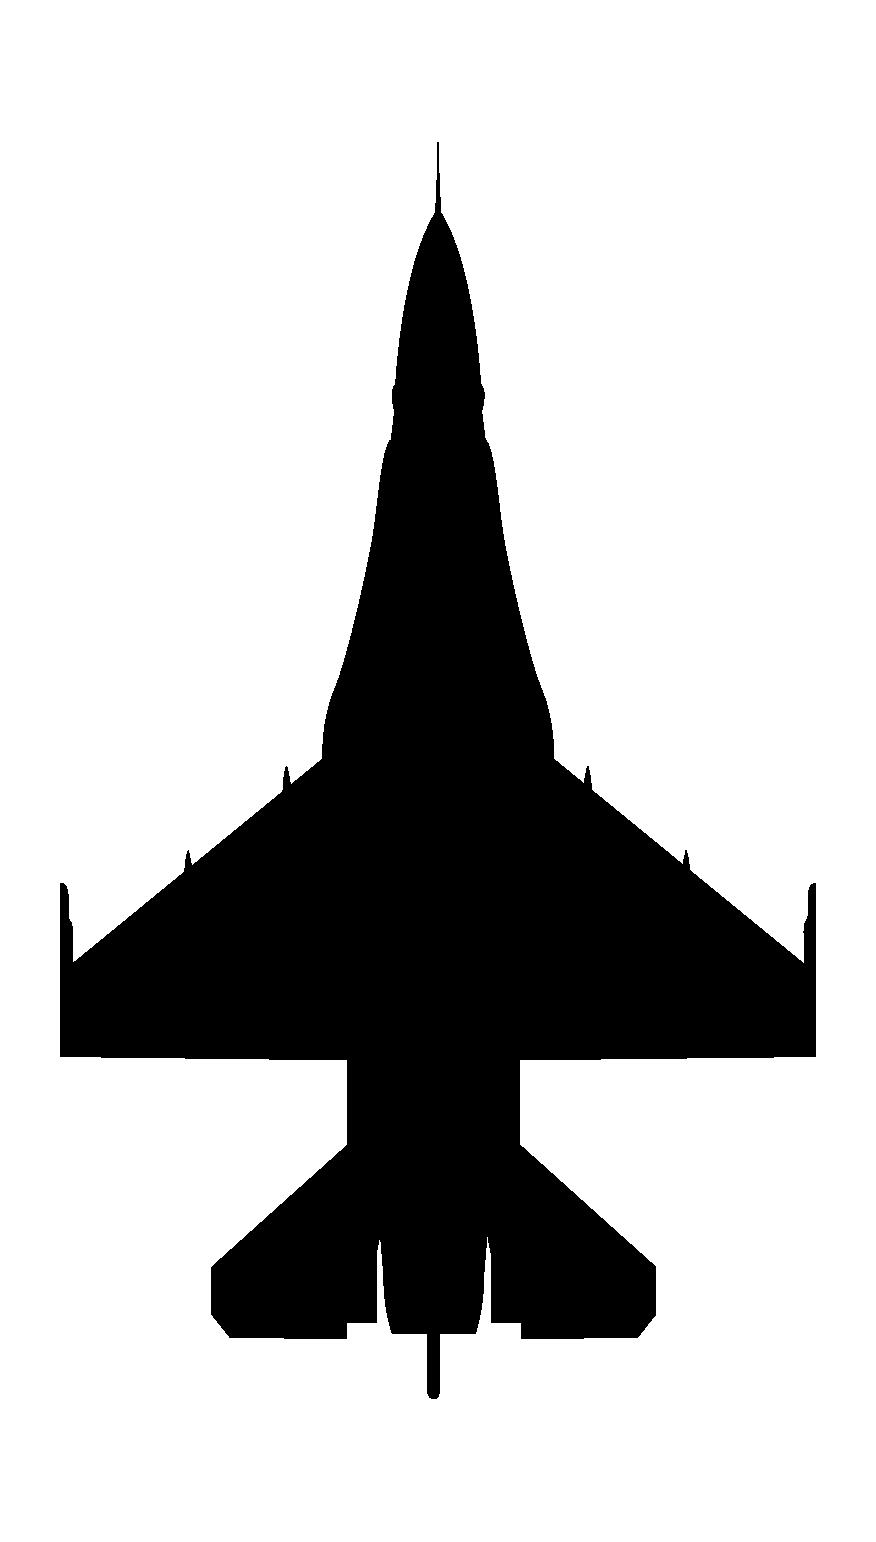
\includegraphics[
                    width=7.5mm,
                ]{diagrams/aircraft/silhouette_f16_top.pdf}
            };
    
        \end{tikzpicture}
        \caption{Two-ship wedge formation}
        \label{fig:supp_fig:form:wedge}
    \end{minipage}
\end{figure}

\begin{tcoloritemize}
    \blueitem[Line Abreast]
    \textbf{Tactical A-A Formation} --- mutual 6'o'clock cover, ensures all flight members in position to shoot simultaneously
    \medskip

    \textbf{Advantages}
    \begin{itemize}
        \item mutual 6'o'clock cover
        \item laterally spread
        \item simplifies tactical turns
        \item allows simultaneous bandit engagement
    \end{itemize}

    \textbf{Disadvantages}
    \begin{itemize}
        \item difficult to maintain
    \end{itemize}

    Reference \cref{fig:supp_fig:form:lineabreast} for illustration

    \blueitem[Spread]
    \textbf{Similar to line abreast} --- more room for wingman to maneuver

    Reference \cref{fig:supp_fig:form:lineabreast} for illustration
\end{tcoloritemize}


\begin{figure}[htbp]
    \centering
    \begin{minipage}[b]{0.55\textwidth}
        \centering
        \begin{tikzpicture}[figstyle]
        
            \coordinate (lead) at (0,0);
            \coordinate (wing) at ($(lead)+(0:40)$);
    
            \draw[dashed]
            (lead) -- ++(0:20) arc (0:-20:20) -- (lead);
    
            \draw[fill=color2!15]
            ($(lead)+(0:20)$) 
            -- ++(0:40) node[font=\footnotesize, pos=1, right] {0$^\circ$}
            arc  (0:-20:60) 
            node[font=\footnotesize, right, pos=0.5] {2.0 nm}
            node[font=\footnotesize, pos=1, below right] {20$^\circ$}
            -- ++(160:40)
            arc (-20:0:20)
            node[font=\footnotesize, right, pos=0.5] {0.7 nm};
    
            \node[yshift=-3mm] (leadfig) at (lead) {
                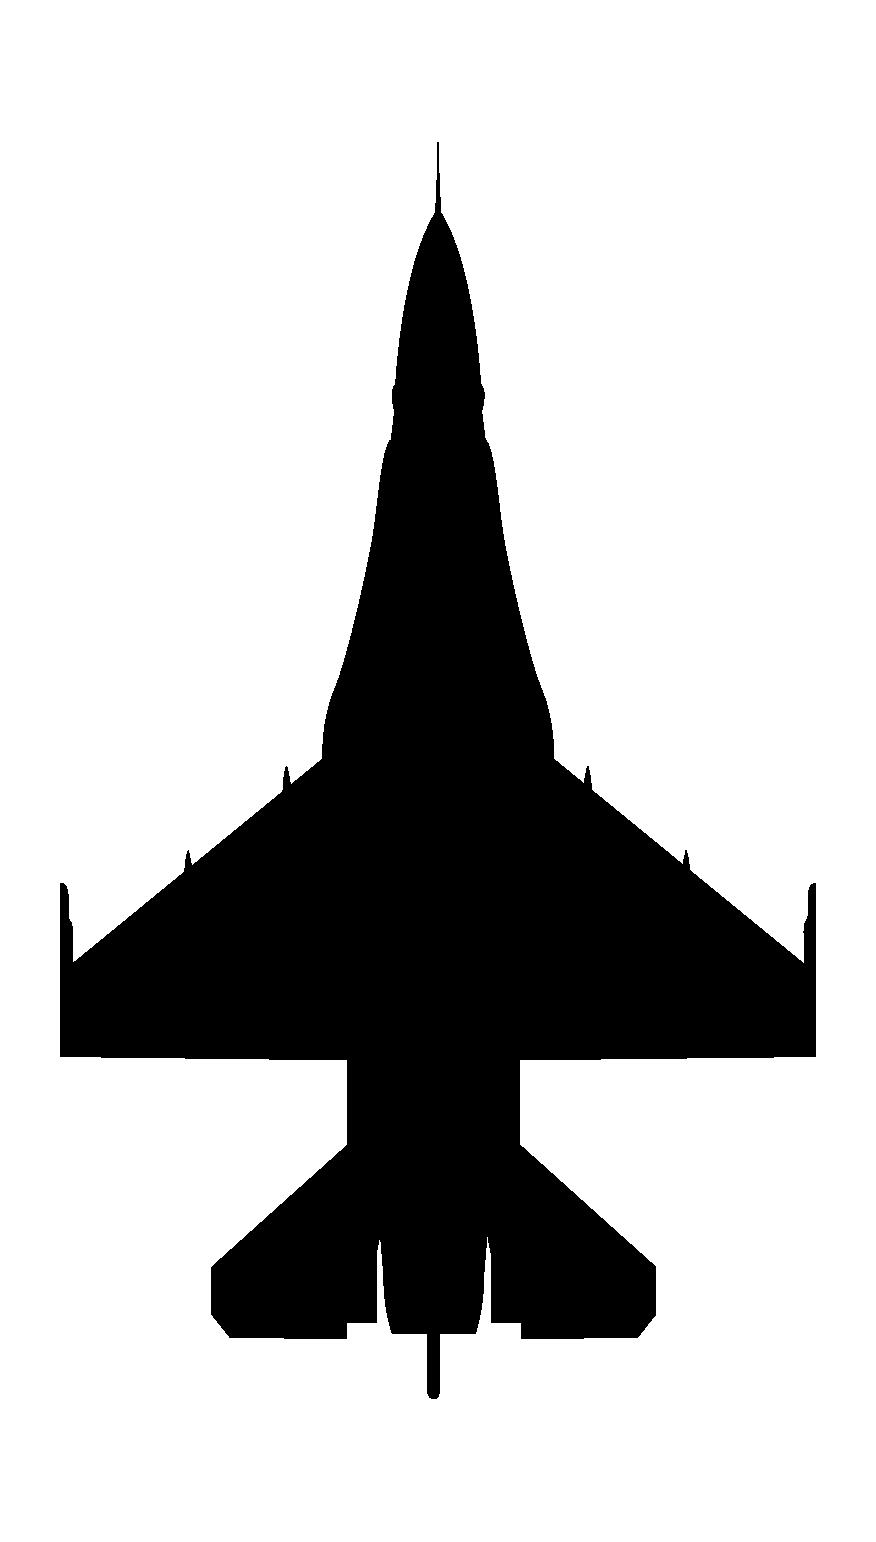
\includegraphics[
                    width=7.5mm,
                ]{diagrams/aircraft/silhouette_f16_top.pdf}
            };
            
            \node[yshift=-3mm] (wingfig) at (wing) {
                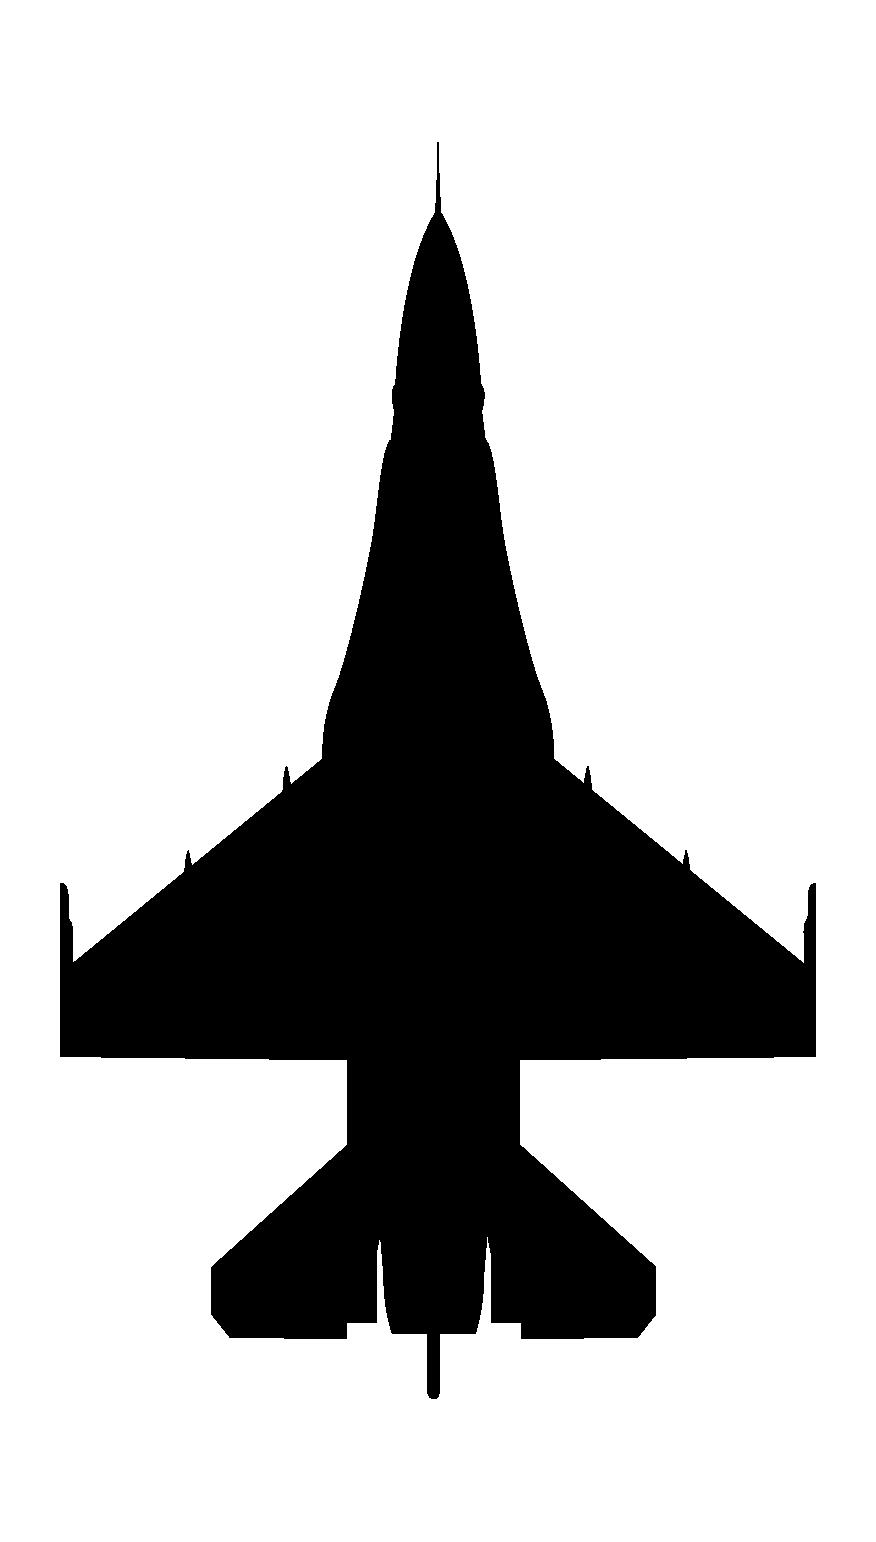
\includegraphics[
                    width=7.5mm,
                ]{diagrams/aircraft/silhouette_f16_top.pdf}
            };
    
        \end{tikzpicture}
        \caption{Two-ship line abreast formation}
        \label{fig:supp_fig:form:lineabreast}
    \end{minipage}%
    \begin{minipage}[b]{0.45\textwidth}
        \centering
        \begin{tikzpicture}[figstyle]
        
            \coordinate (lead) at (0,0);
            \coordinate (wing) at ($(lead)+(-30:30)$);
    
            \draw[dashed]
            (lead) -- ++(0:20) arc (0:-60:20) -- (lead);
    
            \draw[fill=color2!15]
            ($(lead)+(0:20)$) 
            -- ++(0:20) node[font=\footnotesize, pos=1, right] {0$^\circ$}
            arc  (0:-60:40) 
            node[font=\footnotesize, right, pos=0.5] {2.0 nm}
            node[font=\footnotesize, pos=1, below right] {60$^\circ$}
            -- ++(120:20)
            arc (-60:0:20)
            node[font=\footnotesize, right, pos=0.75] {1.0 nm};
    
            \node[yshift=-3mm] (leadfig) at (lead) {
                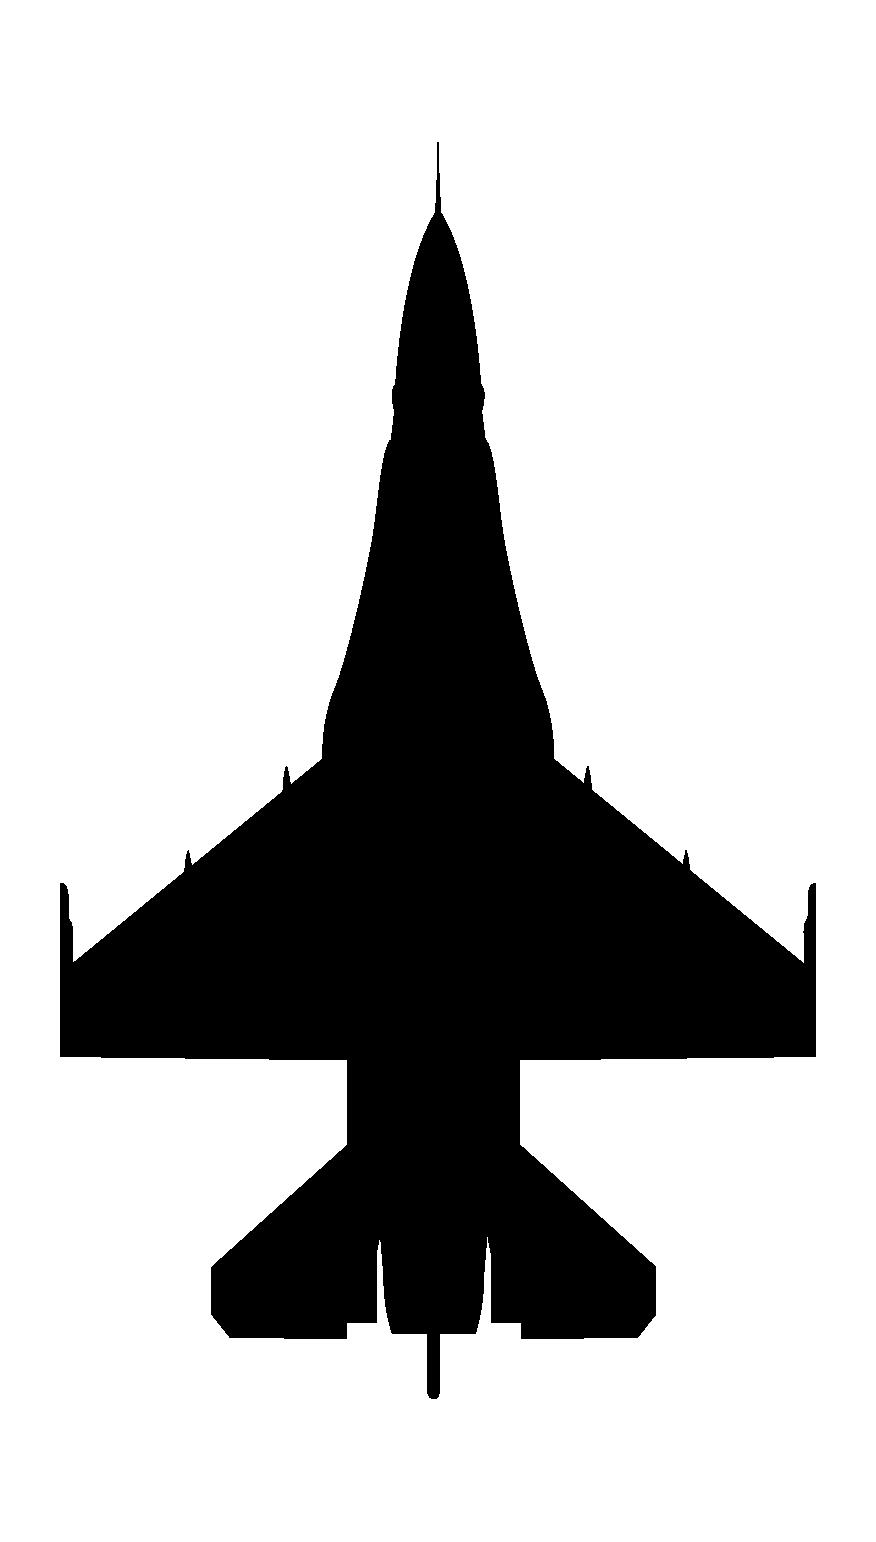
\includegraphics[
                    width=7.5mm,
                ]{diagrams/aircraft/silhouette_f16_top.pdf}
            };
            
            \node[yshift=-0mm] (wingfig) at (wing) {
                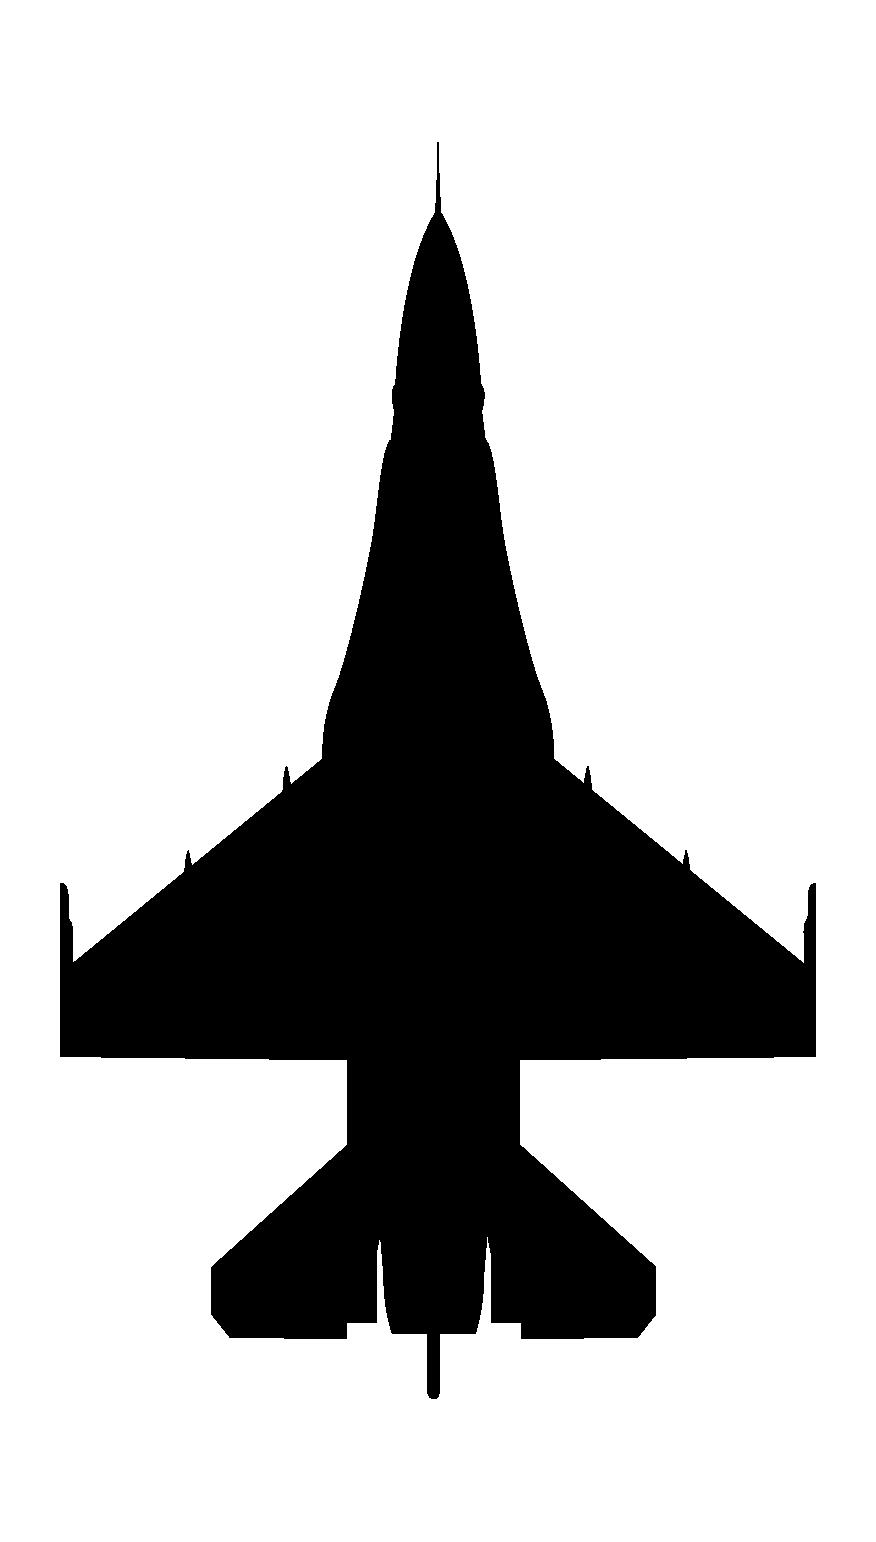
\includegraphics[
                    width=7.5mm,
                ]{diagrams/aircraft/silhouette_f16_top.pdf}
            };
    
        \end{tikzpicture}
        \caption{Two-ship spread formation}
        \label{fig:supp_fig:form:spread}
    \end{minipage}
\end{figure}

\clearpage

\subsection{FOUR-SHIP}

\begin{figure}[htbp]
    \centering
    \begin{minipage}[b]{0.5\textwidth}
        \centering
        \begin{tikzpicture}[figstyle]
            
            \coordinate (1) at (0,0);
            \coordinate (2) at ($(1)+(20,0)$);
            \coordinate (3) at ($(1)+(0,-30)$);
            \coordinate (4) at ($(3)+(20,0)$);

            \draw[thin, <->]
            ($(1)+(-5,0)$) 
            -- ($(3)+(-5,0)$)
            node[font=\footnotesize, pos=0.5, rotate=90, above] {1.5-3.0 nm};
            \draw[thin]
            (1) -- ($(1)+(-7,0)$)
            (3) -- ($(3)+(-7,0)$);

            \draw[thin, <->]
            ($(1)+(0,5)$) 
            -- ($(2)+(0,5)$)
            node[font=\footnotesize, pos=0.5, above] {line abreast};
            \draw[thin]
            (1) -- ($(1)+(0,7)$)
            (2) -- ($(2)+(0,7)$);

            \draw[thin, <->]
            ($(3)+(0,5)$) 
            -- ($(4)+(0,5)$)
            node[font=\footnotesize, pos=0.5, above] {line abreast};
            \draw[thin]
            (3) -- ($(3)+(0,7)$)
            (4) -- ($(4)+(0,7)$);


            \node[yshift=-2mm] (1fig) at (1) {
                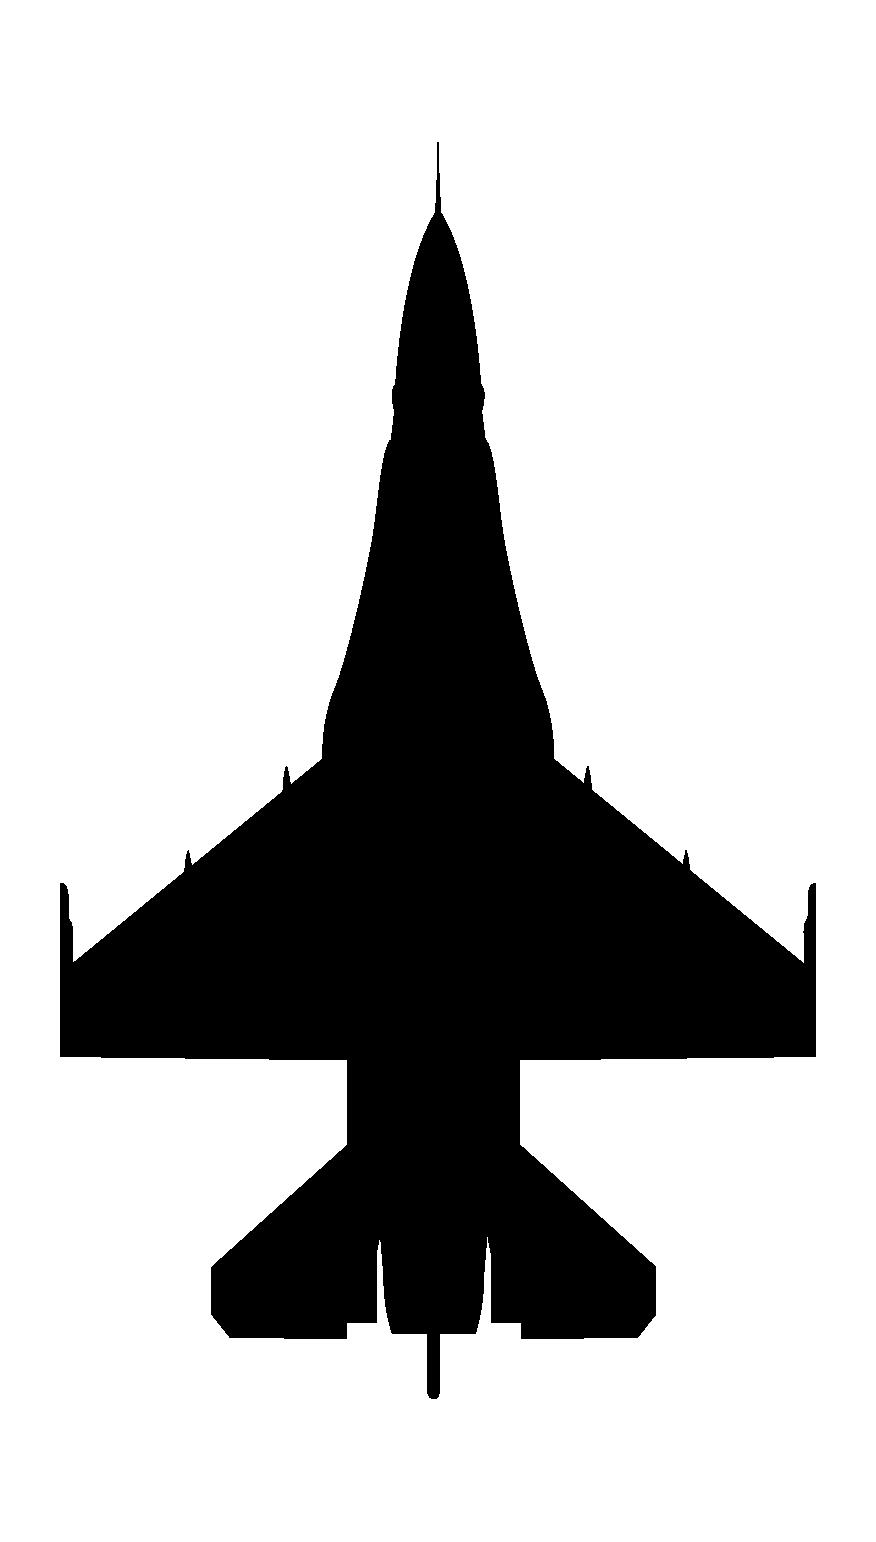
\includegraphics[
                    width=7.5mm,
                ]{diagrams/aircraft/silhouette_f16_top.pdf}
            };
            
            \node[yshift=-2mm] (2fig) at (2) {
                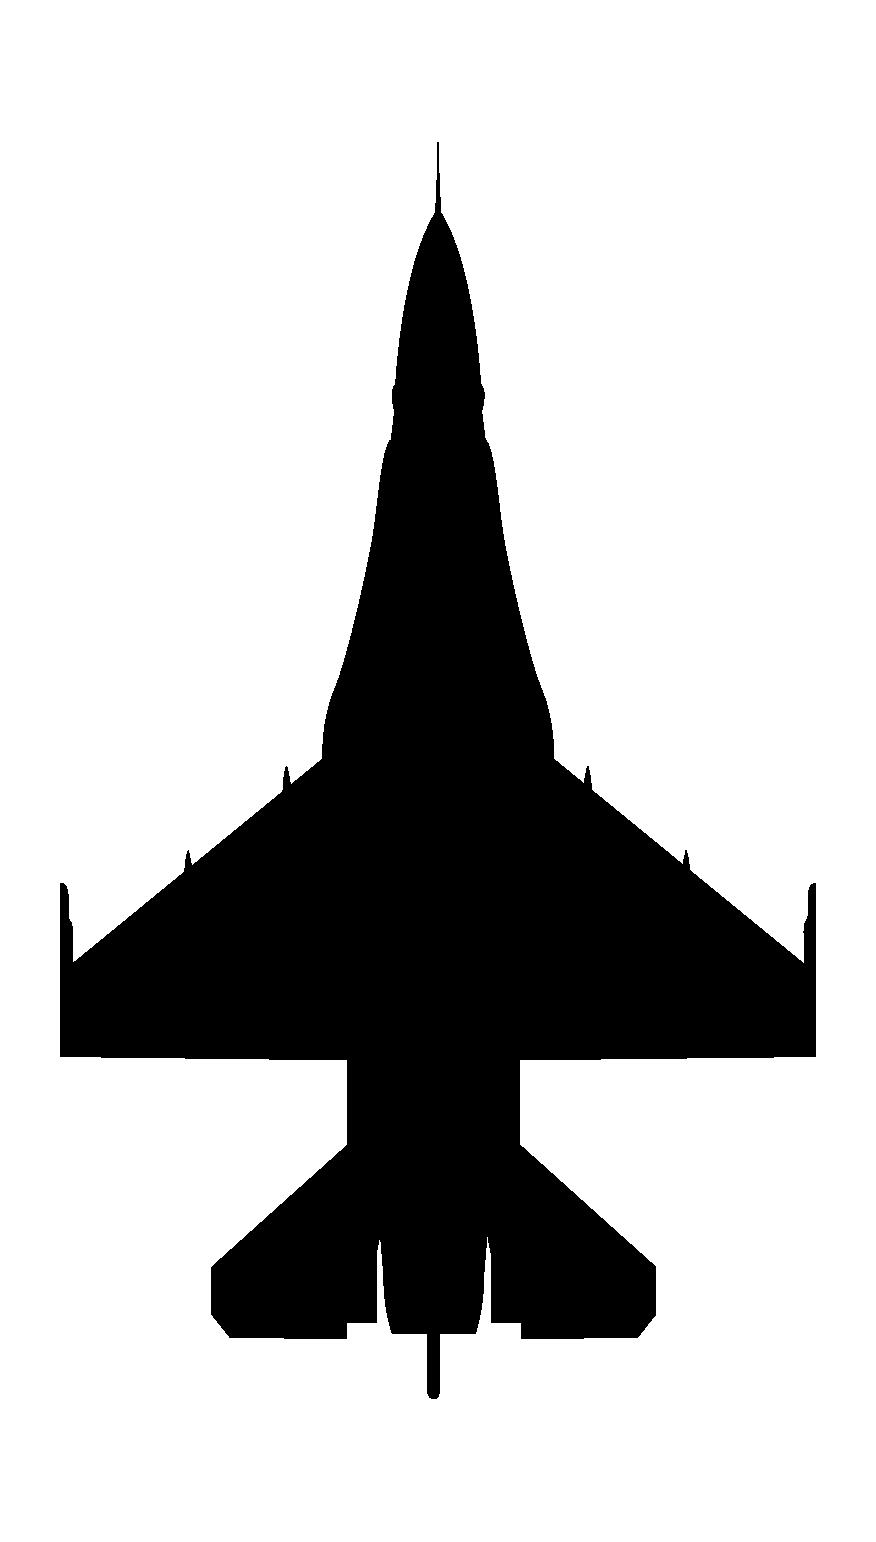
\includegraphics[
                    width=7.5mm,
                ]{diagrams/aircraft/silhouette_f16_top.pdf}
            };

            \node[yshift=-2mm] (3fig) at (3) {
                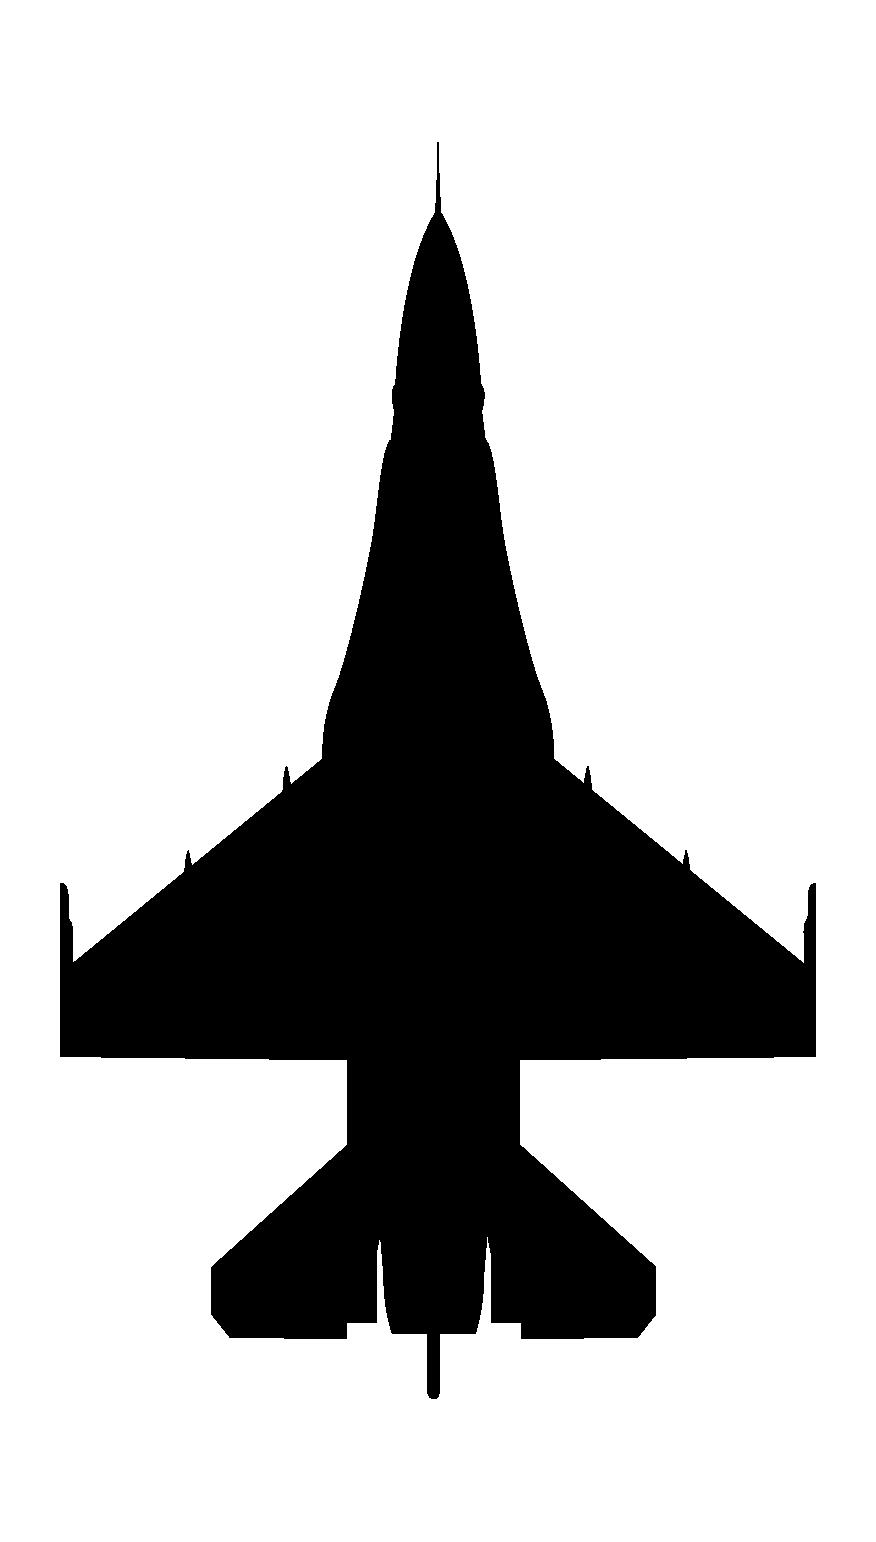
\includegraphics[
                    width=7.5mm,
                ]{diagrams/aircraft/silhouette_f16_top.pdf}
            };
            
            \node[yshift=-2mm] (4fig) at (4) {
                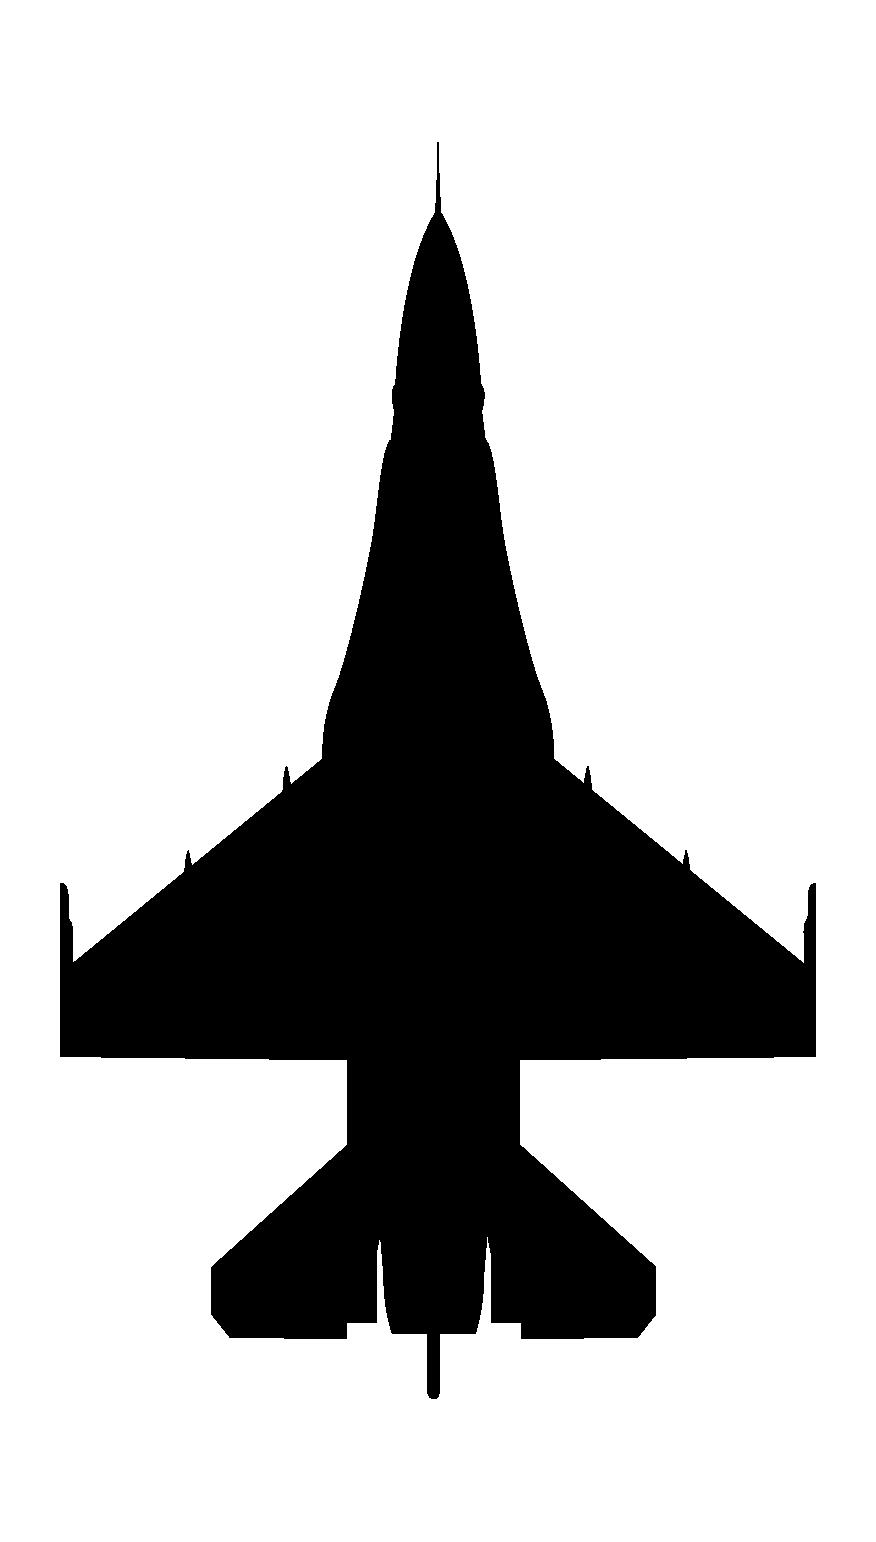
\includegraphics[
                    width=7.5mm,
                ]{diagrams/aircraft/silhouette_f16_top.pdf}
            };

            \node[anchor=north, font=\footnotesize] (1label) at (1fig.south) {1};
            \node[anchor=north, font=\footnotesize] (2label) at (2fig.south) {2};
            \node[anchor=north, font=\footnotesize] (3label) at (3fig.south) {3};
            \node[anchor=north, font=\footnotesize] (4label) at (4fig.south) {4};

        \end{tikzpicture}
        \caption{Four-ship box formation}
        \label{fig:supp_fig:form:box}
    \end{minipage}%
    \begin{minipage}[b]{0.5\textwidth}
        \centering
        \begin{tikzpicture}[figstyle]
            
            \coordinate (1) at (0,0);
            \coordinate (2) at ($(1)+(20,0)$);
            \coordinate (3) at ($(1)+(10,-30)$);
            \coordinate (4) at ($(3)+(20,0)$);

            \draw[thin, <->]
            ($(1)+(-5,0)$) 
            -- ($(3)+(-15,0)$)
            node[font=\footnotesize, pos=0.5, rotate=90, above] {1.5-3.0 nm};
            \draw[thin]
            (1) -- ($(1)+(-7,0)$)
            (3) -- ($(3)+(-17,0)$);

            \draw[thin, <->]
            ($(1)+(0,5)$) 
            -- ($(2)+(0,5)$)
            node[font=\footnotesize, pos=0.5, above] {line abreast};
            \draw[thin]
            (1) -- ($(1)+(0,7)$)
            (2) -- ($(2)+(0,7)$);

            \draw[thin, <->]
            ($(3)+(0,5)$) 
            -- ($(4)+(0,5)$)
            node[font=\footnotesize, pos=0.5, above] {line abreast};
            \draw[thin]
            (3) -- ($(3)+(0,7)$)
            (4) -- ($(4)+(0,7)$);


            \node[yshift=-2mm] (1fig) at (1) {
                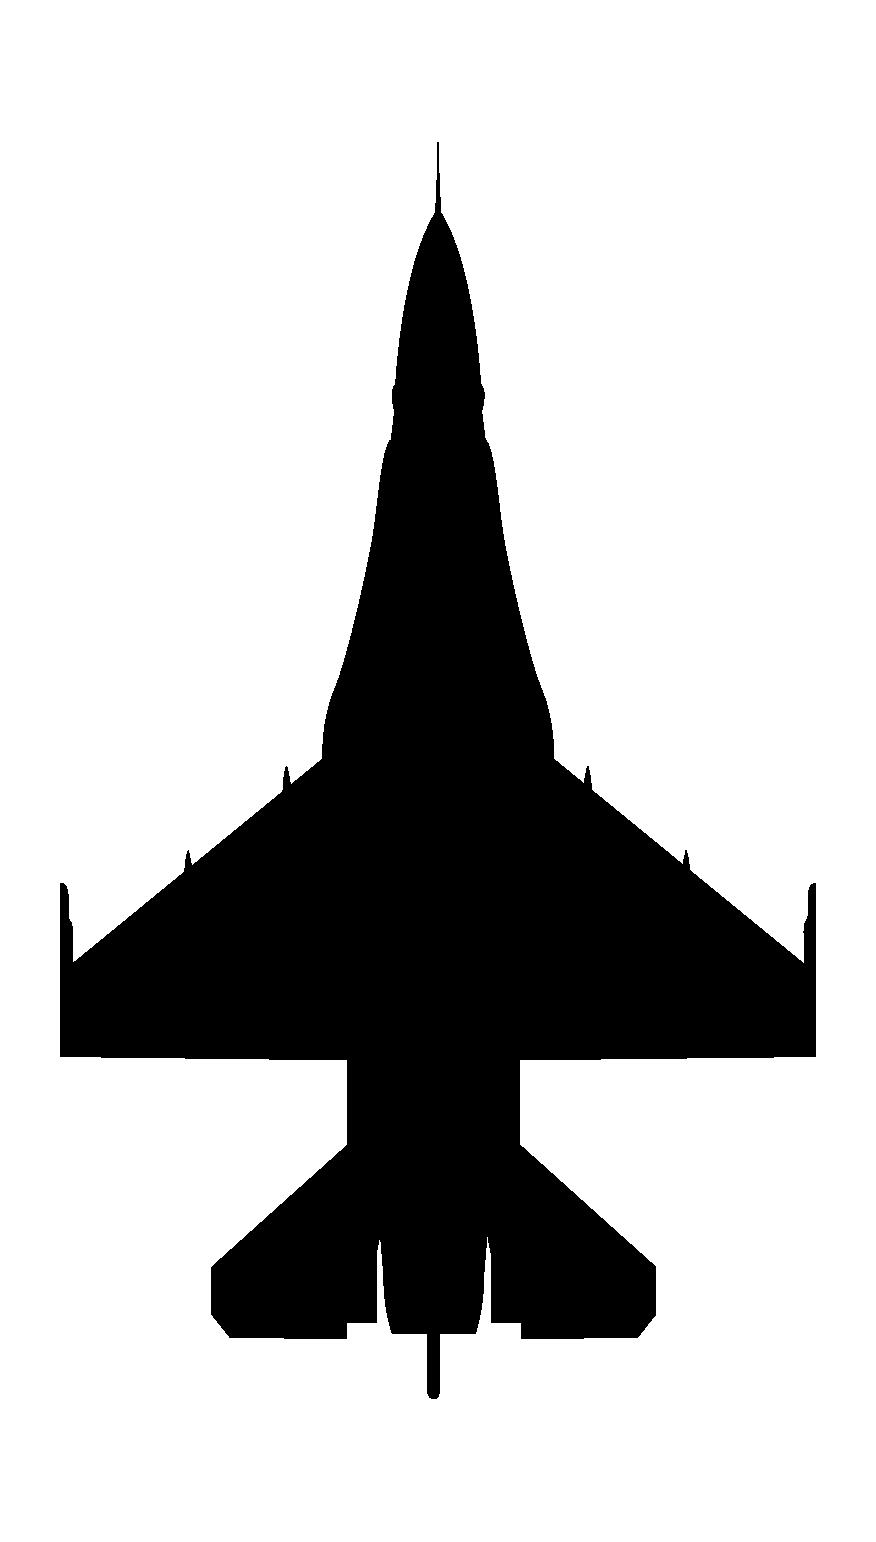
\includegraphics[
                    width=7.5mm,
                ]{diagrams/aircraft/silhouette_f16_top.pdf}
            };
            
            \node[yshift=-2mm] (2fig) at (2) {
                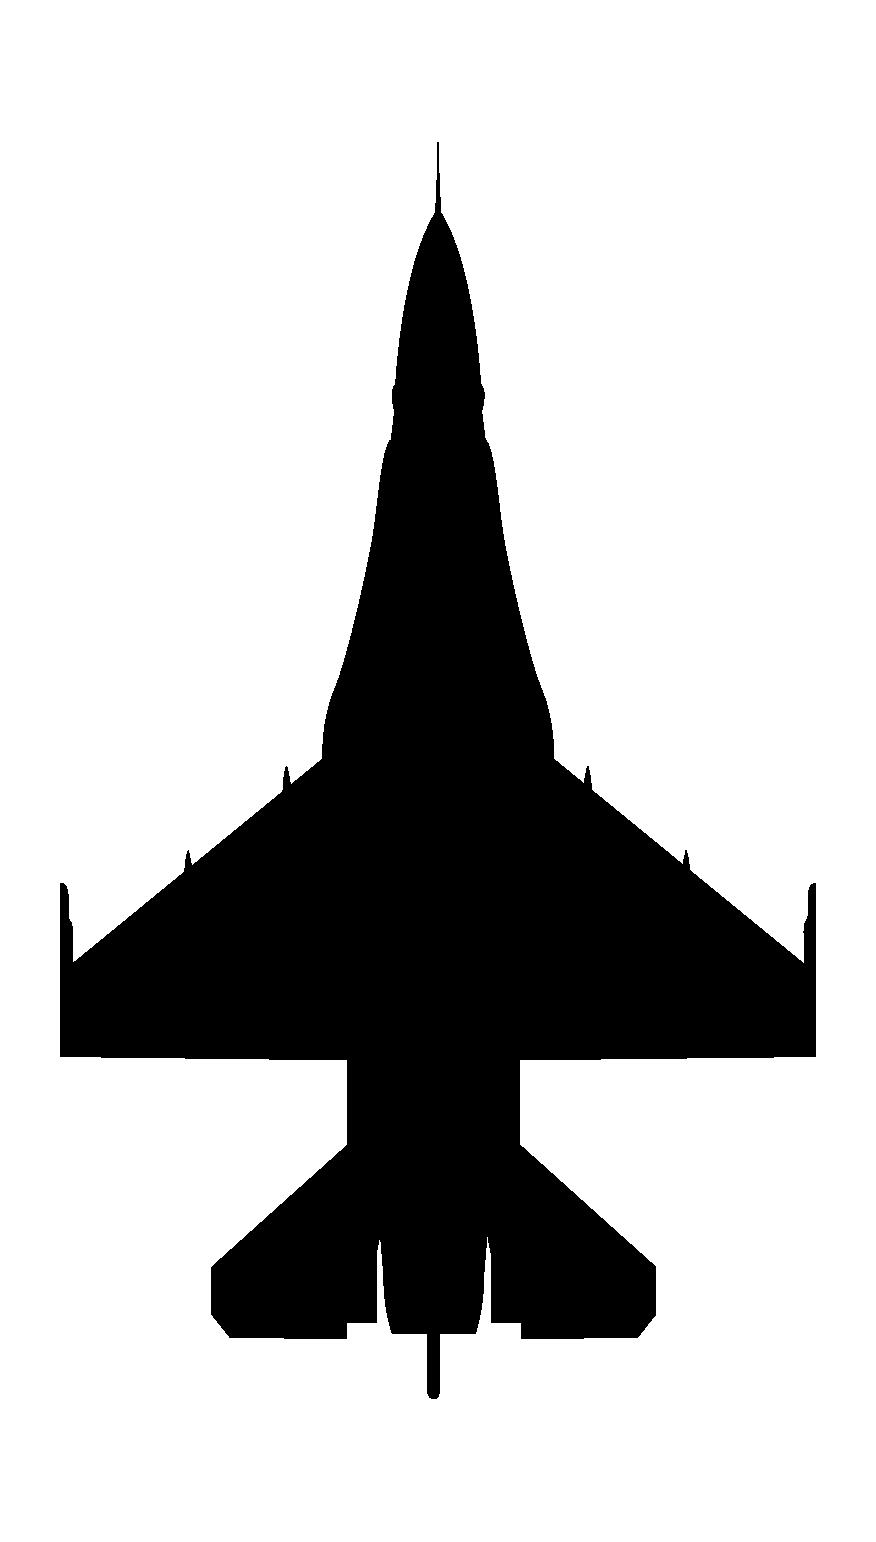
\includegraphics[
                    width=7.5mm,
                ]{diagrams/aircraft/silhouette_f16_top.pdf}
            };

            \node[yshift=-2mm] (3fig) at (3) {
                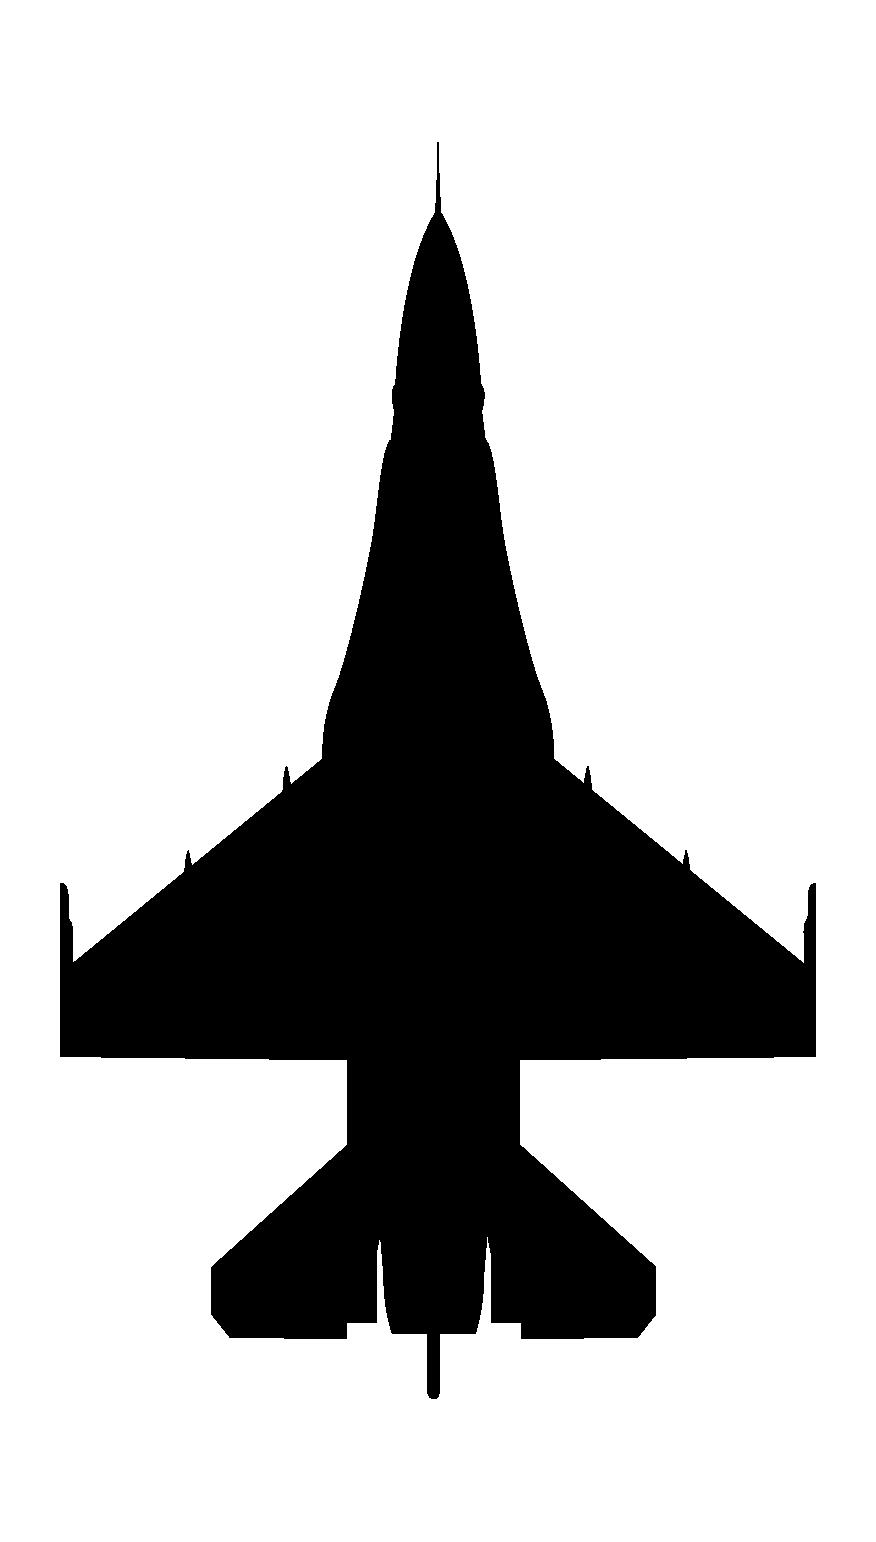
\includegraphics[
                    width=7.5mm,
                ]{diagrams/aircraft/silhouette_f16_top.pdf}
            };
            
            \node[yshift=-2mm] (4fig) at (4) {
                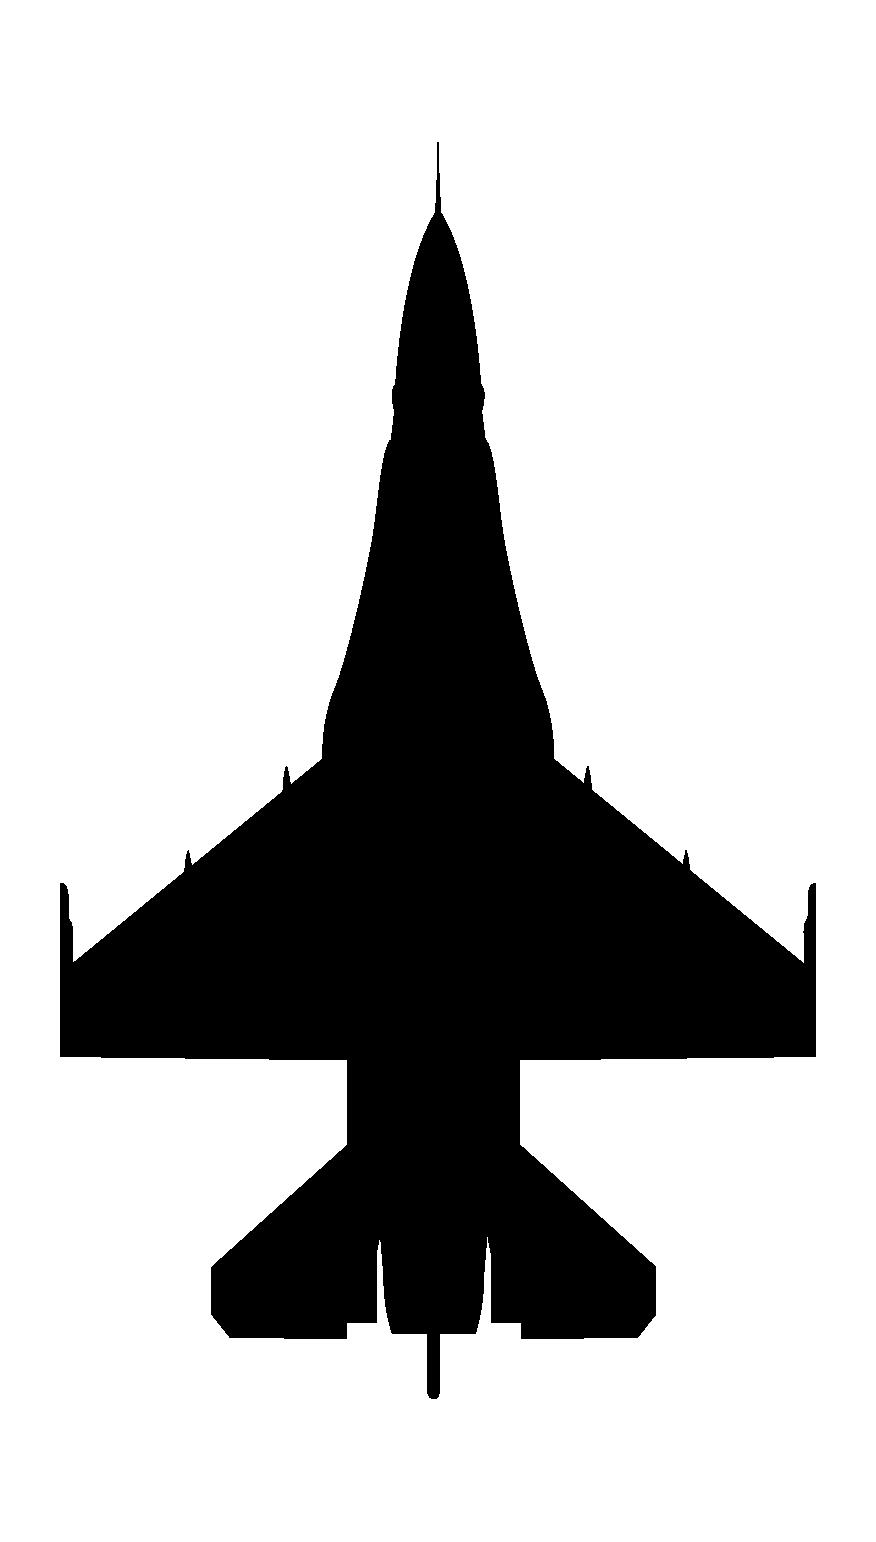
\includegraphics[
                    width=7.5mm,
                ]{diagrams/aircraft/silhouette_f16_top.pdf}
            };

            \node[anchor=north, font=\footnotesize] (1label) at (1fig.south) {1};
            \node[anchor=north, font=\footnotesize] (2label) at (2fig.south) {2};
            \node[anchor=north, font=\footnotesize] (3label) at (3fig.south) {3};
            \node[anchor=north, font=\footnotesize] (4label) at (4fig.south) {4};

        \end{tikzpicture}
        \caption{Four-ship offset box formation}
        \label{fig:supp_fig:form:boxoffset}
    \end{minipage}
\end{figure}

\begin{figure}[htbp]
    \centering
    \begin{tikzpicture}[figstyle]
        
        \coordinate (1) at (0,0);
        \coordinate (2) at ($(1)+(-135:20)$);
        \coordinate (3) at ($(1)+(20,0)$);
        \coordinate (4) at ($(3)+(-45:20)$);

        \draw[thin]
        (1) -- (2) node[font=\footnotesize, pos=0.5, above left] {fighting wing}
        (3) -- (4)node[font=\footnotesize, pos=0.5, above right] {fighting wing};

        \draw[thin, <->]
        ($(1)+(0,5)$) 
        -- ($(3)+(0,5)$)
        node[font=\footnotesize, pos=0.5, above] {line abreast};
        \draw[thin]
        (1) -- ($(1)+(0,7)$)
        (3) -- ($(3)+(0,7)$);

        \node[yshift=-2mm] (1fig) at (1) {
            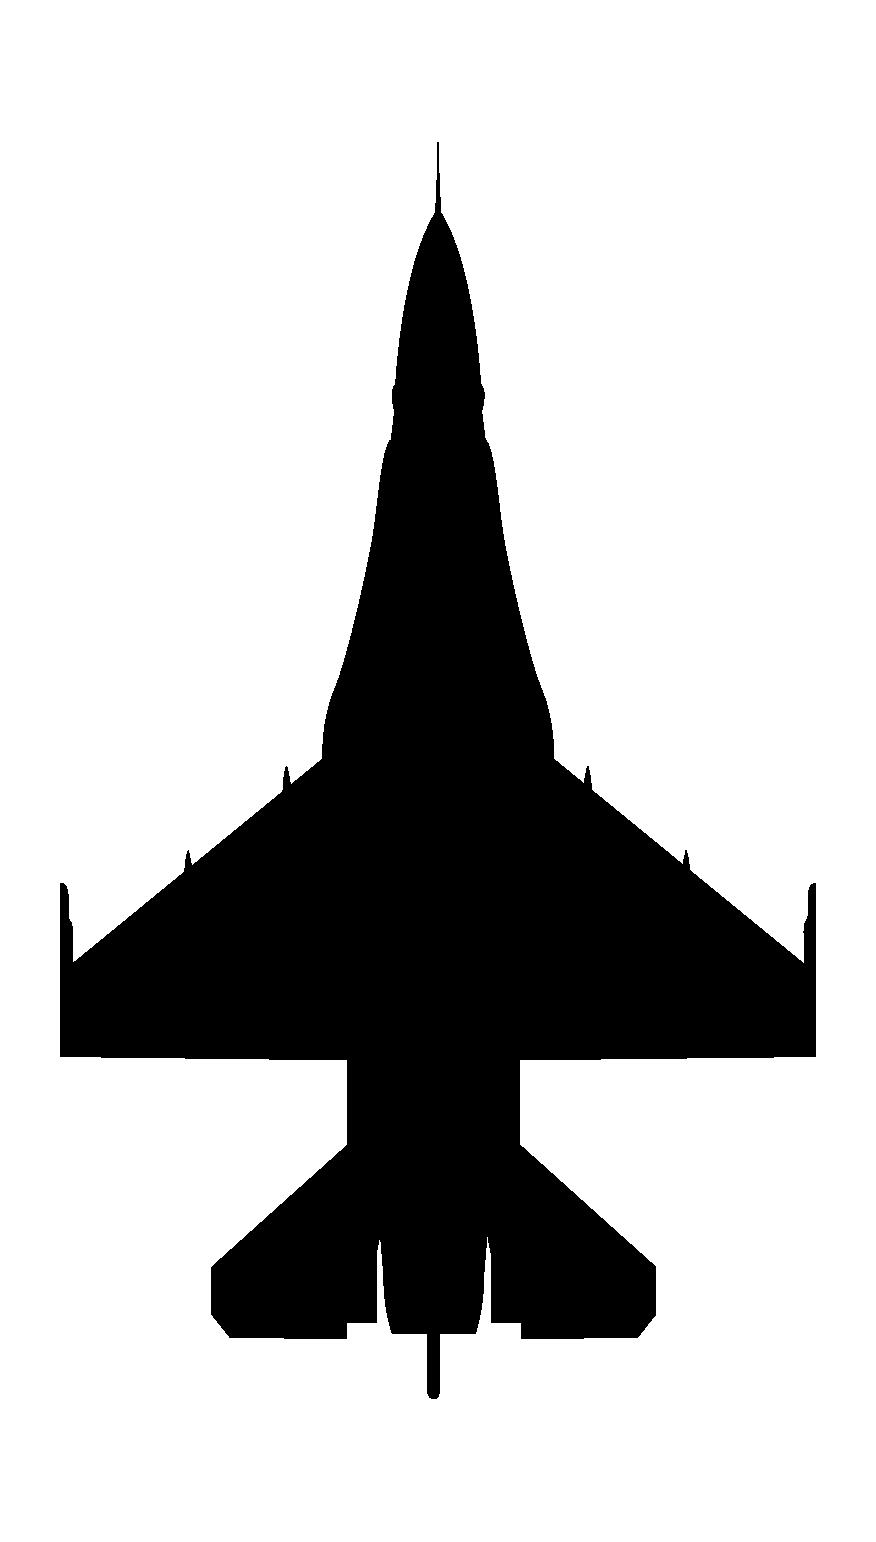
\includegraphics[
                width=7.5mm,
            ]{diagrams/aircraft/silhouette_f16_top.pdf}
        };
        
        \node[yshift=-2mm] (2fig) at (2) {
            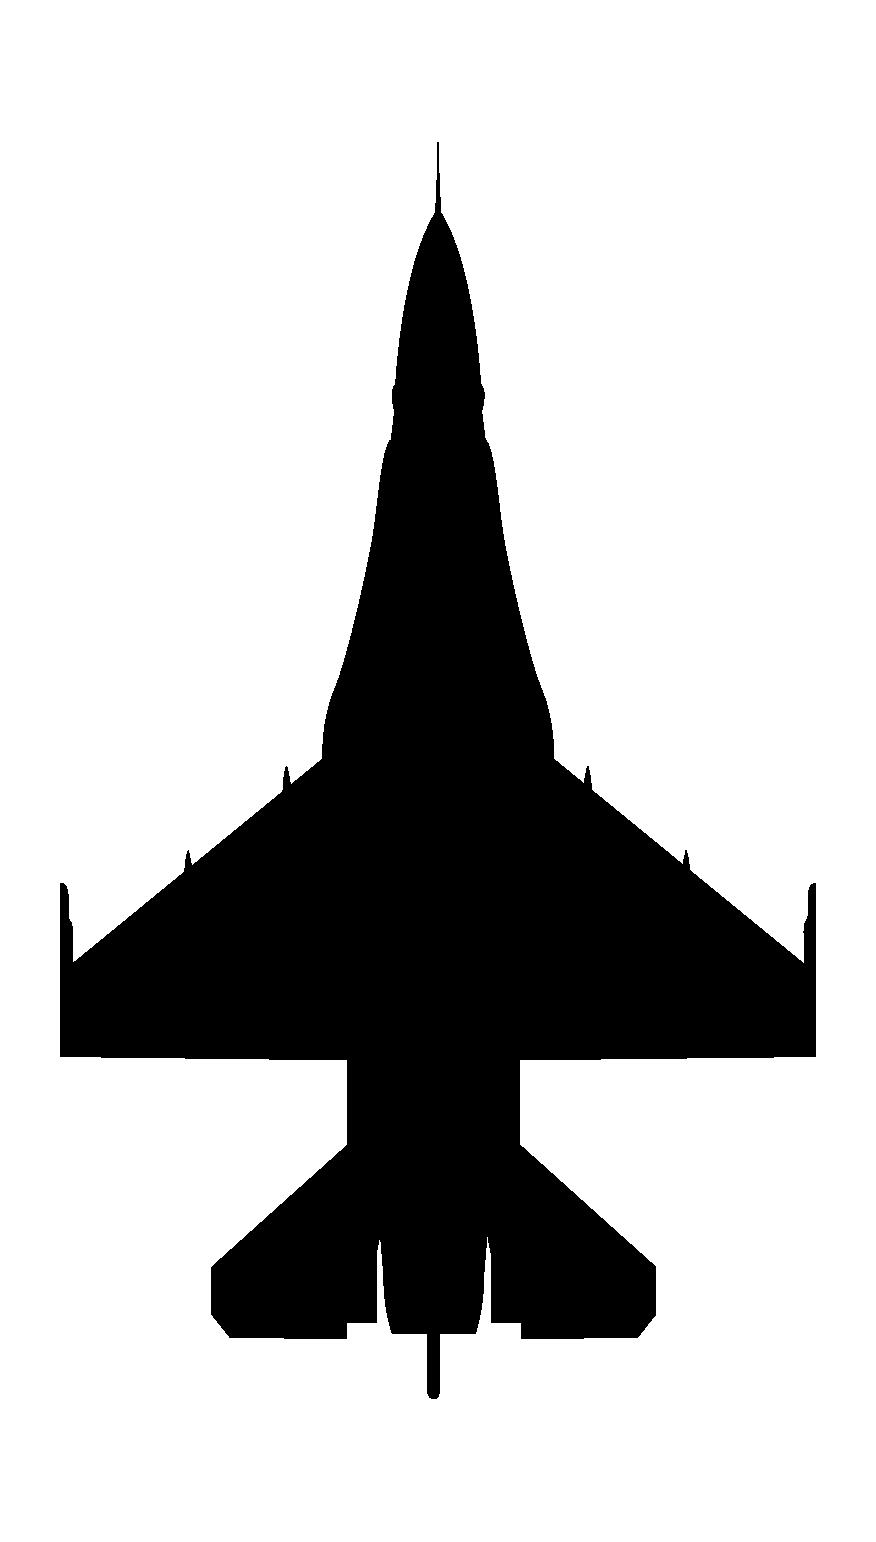
\includegraphics[
                width=7.5mm,
            ]{diagrams/aircraft/silhouette_f16_top.pdf}
        };

        \node[yshift=-2mm] (3fig) at (3) {
            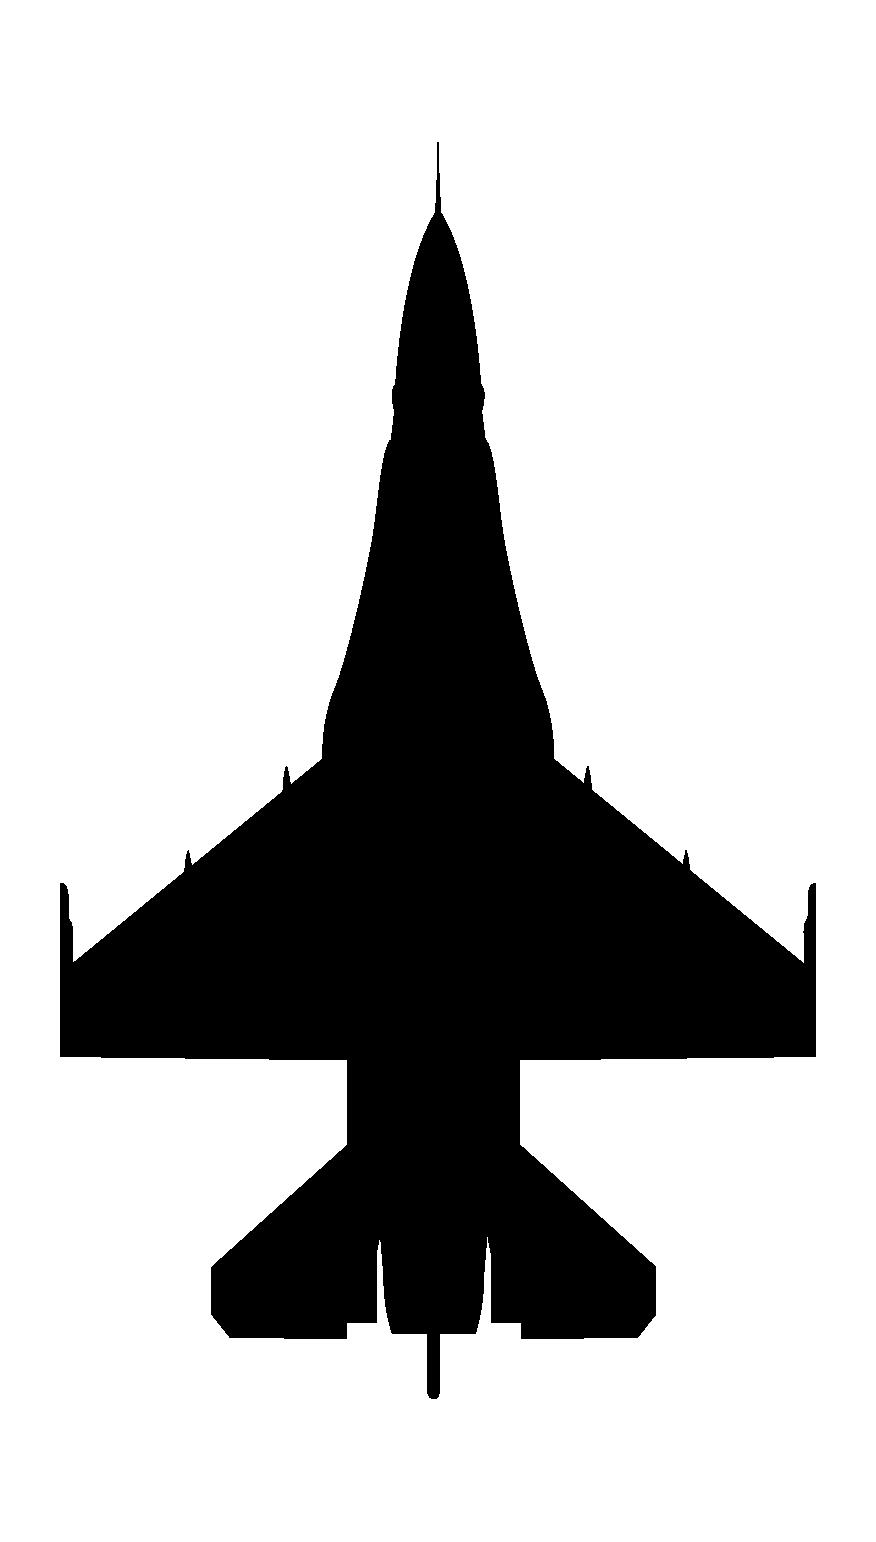
\includegraphics[
                width=7.5mm,
            ]{diagrams/aircraft/silhouette_f16_top.pdf}
        };
        
        \node[yshift=-2mm] (4fig) at (4) {
            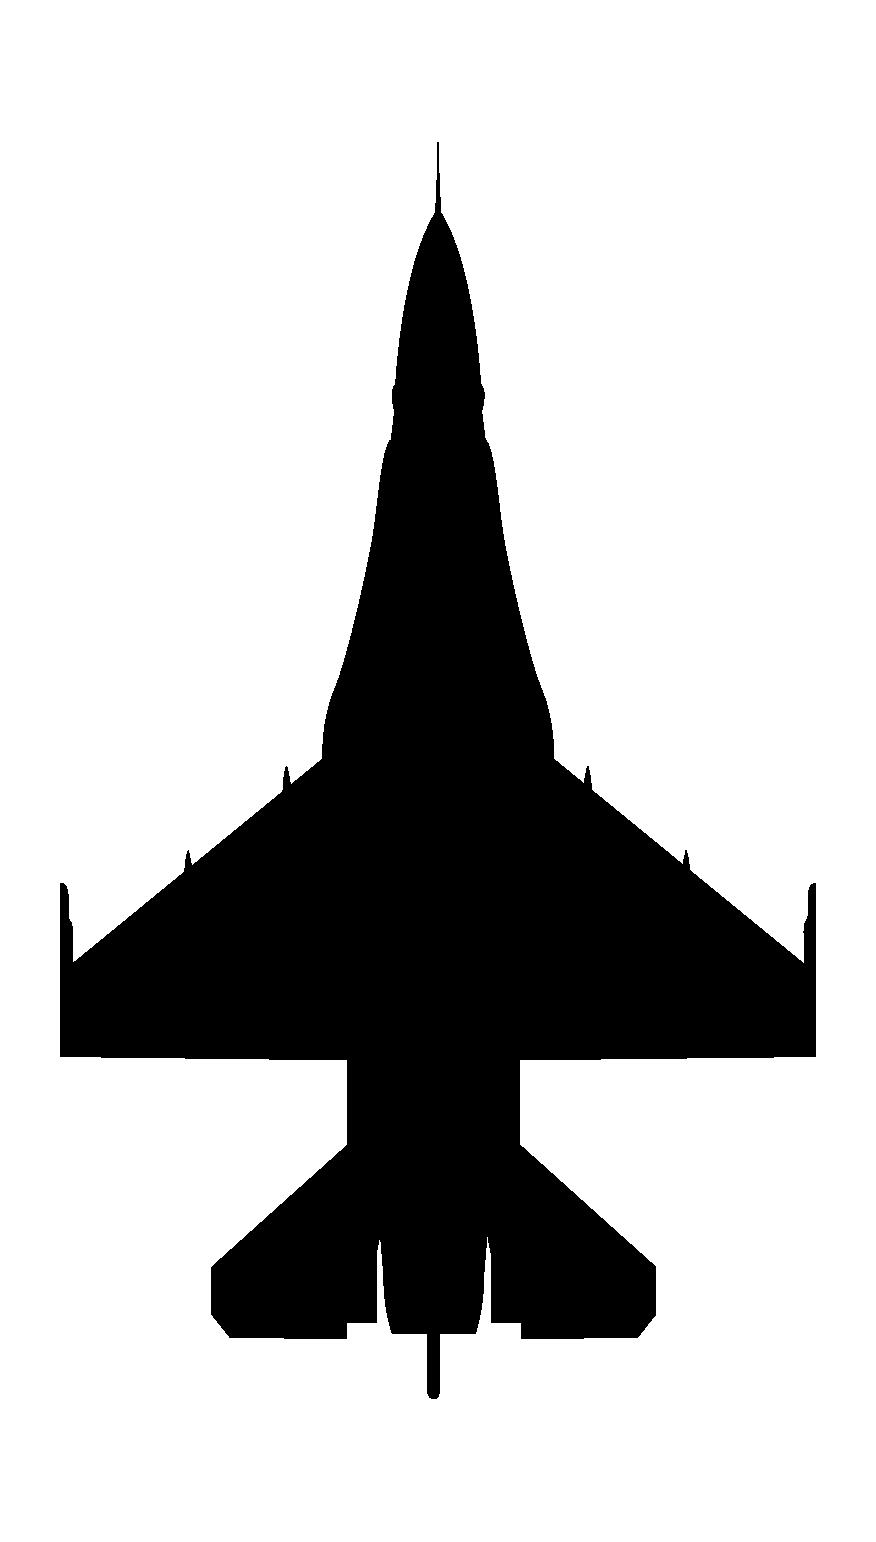
\includegraphics[
                width=7.5mm,
            ]{diagrams/aircraft/silhouette_f16_top.pdf}
        };

        \node[anchor=north, font=\footnotesize] (1label) at (1fig.south) {1};
        \node[anchor=north, font=\footnotesize] (2label) at (2fig.south) {2};
        \node[anchor=north, font=\footnotesize] (3label) at (3fig.south) {3};
        \node[anchor=north, font=\footnotesize] (4label) at (4fig.south) {4};

    \end{tikzpicture}
    \caption{Fluid-four formation}
    \label{fig:supp_fig:form:fluidfour}
\end{figure}

\begin{figure}[htbp]
    \centering
    \begin{minipage}[b]{0.5\textwidth}
        \centering
        \begin{tikzpicture}[figstyle]
            
            \coordinate (1) at (0,0);
            \coordinate (2) at ($(1)+(-150:15)$);
            \coordinate (3) at ($(1)+(-30:15)$);
            \coordinate (4) at ($(3)+(-30:15)$);

            \node[yshift=-2mm] (1fig) at (1) {
                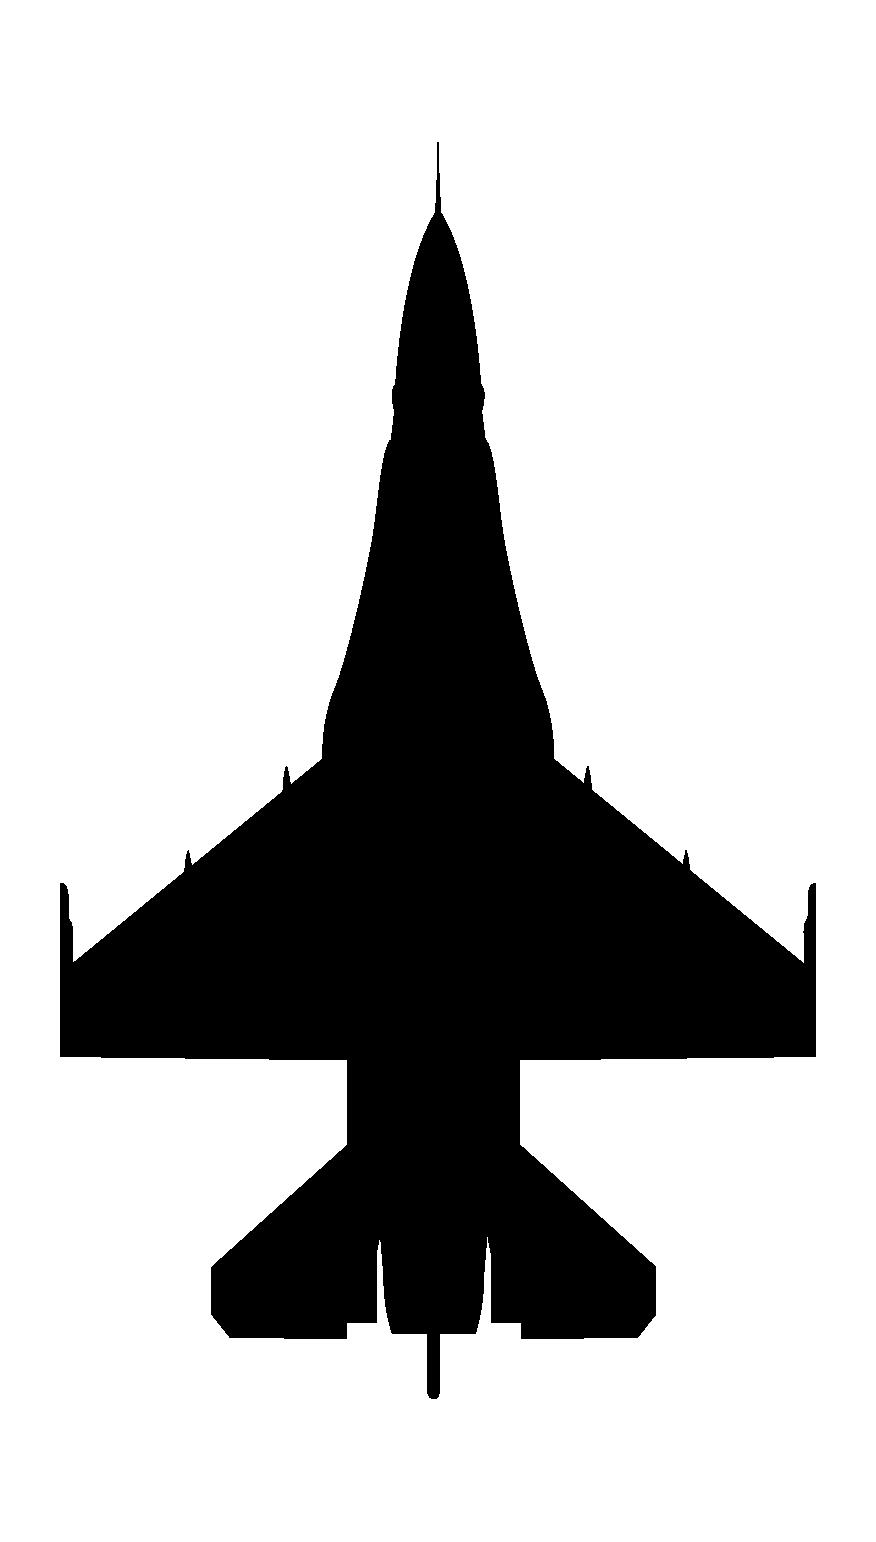
\includegraphics[
                    width=7.5mm,
                ]{diagrams/aircraft/silhouette_f16_top.pdf}
            };
            
            \node[yshift=-2mm] (2fig) at (2) {
                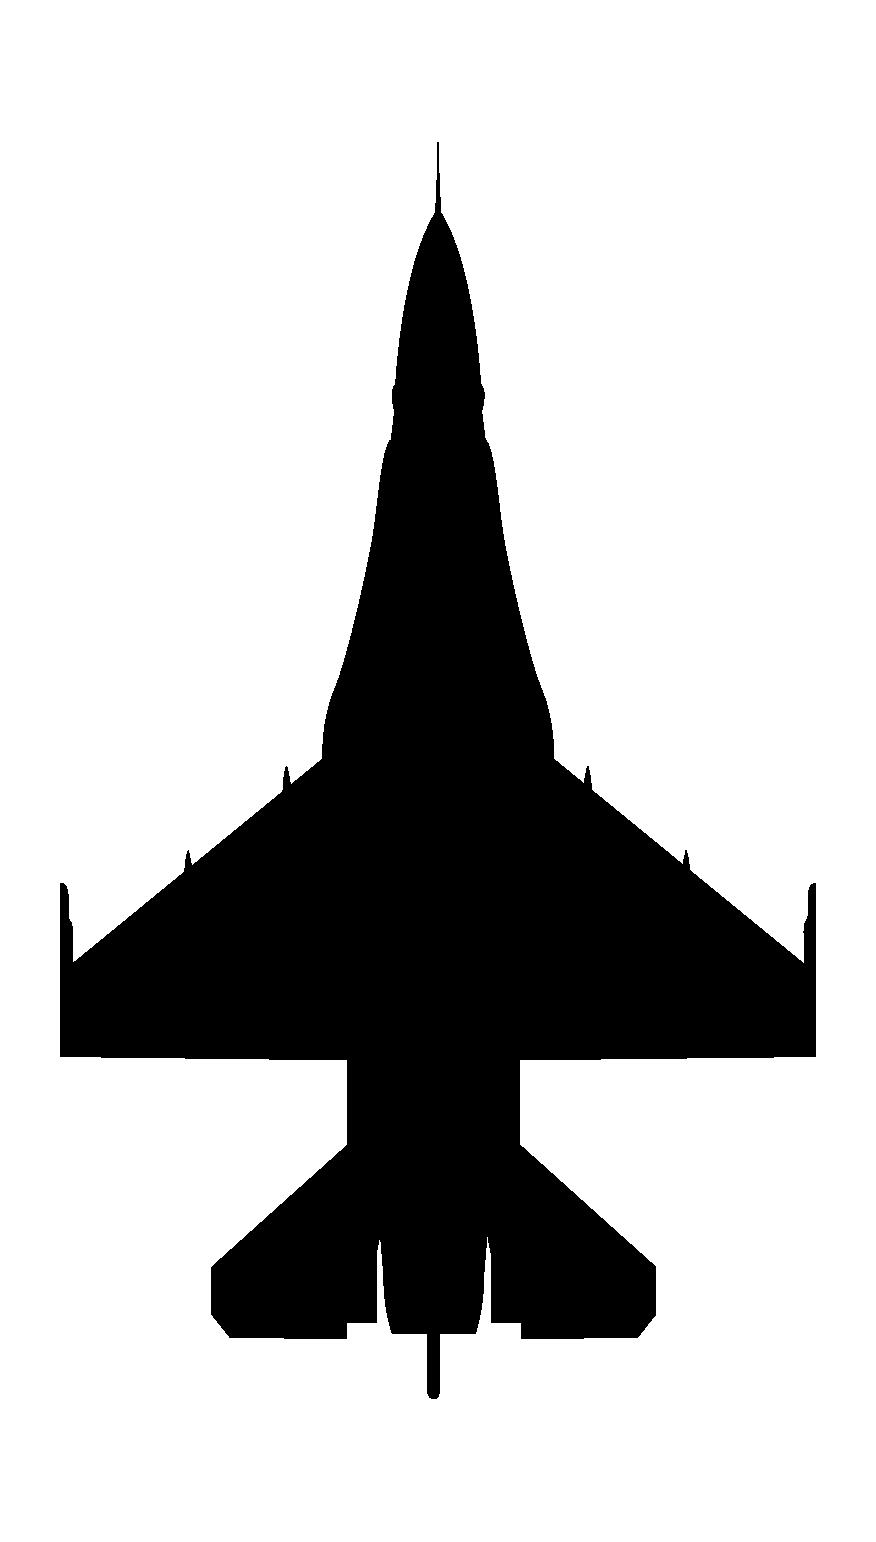
\includegraphics[
                    width=7.5mm,
                ]{diagrams/aircraft/silhouette_f16_top.pdf}
            };

            \node[yshift=-2mm] (3fig) at (3) {
                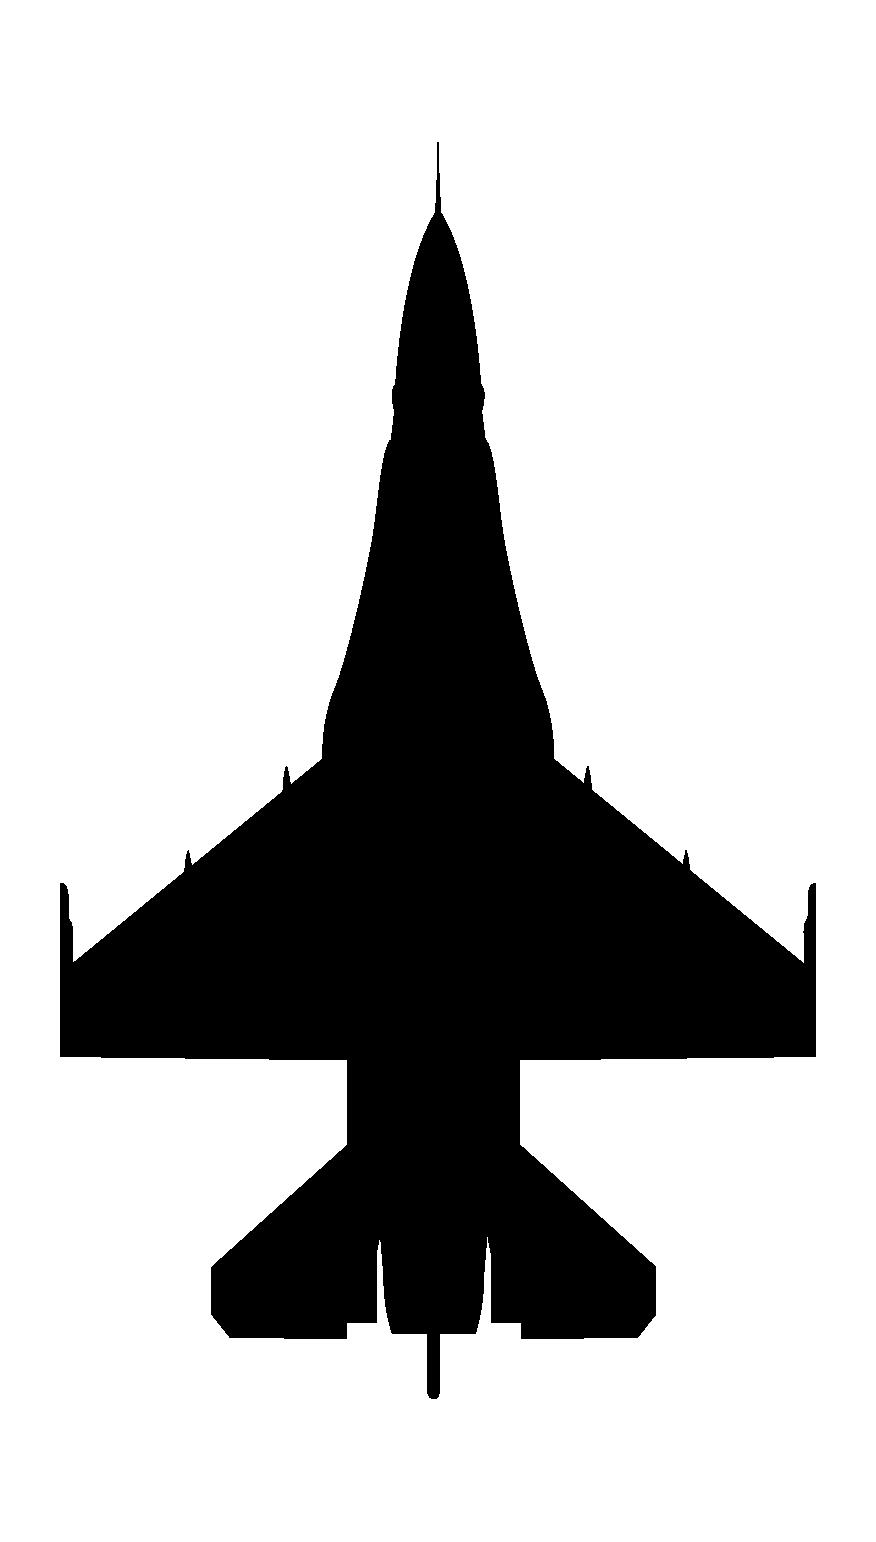
\includegraphics[
                    width=7.5mm,
                ]{diagrams/aircraft/silhouette_f16_top.pdf}
            };
            
            \node[yshift=-2mm] (4fig) at (4) {
                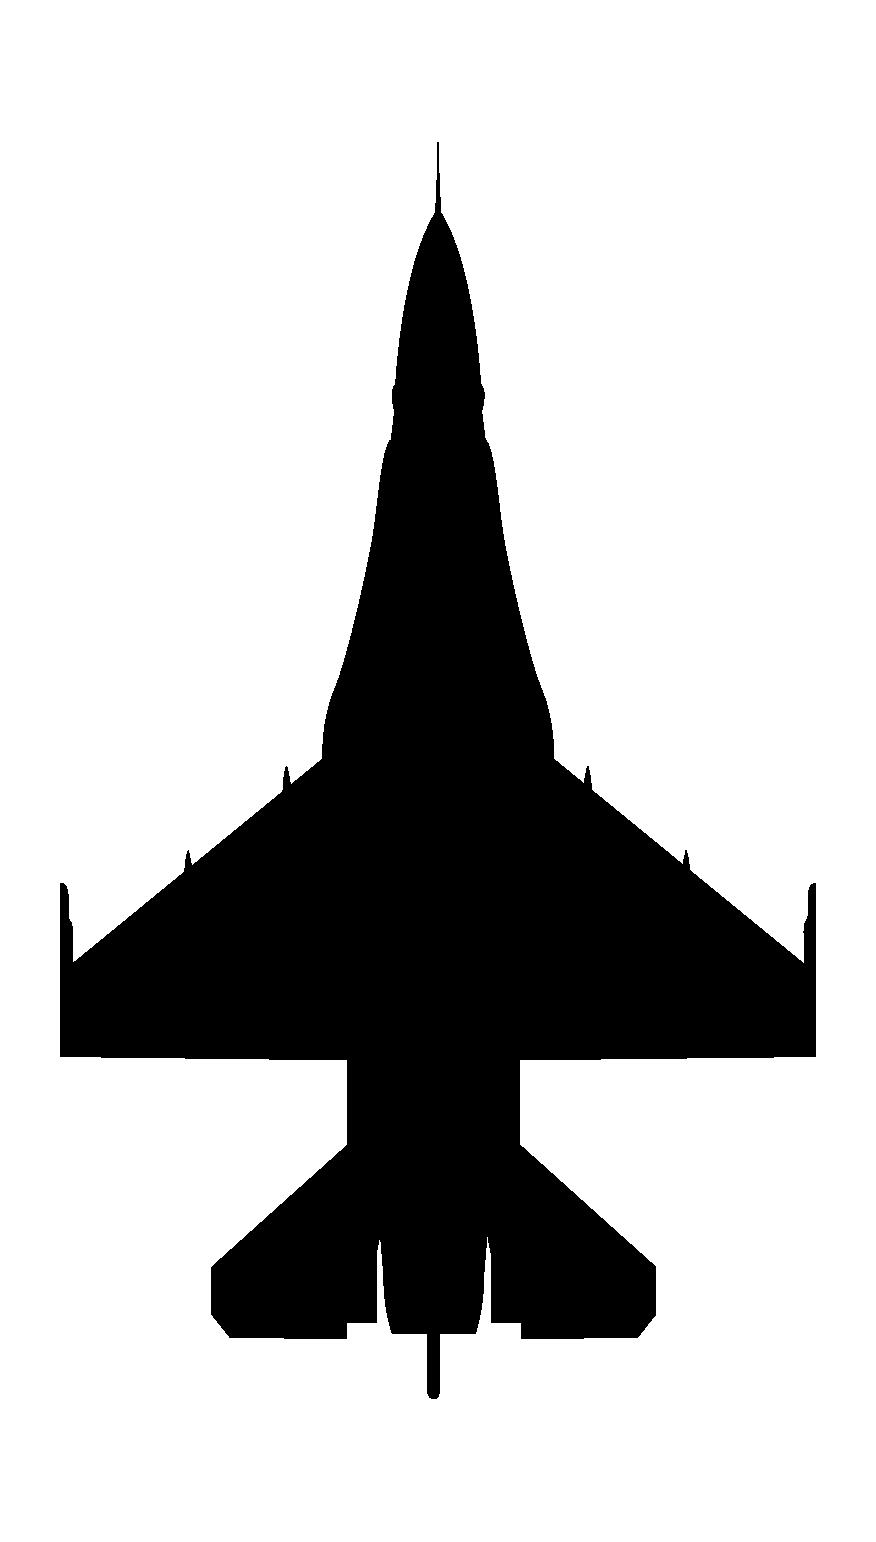
\includegraphics[
                    width=7.5mm,
                ]{diagrams/aircraft/silhouette_f16_top.pdf}
            };

            \node[anchor=north, font=\footnotesize] (1label) at (1fig.south) {1};
            \node[anchor=north, font=\footnotesize] (2label) at (2fig.south) {2};
            \node[anchor=north, font=\footnotesize] (3label) at (3fig.south) {3};
            \node[anchor=north, font=\footnotesize] (4label) at (4fig.south) {4};

        \end{tikzpicture}
        \caption{Fingertip formation}
        \label{fig:supp_fig:form:fingertip}
    \end{minipage}%
    \begin{minipage}[b]{0.5\textwidth}
        \centering
        \begin{tikzpicture}[figstyle]
            
            \coordinate (1) at (0,0);
            \coordinate (2) at ($(1)+(-150:20)$);
            \coordinate (3) at ($(1)+(-30:20)$);
            \coordinate (4) at ($(3)+(-150:20)$);

            \node[yshift=-2mm] (1fig) at (1) {
                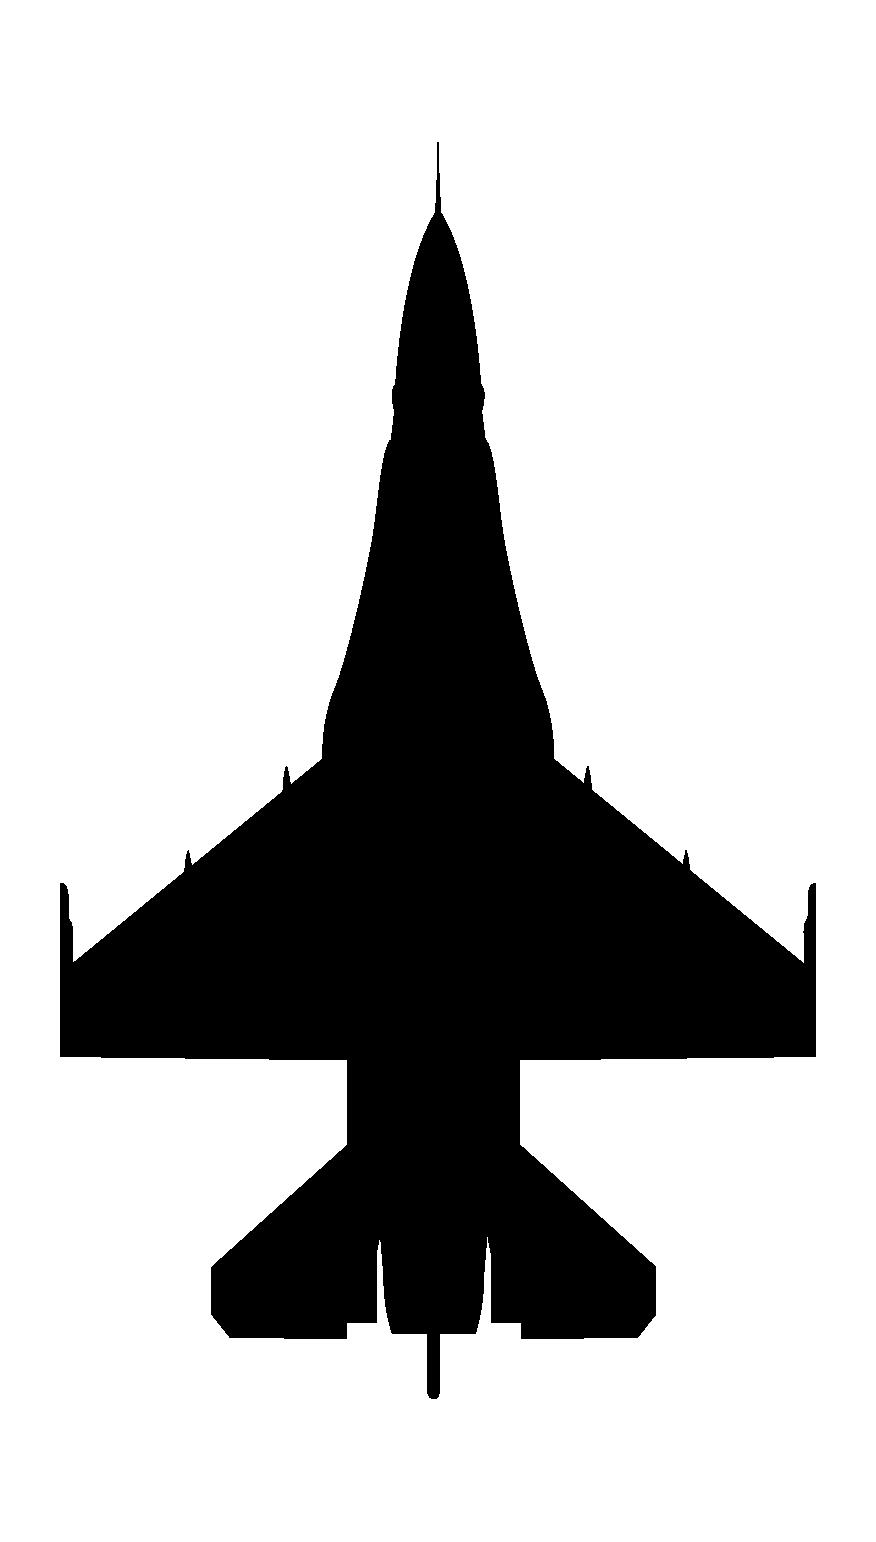
\includegraphics[
                    width=7.5mm,
                ]{diagrams/aircraft/silhouette_f16_top.pdf}
            };
            
            \node[yshift=-2mm] (2fig) at (2) {
                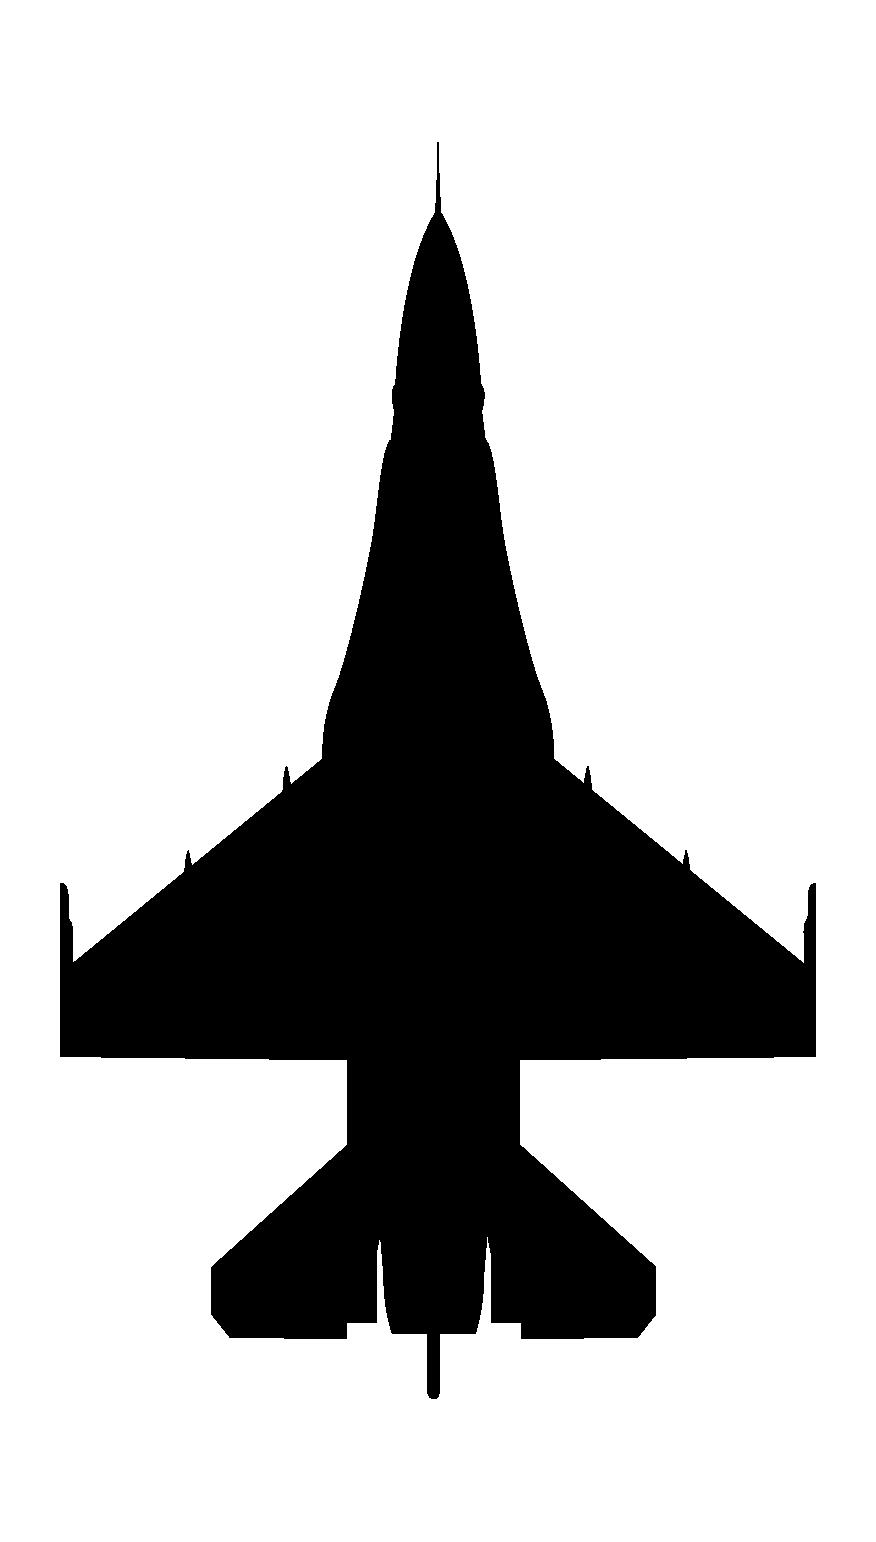
\includegraphics[
                    width=7.5mm,
                ]{diagrams/aircraft/silhouette_f16_top.pdf}
            };

            \node[yshift=-2mm] (3fig) at (3) {
                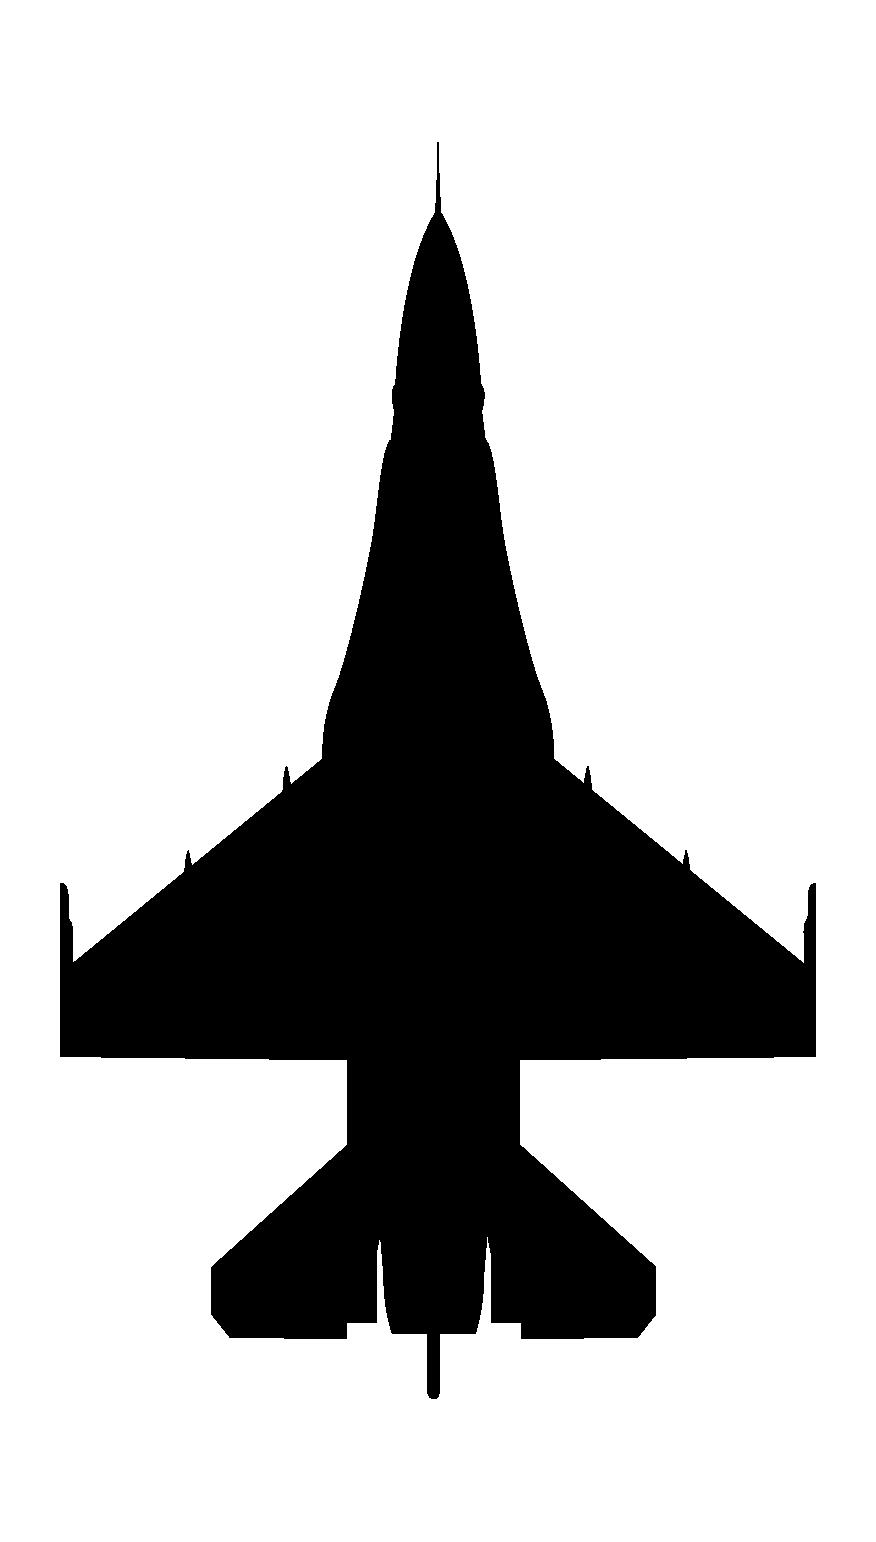
\includegraphics[
                    width=7.5mm,
                ]{diagrams/aircraft/silhouette_f16_top.pdf}
            };
            
            \node[yshift=-2mm] (4fig) at (4) {
                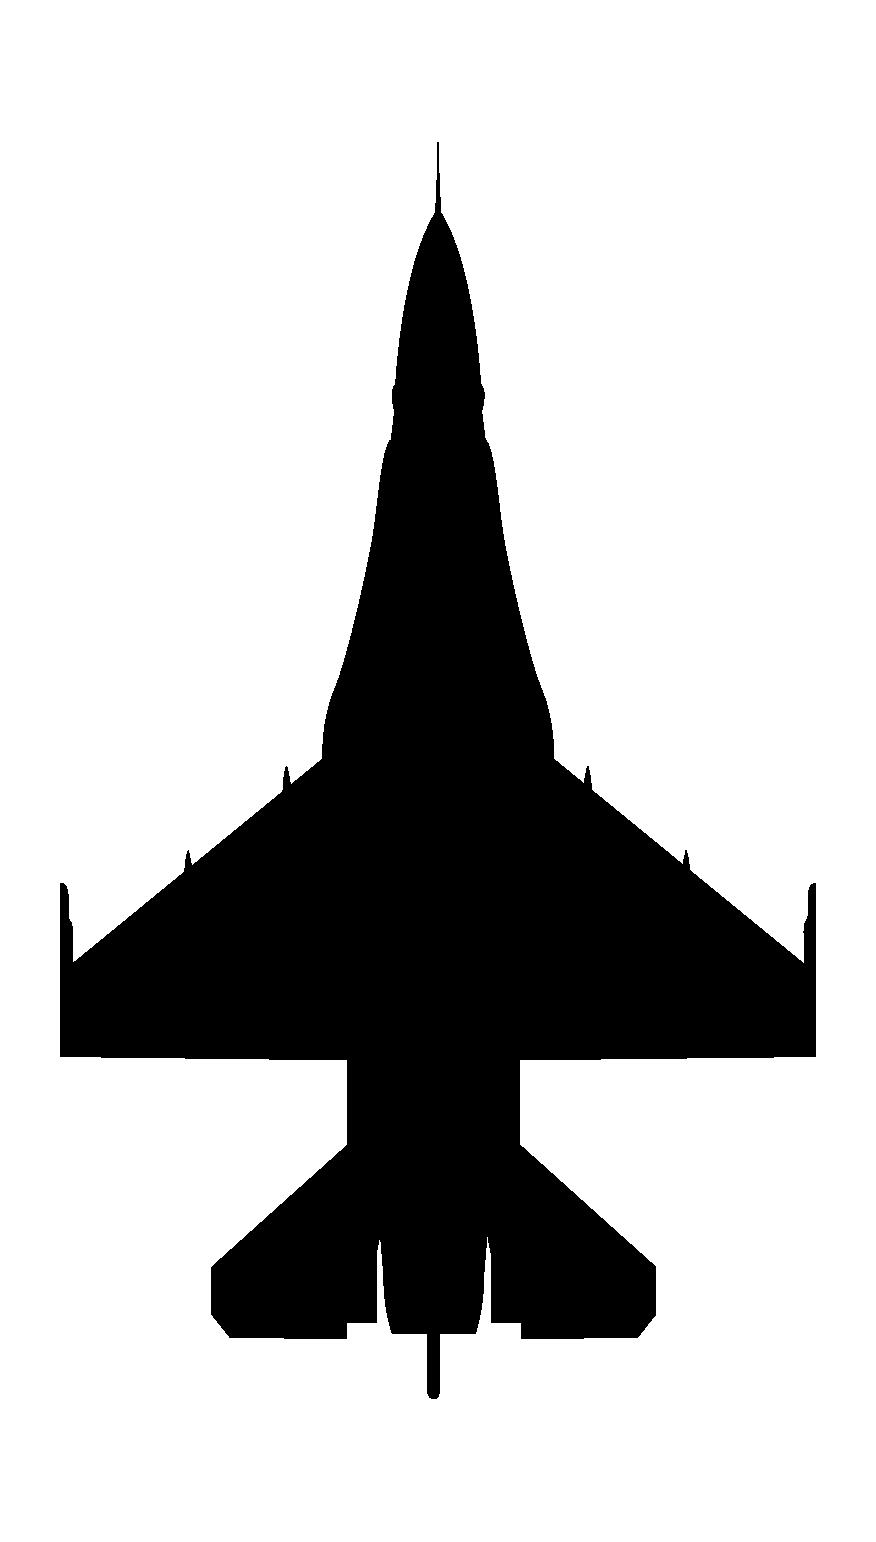
\includegraphics[
                    width=7.5mm,
                ]{diagrams/aircraft/silhouette_f16_top.pdf}
            };

            \node[anchor=north, font=\footnotesize] (1label) at (1fig.south) {1};
            \node[anchor=north, font=\footnotesize] (2label) at (2fig.south) {2};
            \node[anchor=north, font=\footnotesize] (3label) at (3fig.south) {3};
            \node[anchor=north, font=\footnotesize] (4label) at (4fig.south) {4};

        \end{tikzpicture}
        \caption{Diamond formation}
        \label{fig:supp_fig:form:diamond}
    \end{minipage}
\end{figure}

\begin{figure}[htbp]
    \centering
    \begin{minipage}[b]{0.5\textwidth}
        \centering
        \begin{tikzpicture}[figstyle]
            
            \coordinate (1) at (0,0);
            \coordinate (2) at ($(1)+(-90:15)$);
            \coordinate (3) at ($(2)+(-90:15)$);
            \coordinate (4) at ($(3)+(-90:15)$);

            \node[yshift=-2mm] (1fig) at (1) {
                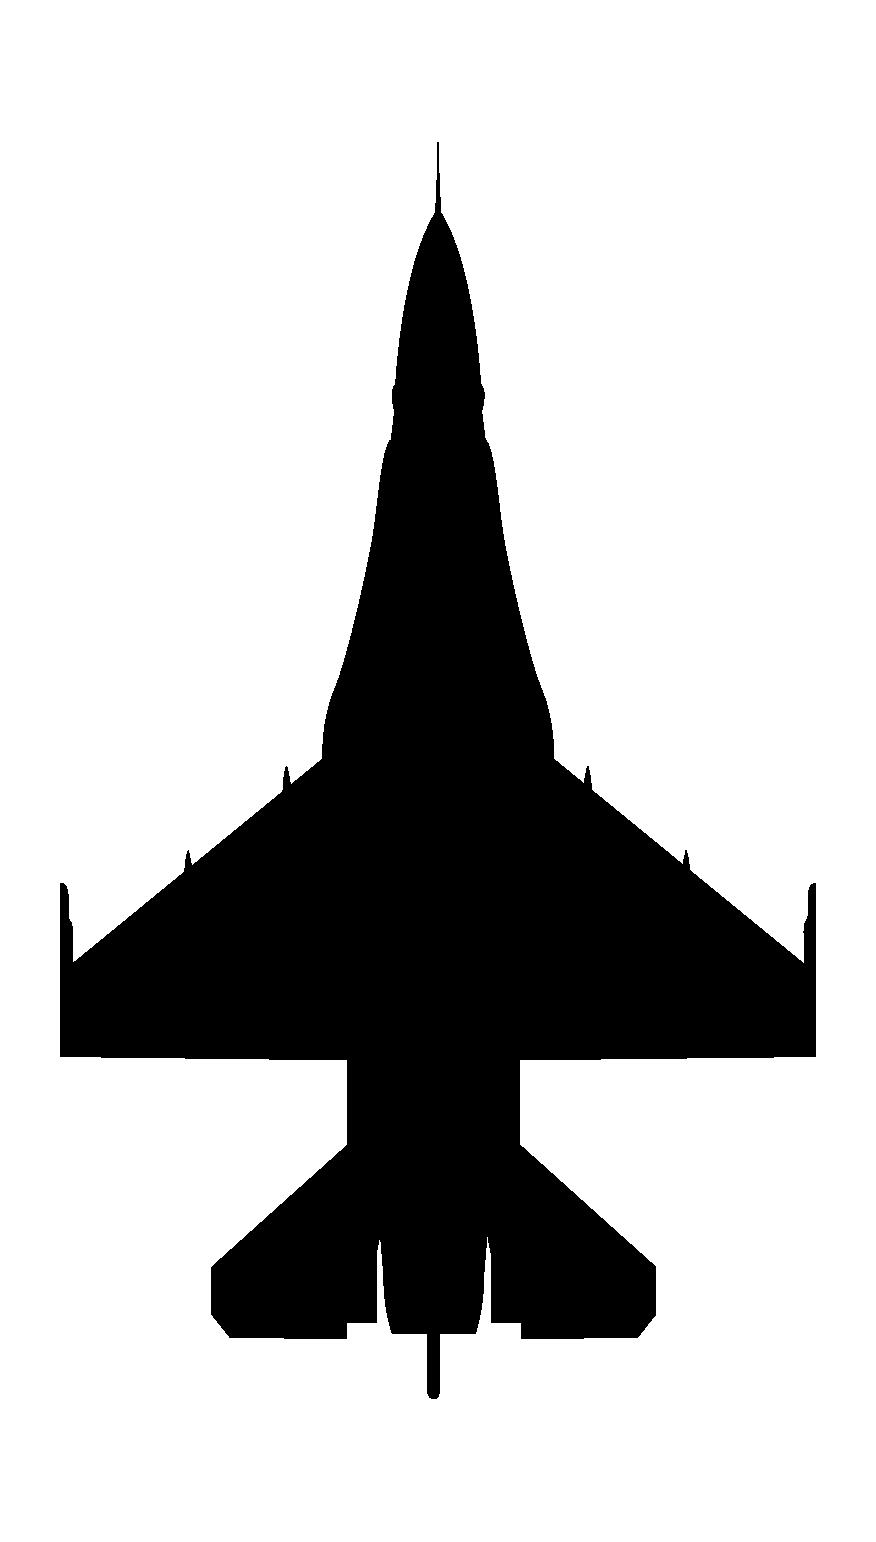
\includegraphics[
                    width=7.5mm,
                ]{diagrams/aircraft/silhouette_f16_top.pdf}
            };
            
            \node[yshift=-2mm] (2fig) at (2) {
                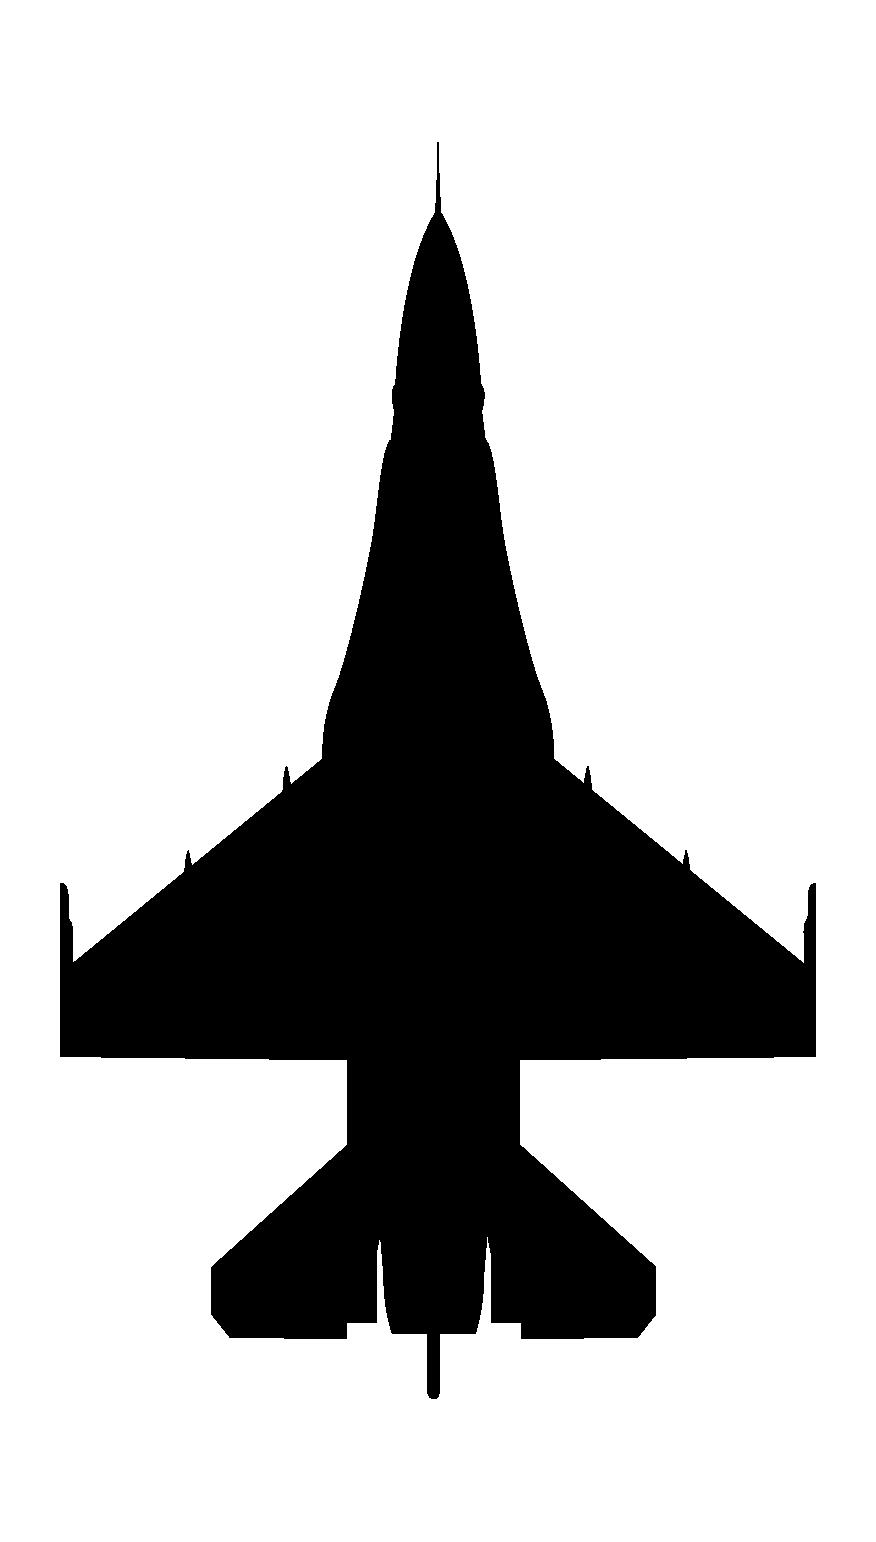
\includegraphics[
                    width=7.5mm,
                ]{diagrams/aircraft/silhouette_f16_top.pdf}
            };

            \node[yshift=-2mm] (3fig) at (3) {
                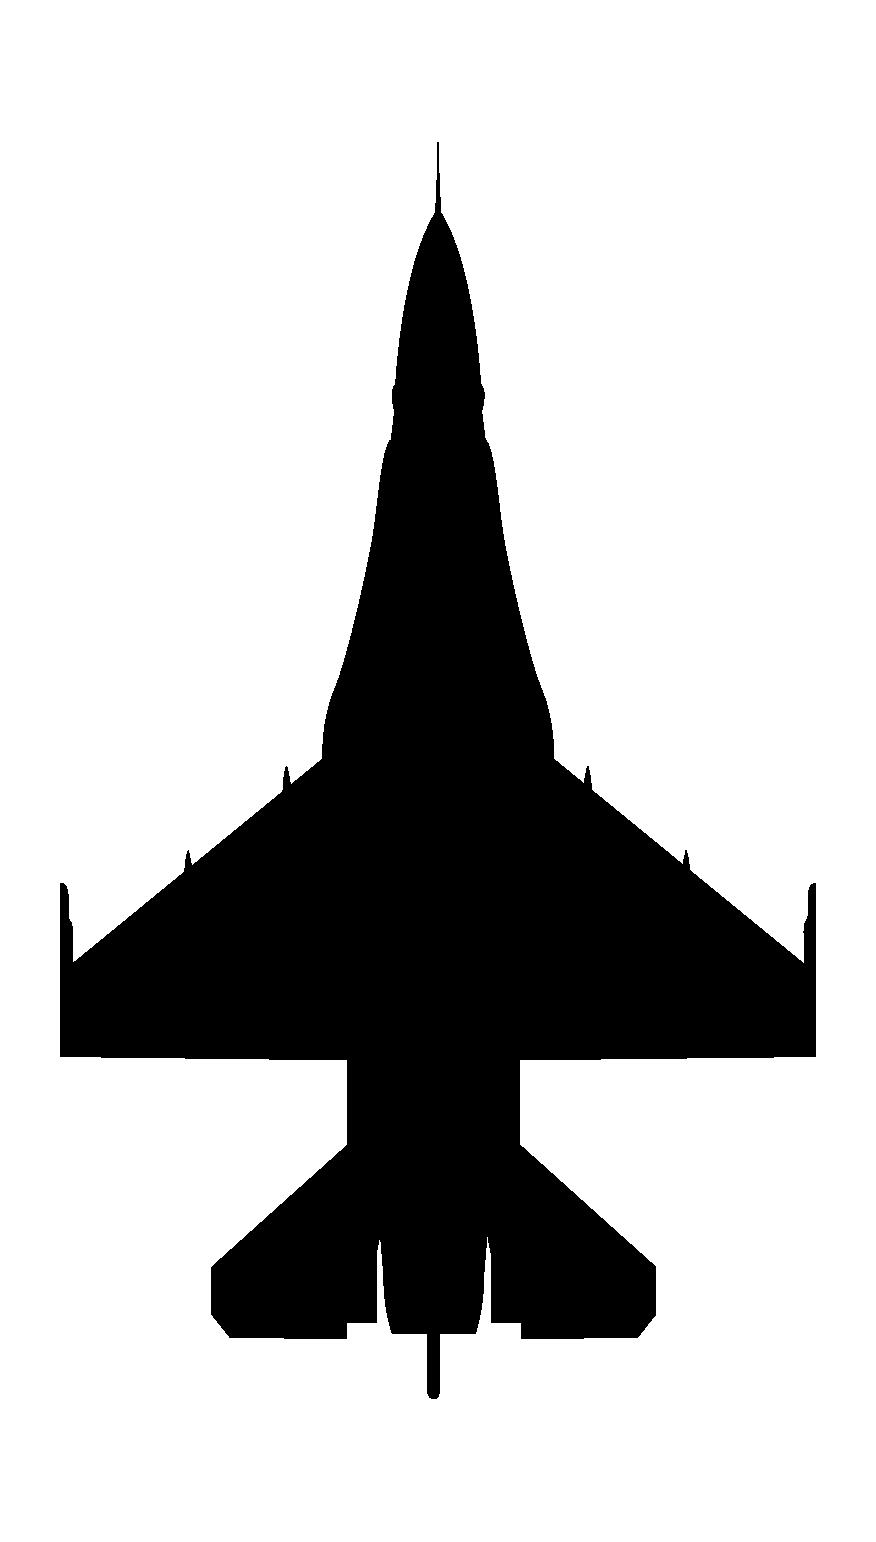
\includegraphics[
                    width=7.5mm,
                ]{diagrams/aircraft/silhouette_f16_top.pdf}
            };
            
            \node[yshift=-2mm] (4fig) at (4) {
                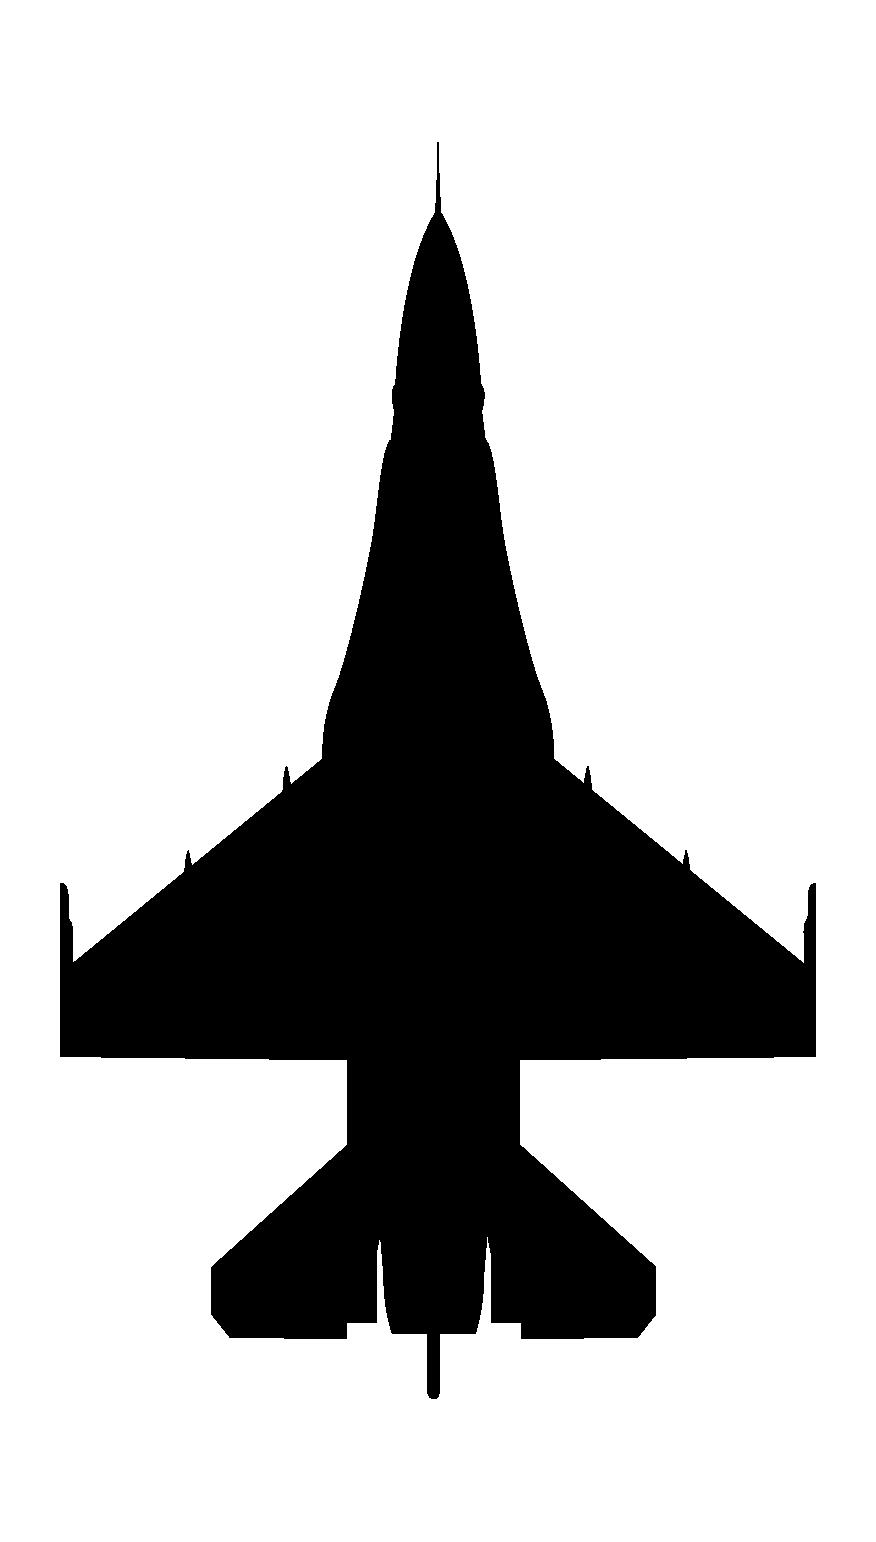
\includegraphics[
                    width=7.5mm,
                ]{diagrams/aircraft/silhouette_f16_top.pdf}
            };

            \node[anchor=west, font=\footnotesize] (1label) at (1fig.east) {1};
            \node[anchor=west, font=\footnotesize] (2label) at (2fig.east) {2};
            \node[anchor=west, font=\footnotesize] (3label) at (3fig.east) {3};
            \node[anchor=west, font=\footnotesize] (4label) at (4fig.east) {4};

        \end{tikzpicture}
        \caption{Trail formation}
        \label{fig:supp_fig:form:trail}
    \end{minipage}%
    \begin{minipage}[b]{0.5\textwidth}
        \centering
        \begin{tikzpicture}[figstyle]
            
            \coordinate (1) at (0,0);
            \coordinate (2) at ($(1)+(0:15)$);
            \coordinate (3) at ($(2)+(0:15)$);
            \coordinate (4) at ($(3)+(0:15)$);

            \node[yshift=-2mm] (1fig) at (1) {
                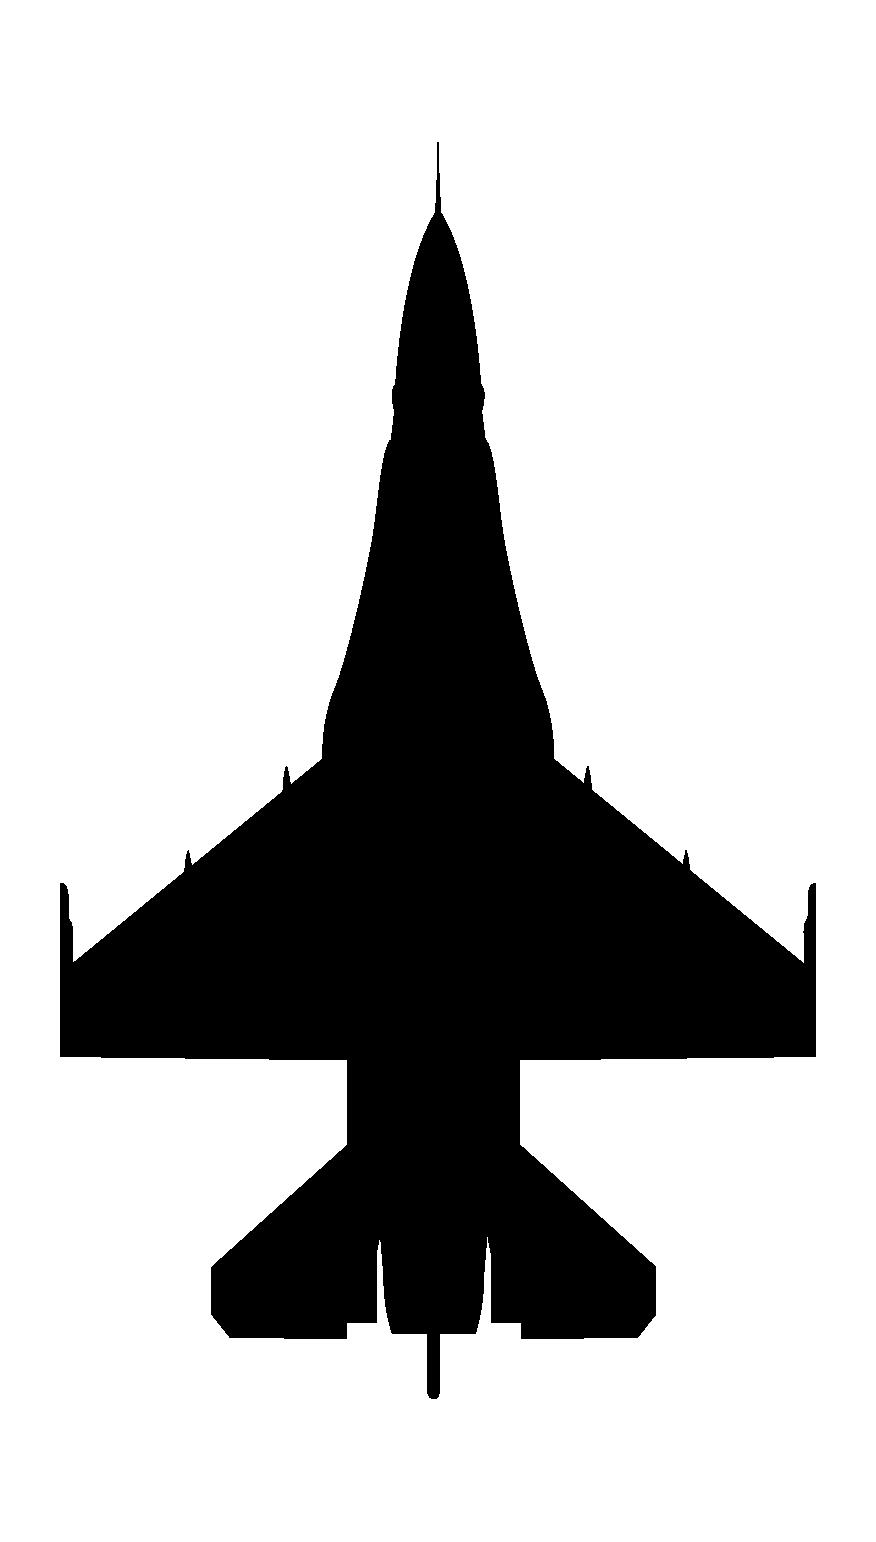
\includegraphics[
                    width=7.5mm,
                ]{diagrams/aircraft/silhouette_f16_top.pdf}
            };
            
            \node[yshift=-2mm] (2fig) at (2) {
                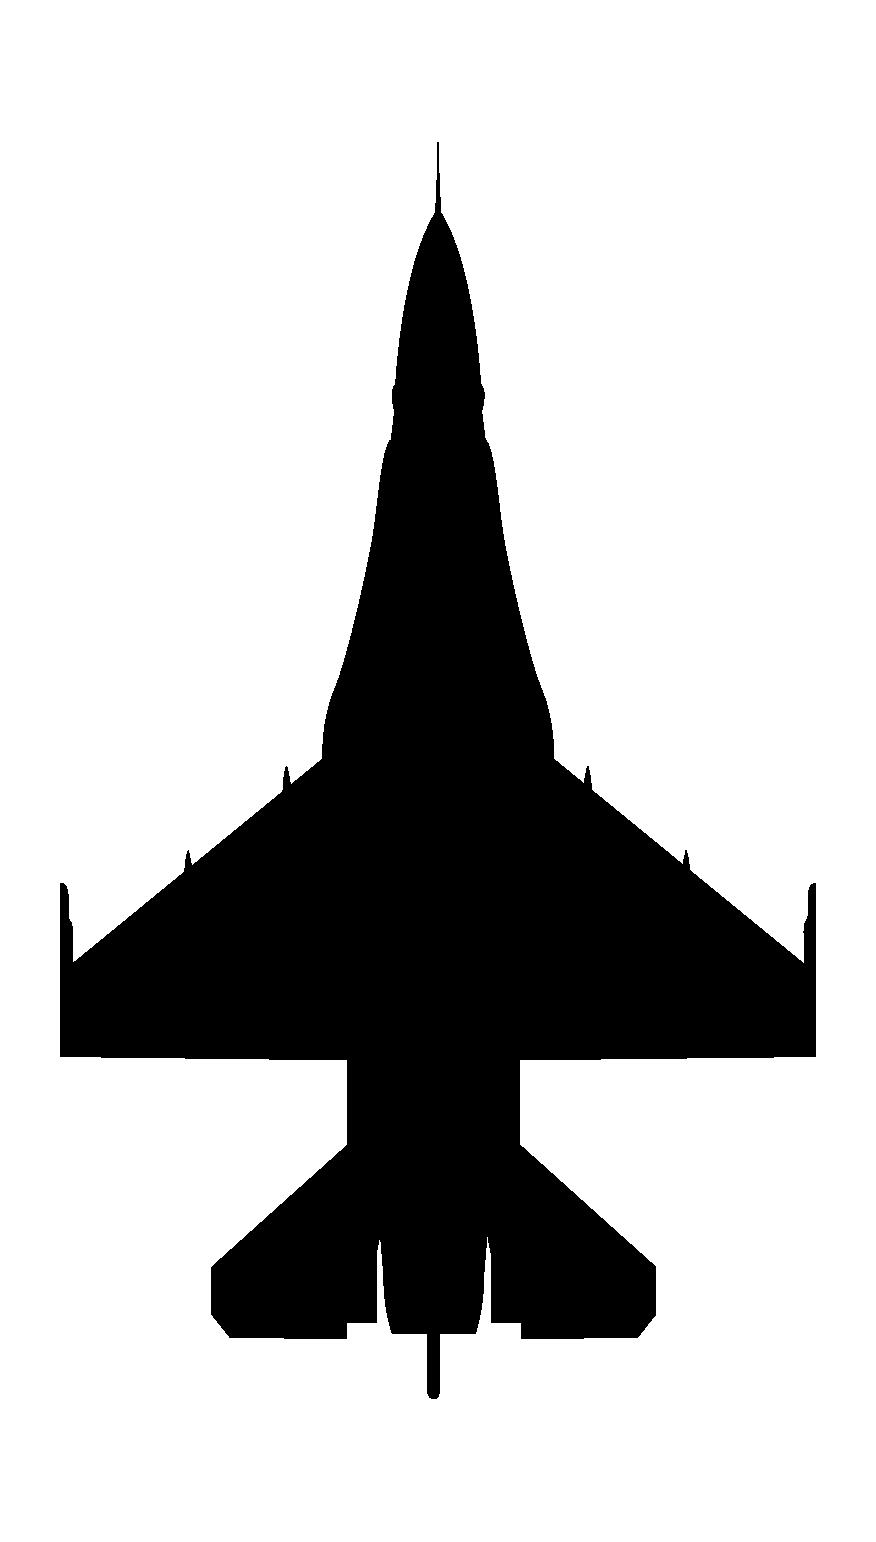
\includegraphics[
                    width=7.5mm,
                ]{diagrams/aircraft/silhouette_f16_top.pdf}
            };

            \node[yshift=-2mm] (3fig) at (3) {
                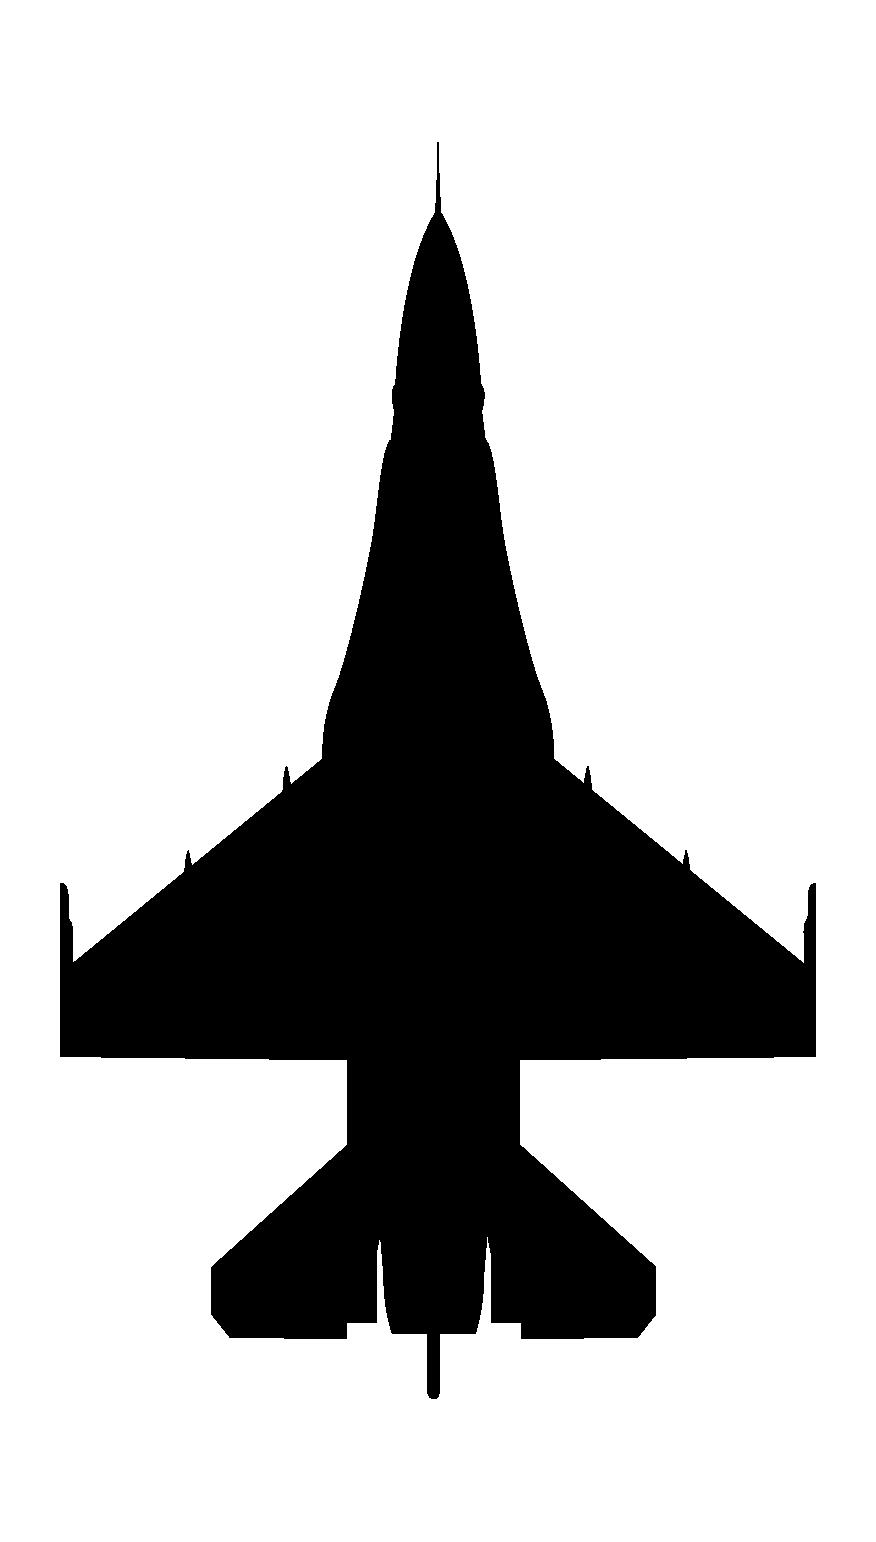
\includegraphics[
                    width=7.5mm,
                ]{diagrams/aircraft/silhouette_f16_top.pdf}
            };
            
            \node[yshift=-2mm] (4fig) at (4) {
                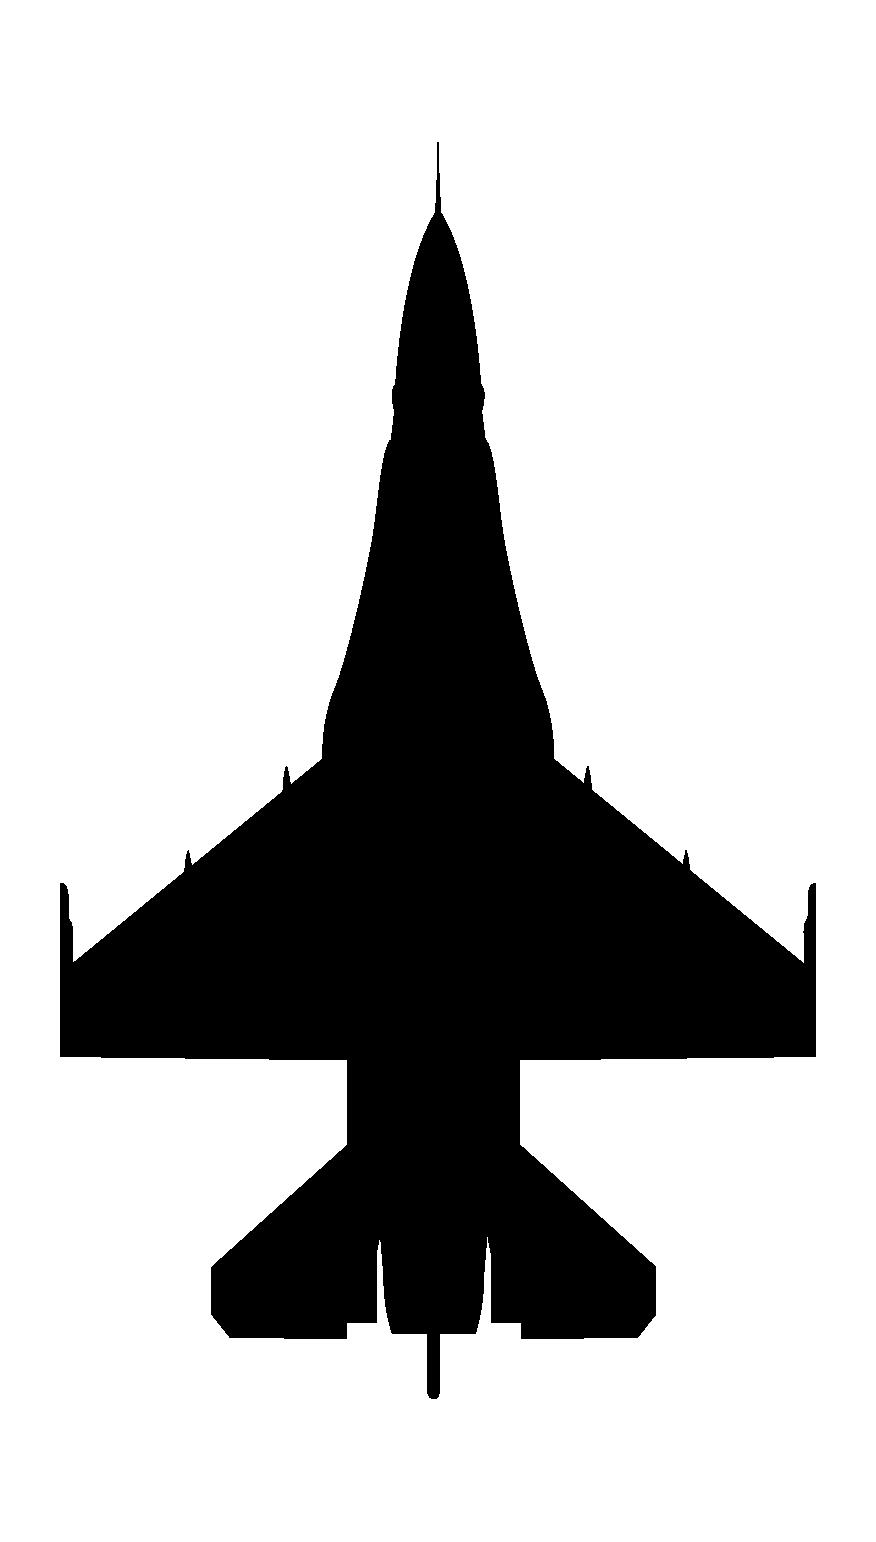
\includegraphics[
                    width=7.5mm,
                ]{diagrams/aircraft/silhouette_f16_top.pdf}
            };

            \node[anchor=north, font=\footnotesize] (1label) at (1fig.south) {1};
            \node[anchor=north, font=\footnotesize] (2label) at (2fig.south) {2};
            \node[anchor=north, font=\footnotesize] (3label) at (3fig.south) {3};
            \node[anchor=north, font=\footnotesize] (4label) at (4fig.south) {4};

        \end{tikzpicture}
        \caption{Spread formation}
        \label{fig:supp_fig:form:spread}
    \end{minipage}
\end{figure}

\clearpage

\subsection{TACTICAL TURNS}

\begin{tcoloritemize}
    \blueitem[Tactical Turn]
    \textbf{Maintains line abreast formation}
    
    \begin{itemize}
        \item flight member on outside must initiate turn
    \end{itemize}
    \medskip

    Reference \cref{fig:supp_fig:form:tacturn} for illustration
\end{tcoloritemize}

\begin{figure}[htbp]
    \centering
    \begin{subfigure}[b]{0.45\linewidth}
        \centering
        \begin{tikzpicture}[figstyle]
            
            \draw[->] 
            (0,0) -- 
            node[below, pos=0]{
                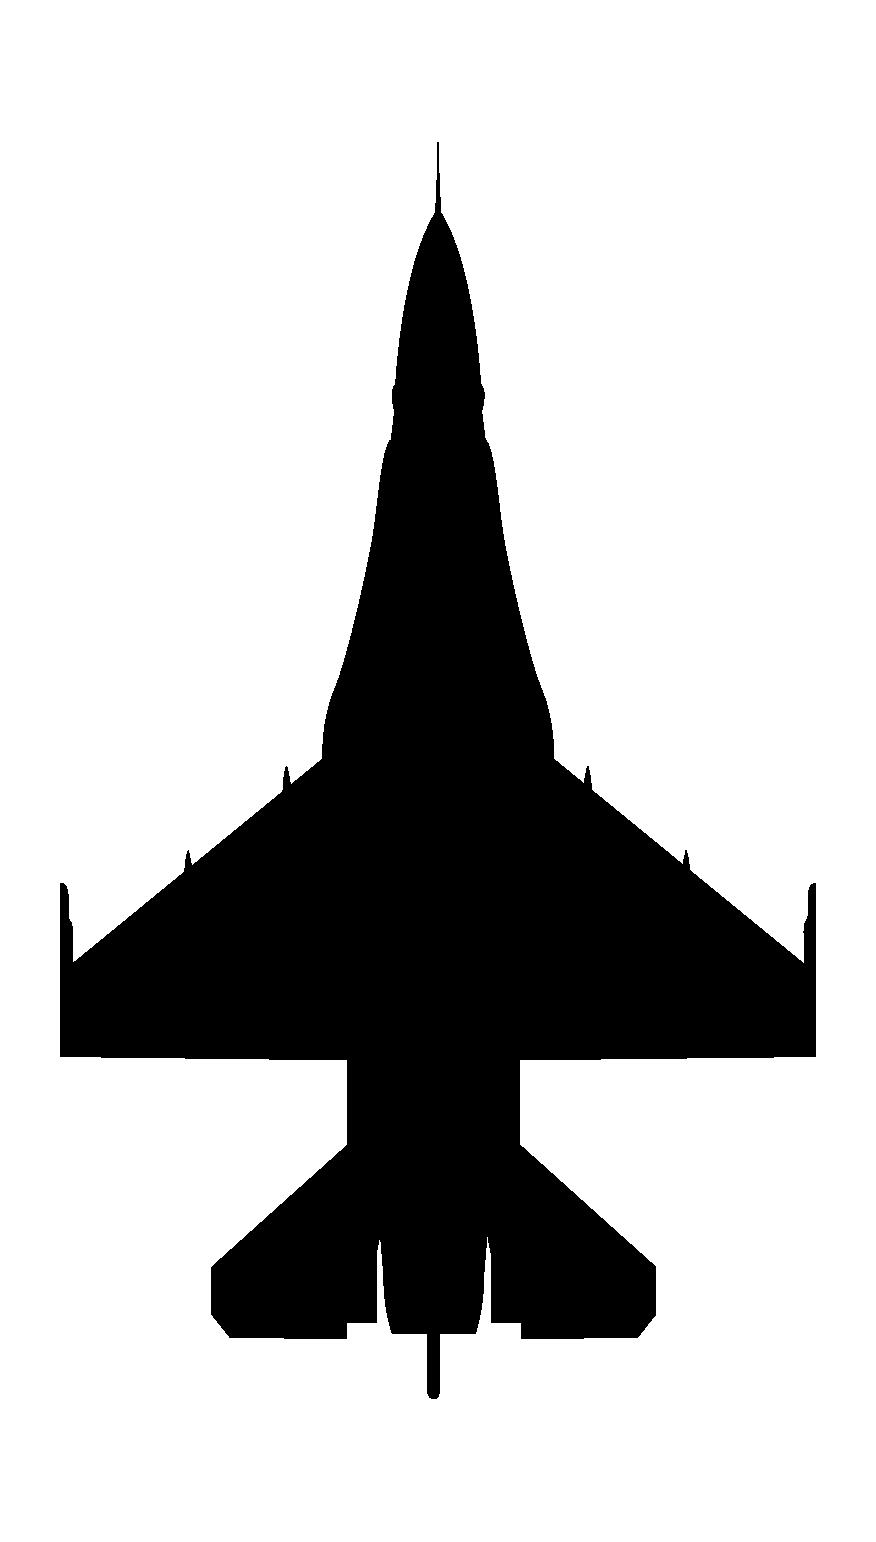
\includegraphics[
                width=7.5mm,
            ]{diagrams/aircraft/silhouette_f16_top.pdf}} 
            ++(0,10) 
            arc (180:90:10) 
            -- ++(20,0) 
            node[above, pos=1, rotate=-90]{
                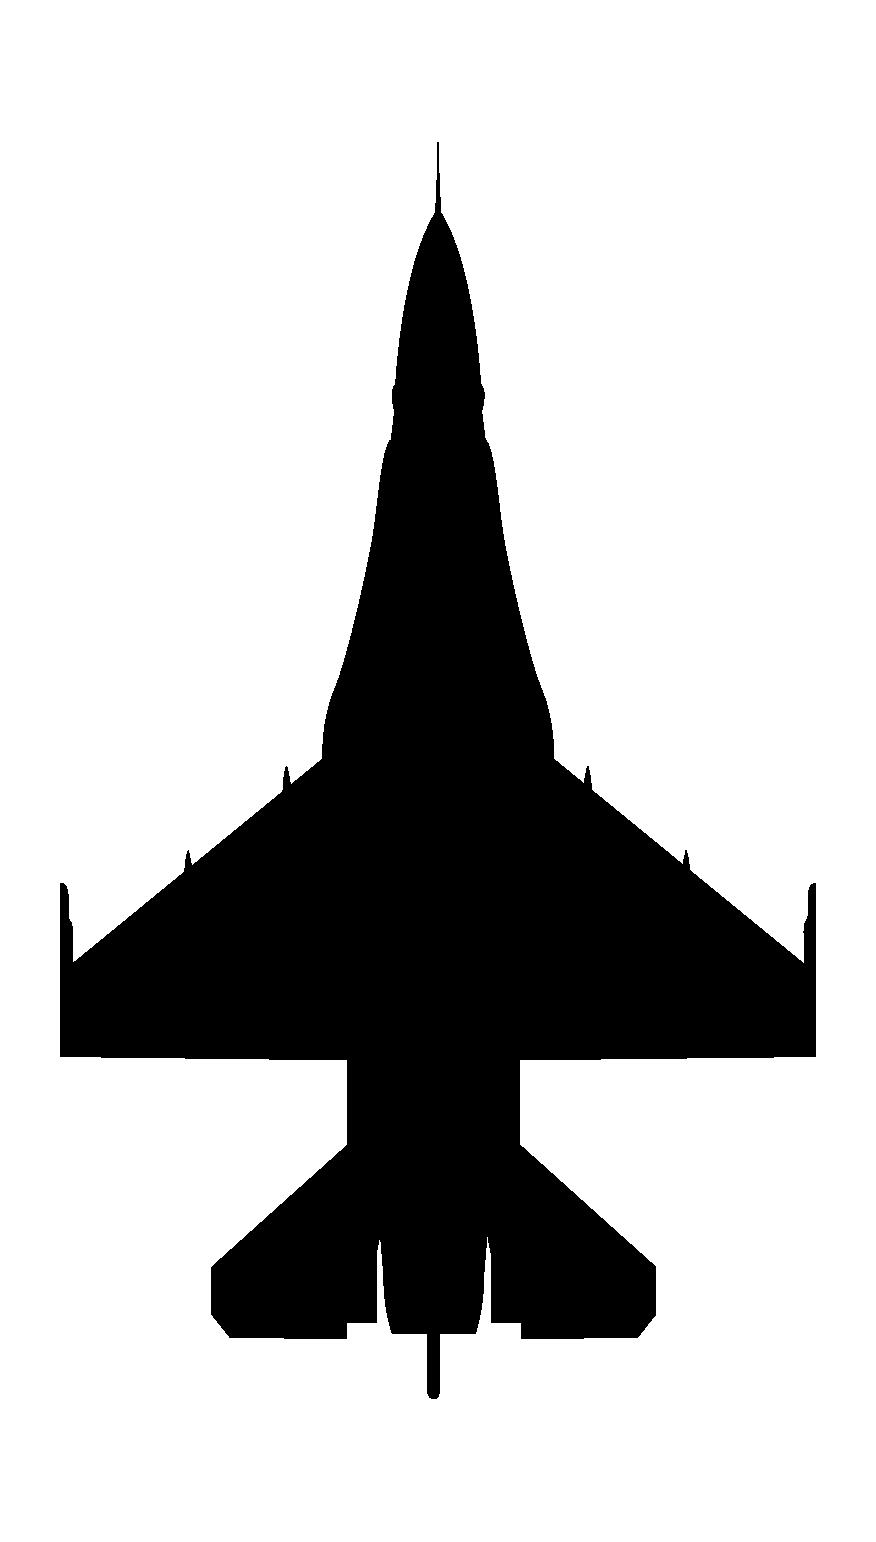
\includegraphics[
                    width=7.5mm,
            ]{diagrams/aircraft/silhouette_f16_top.pdf}};
                
            \draw[->] 
            (10,0) -- 
            node[below, pos=0]{
                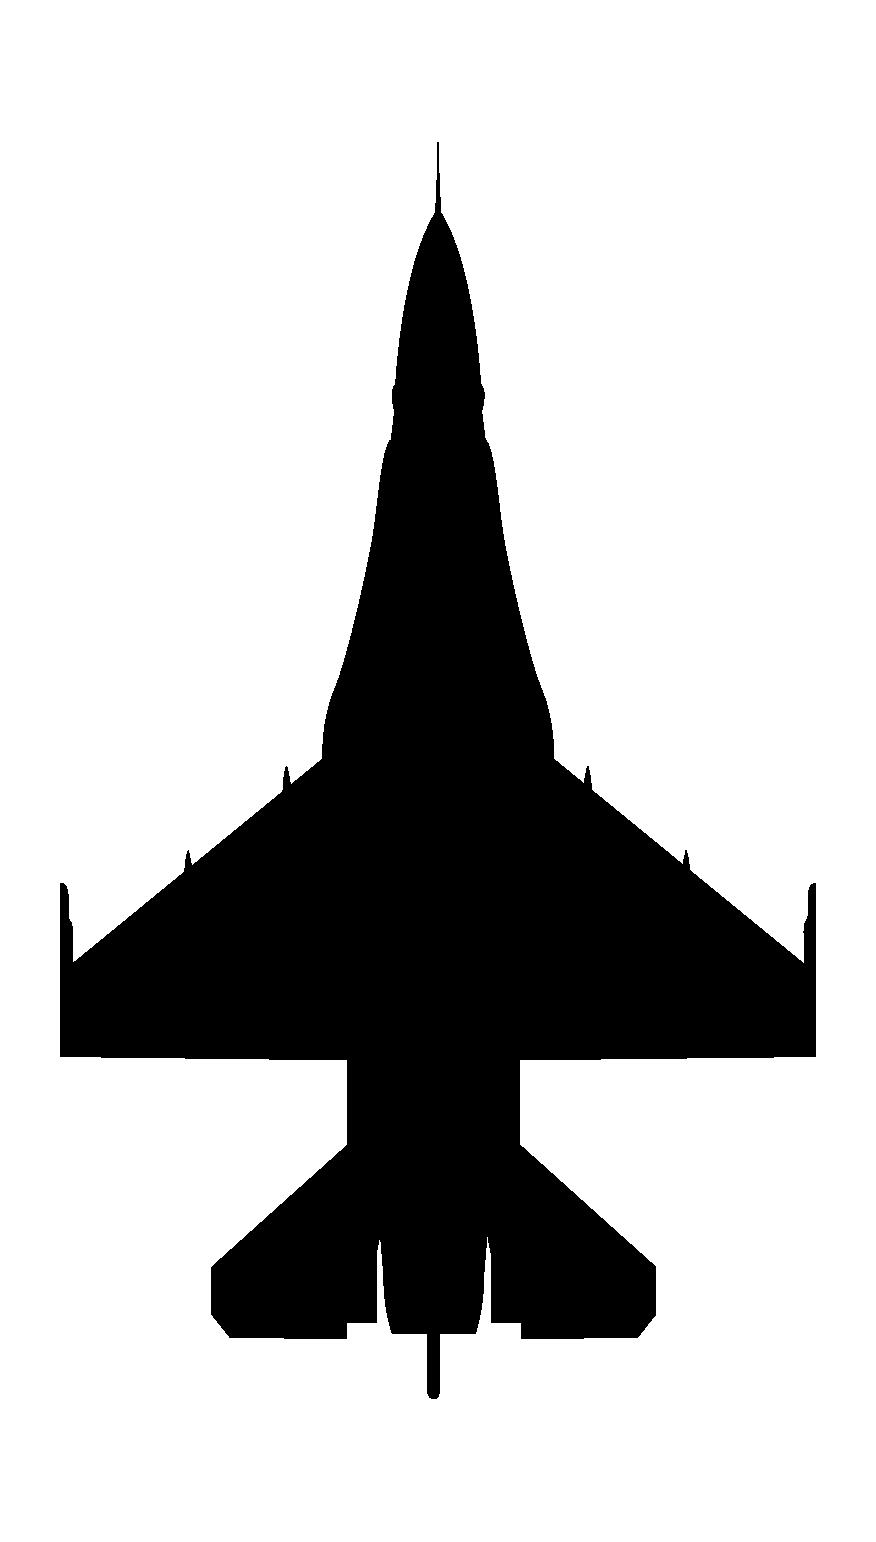
\includegraphics[
                width=7.5mm,
            ]{diagrams/aircraft/silhouette_f16_top.pdf}} 
            ++(0,20) 
            arc (180:90:10) 
            -- ++(10,0) 
            node[above, pos=1, rotate=-90]{
                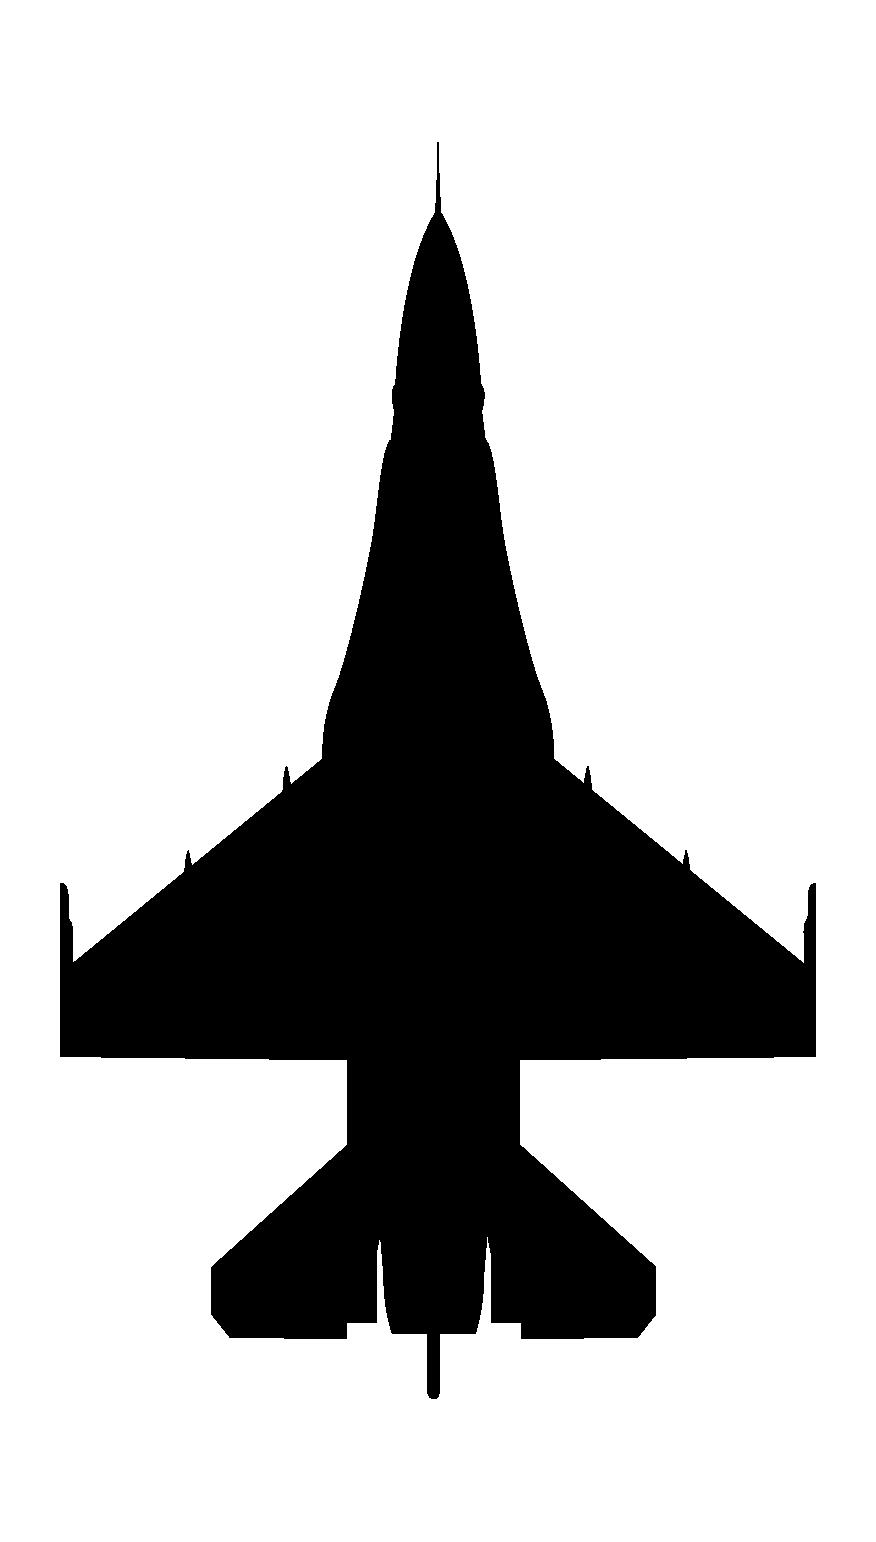
\includegraphics[
                    width=7.5mm,
            ]{diagrams/aircraft/silhouette_f16_top.pdf}};
        \end{tikzpicture}
        \caption{90 right}
    \end{subfigure}
    \begin{subfigure}[b]{0.45\linewidth}
        \centering
        \begin{tikzpicture}[figstyle]
            
            \draw[->] 
            (0,0) -- 
            node[below, pos=0]{
                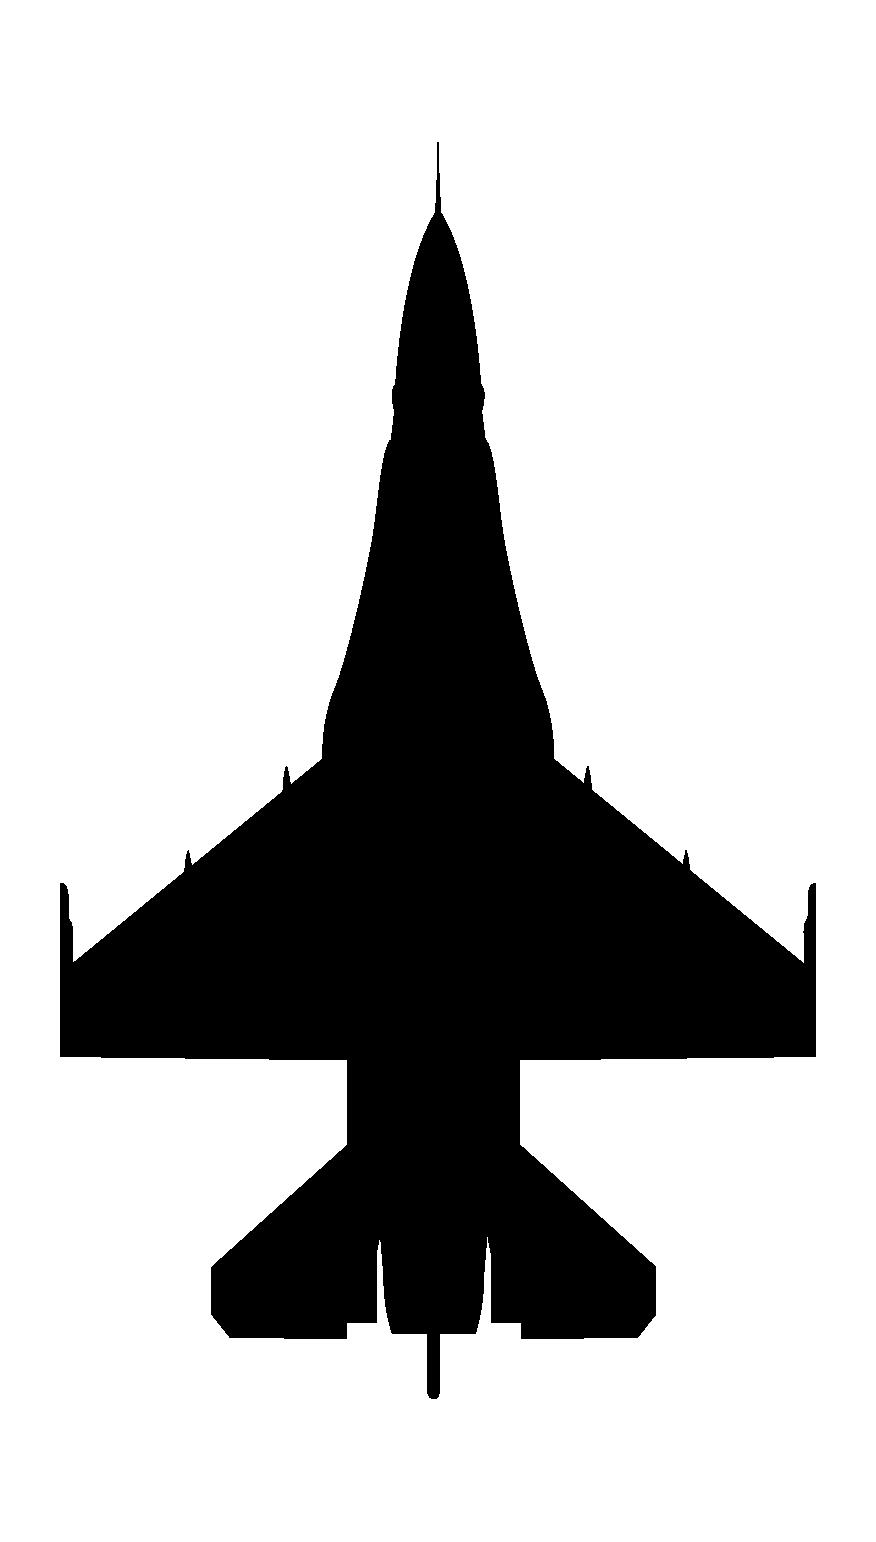
\includegraphics[
                width=7.5mm,
            ]{diagrams/aircraft/silhouette_f16_top.pdf}} 
            ++(0,27.5) 
            arc (0:45:10)  
            -- ++(-5,5) 
            node[above, pos=1, rotate=45]{
                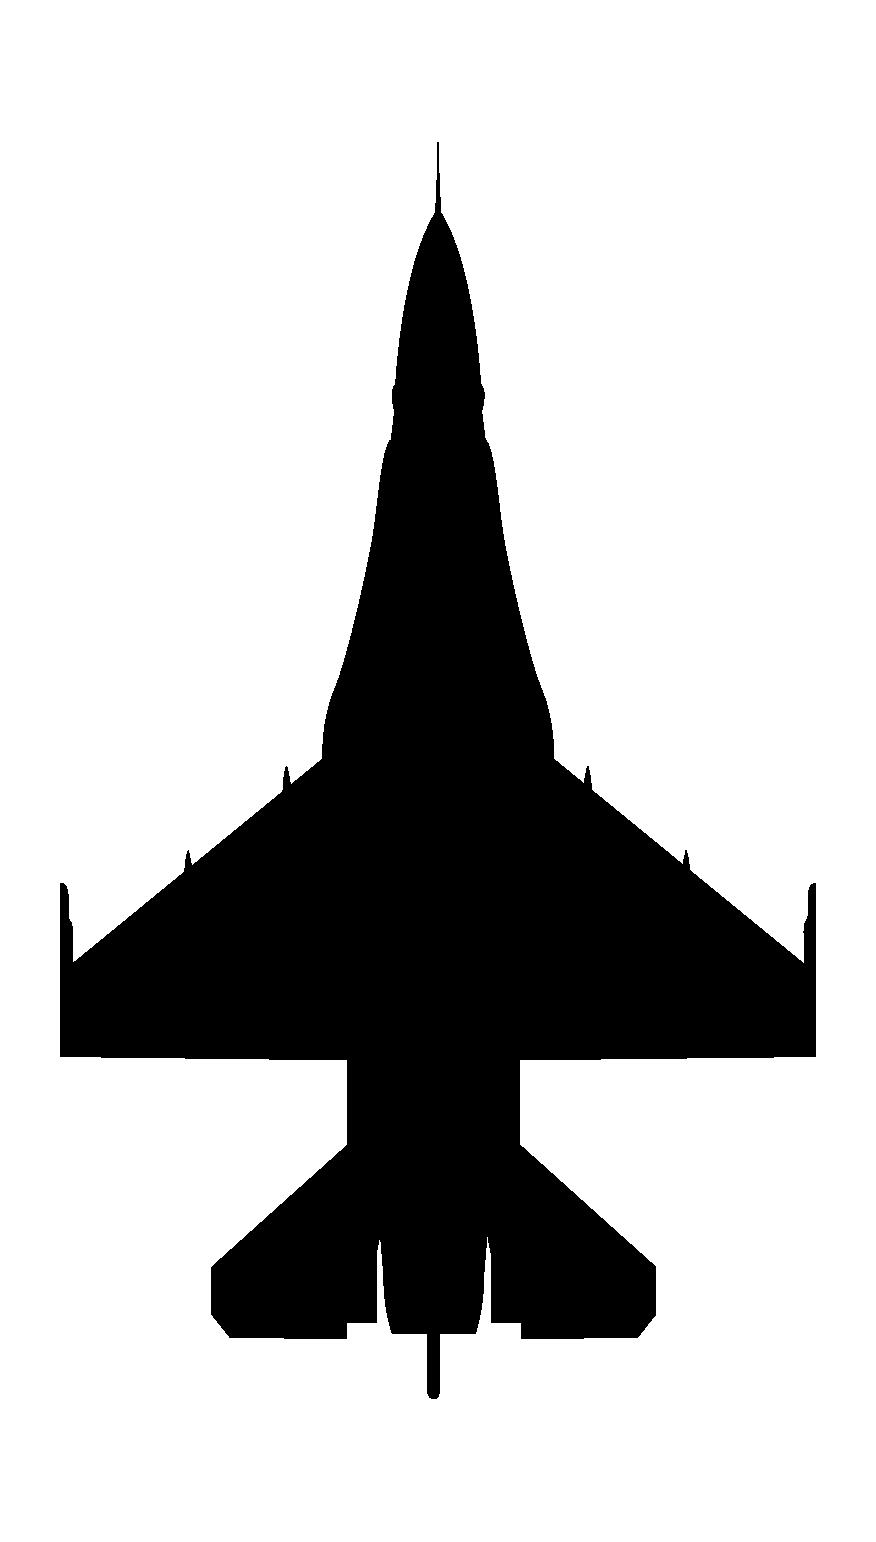
\includegraphics[
                    width=7.5mm,
            ]{diagrams/aircraft/silhouette_f16_top.pdf}};
                
            \draw[->] 
            (10,0) -- 
            node[below, pos=0]{
                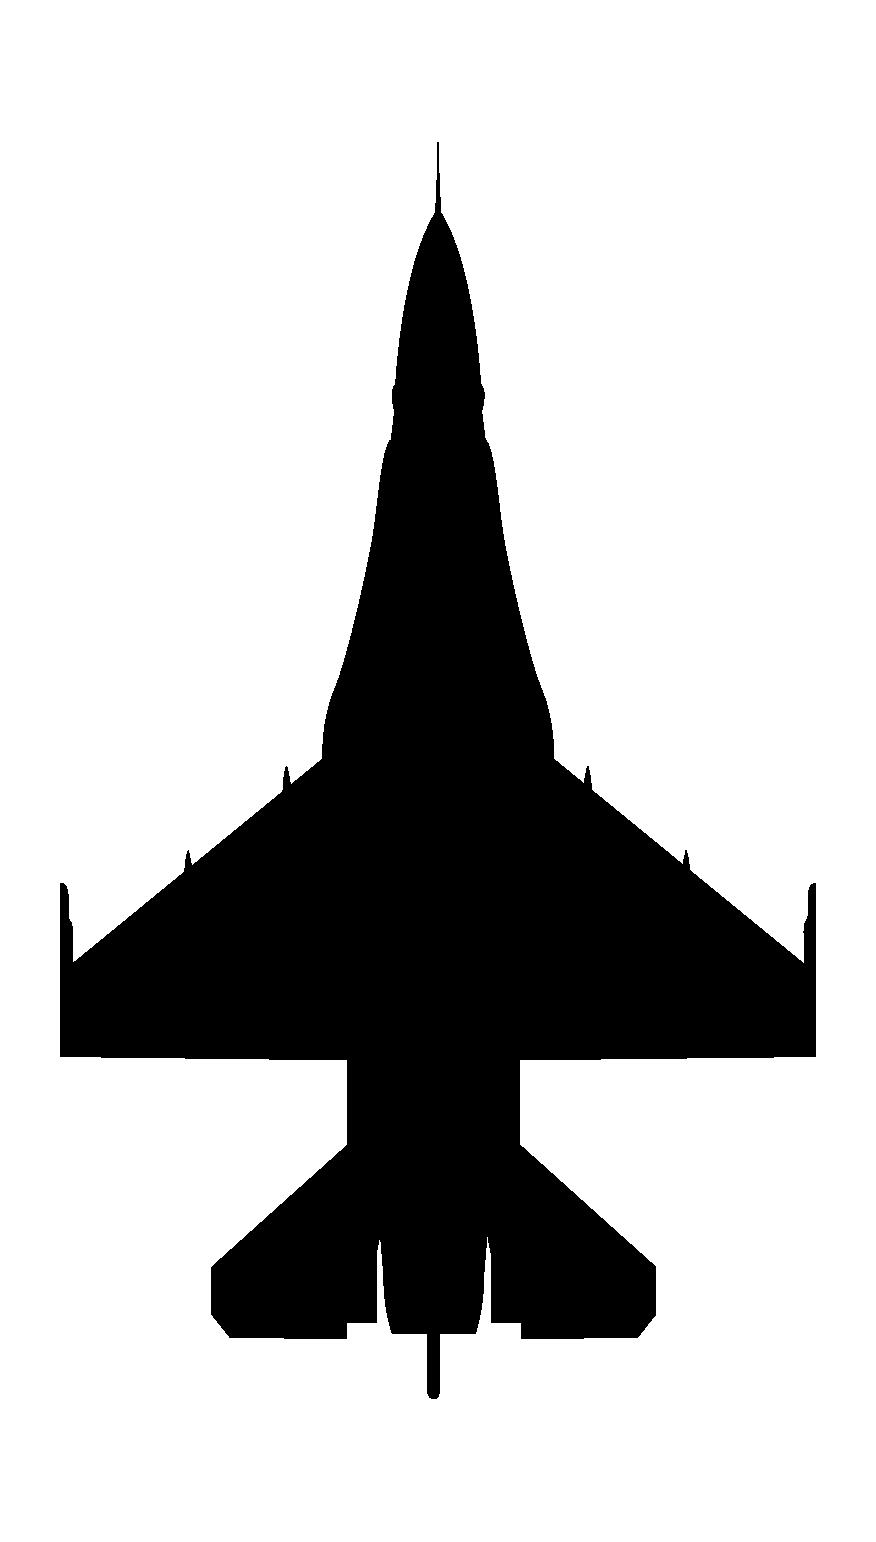
\includegraphics[
                width=7.5mm,
            ]{diagrams/aircraft/silhouette_f16_top.pdf}} 
            ++(0,2.5) 
            arc (0:45:10) 
            -- ++(-22.5,22.5) 
            node[above, pos=1, rotate=45]{
                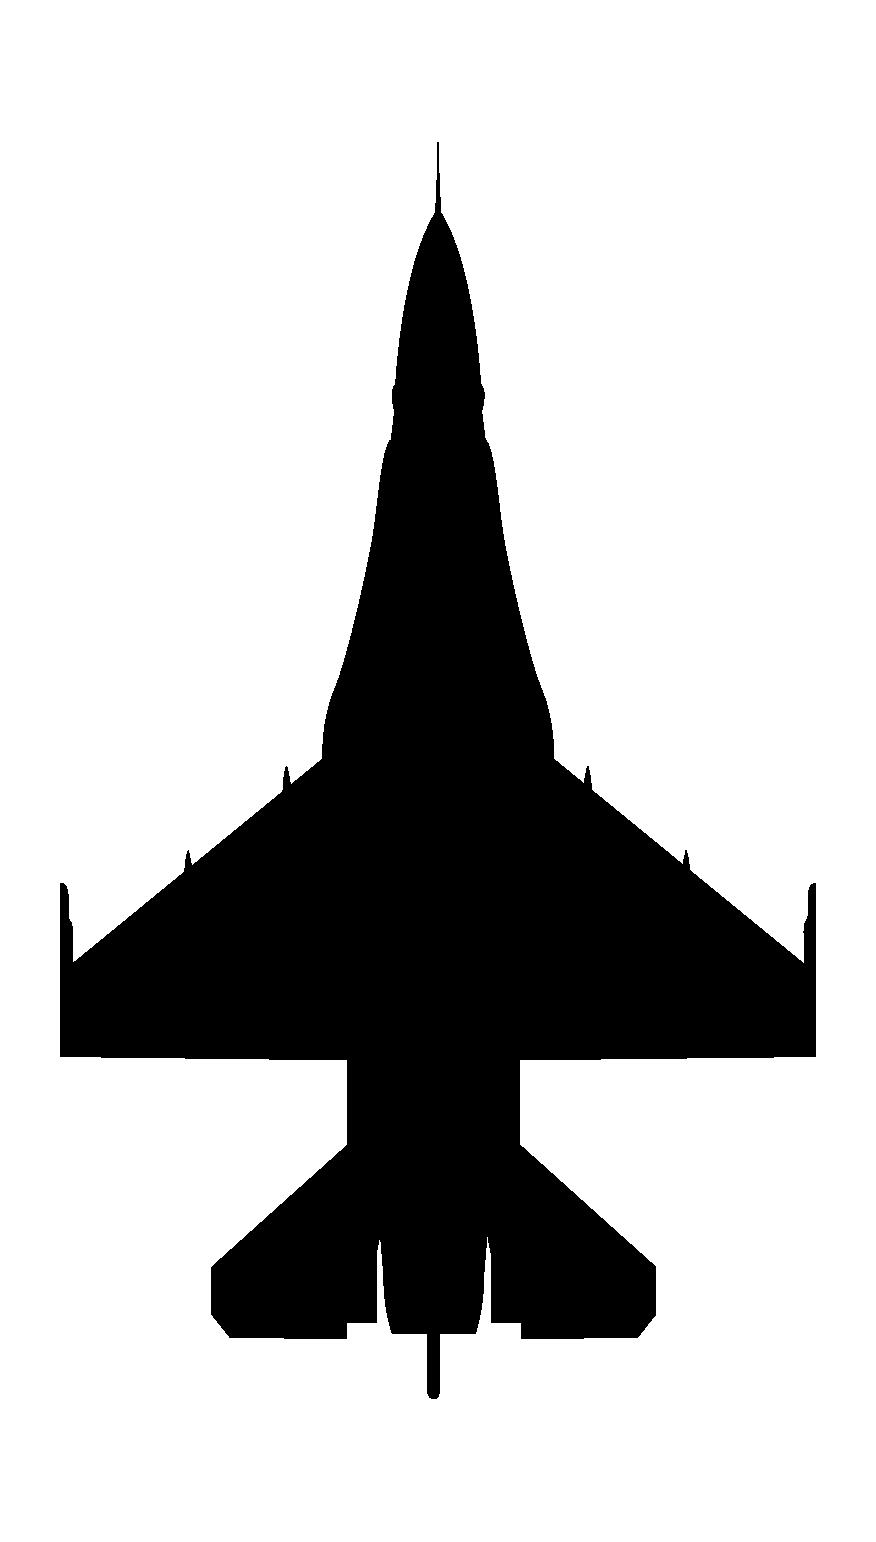
\includegraphics[
                    width=7.5mm,
            ]{diagrams/aircraft/silhouette_f16_top.pdf}};
    
        \end{tikzpicture}
        \caption{45 left}
    \end{subfigure}
    \caption{Tactical turn}
    \label{fig:supp_fig:form:tacturn}
\end{figure}

\begin{figure}[htbp]
    \centering
    \begin{tikzpicture}[figstyle]
            
        \draw[->] 
        (0,0) -- 
        node[below, pos=0]{
            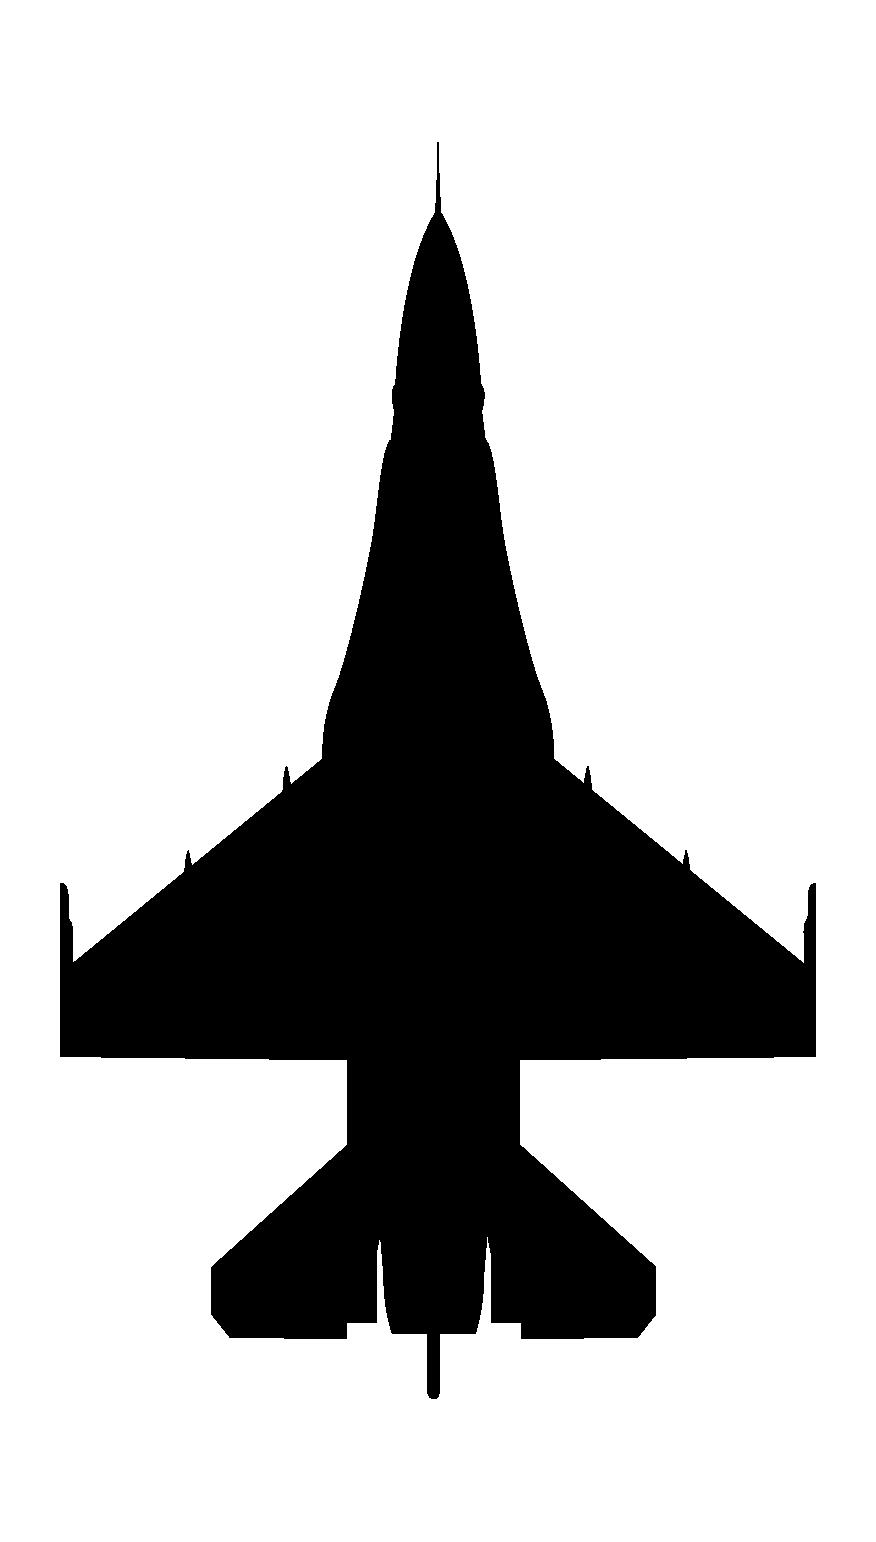
\includegraphics[
            width=7.5mm,
        ]{diagrams/aircraft/silhouette_f16_top.pdf}} 
        ++(0,20) 
        arc (180:00:10) 
        -- ++(0,-10)
        node[above, pos=1, rotate=180]{
            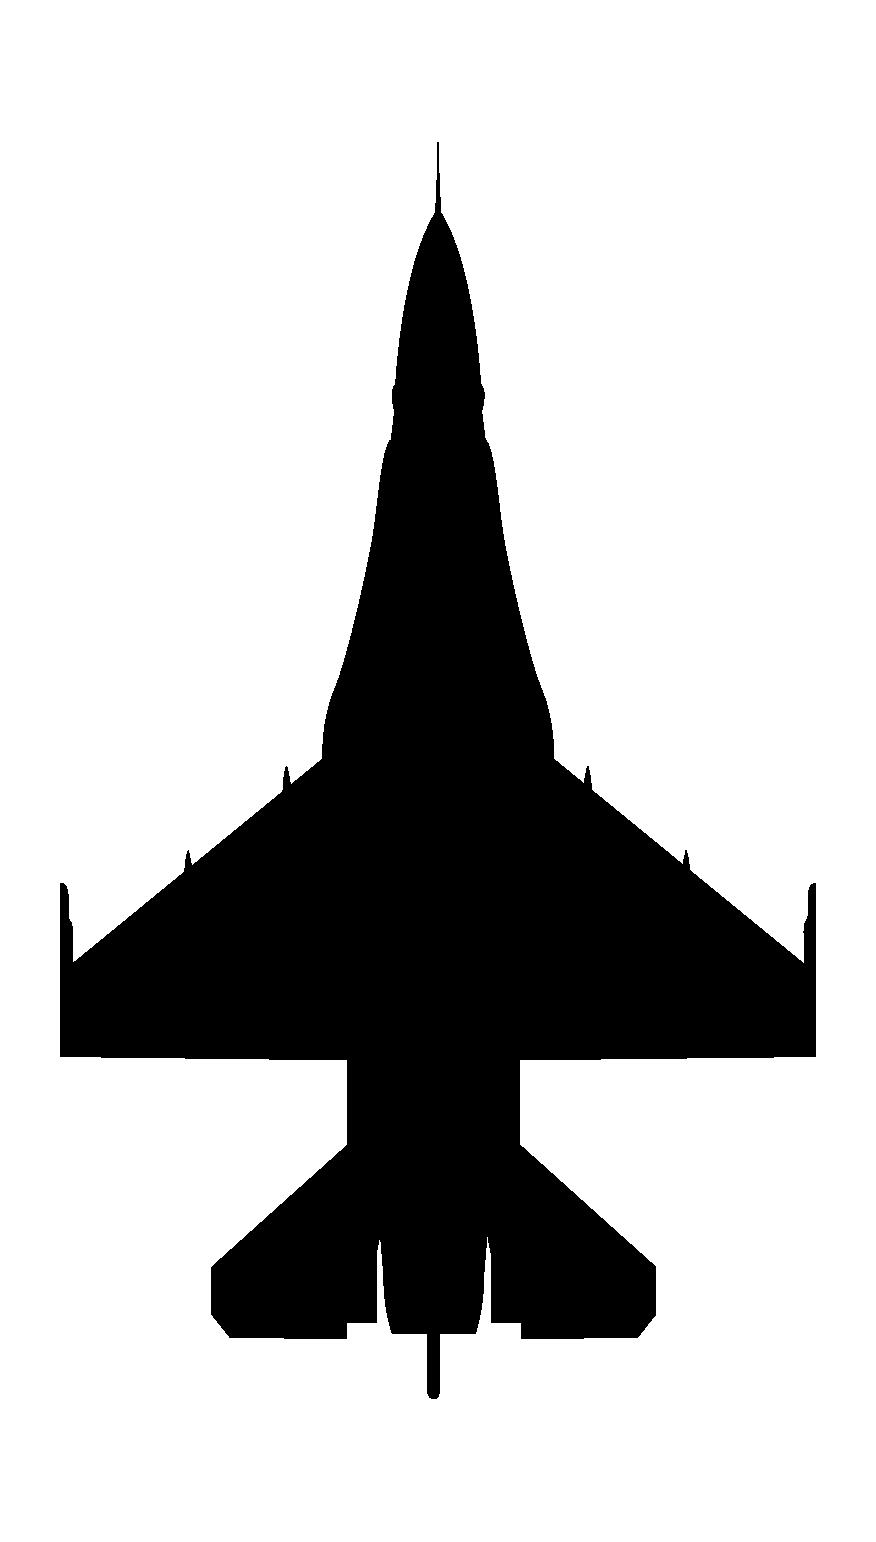
\includegraphics[
                width=7.5mm,
        ]{diagrams/aircraft/silhouette_f16_top.pdf}};
            
        \draw[->] 
        (10,0) -- 
        node[below, pos=0]{
            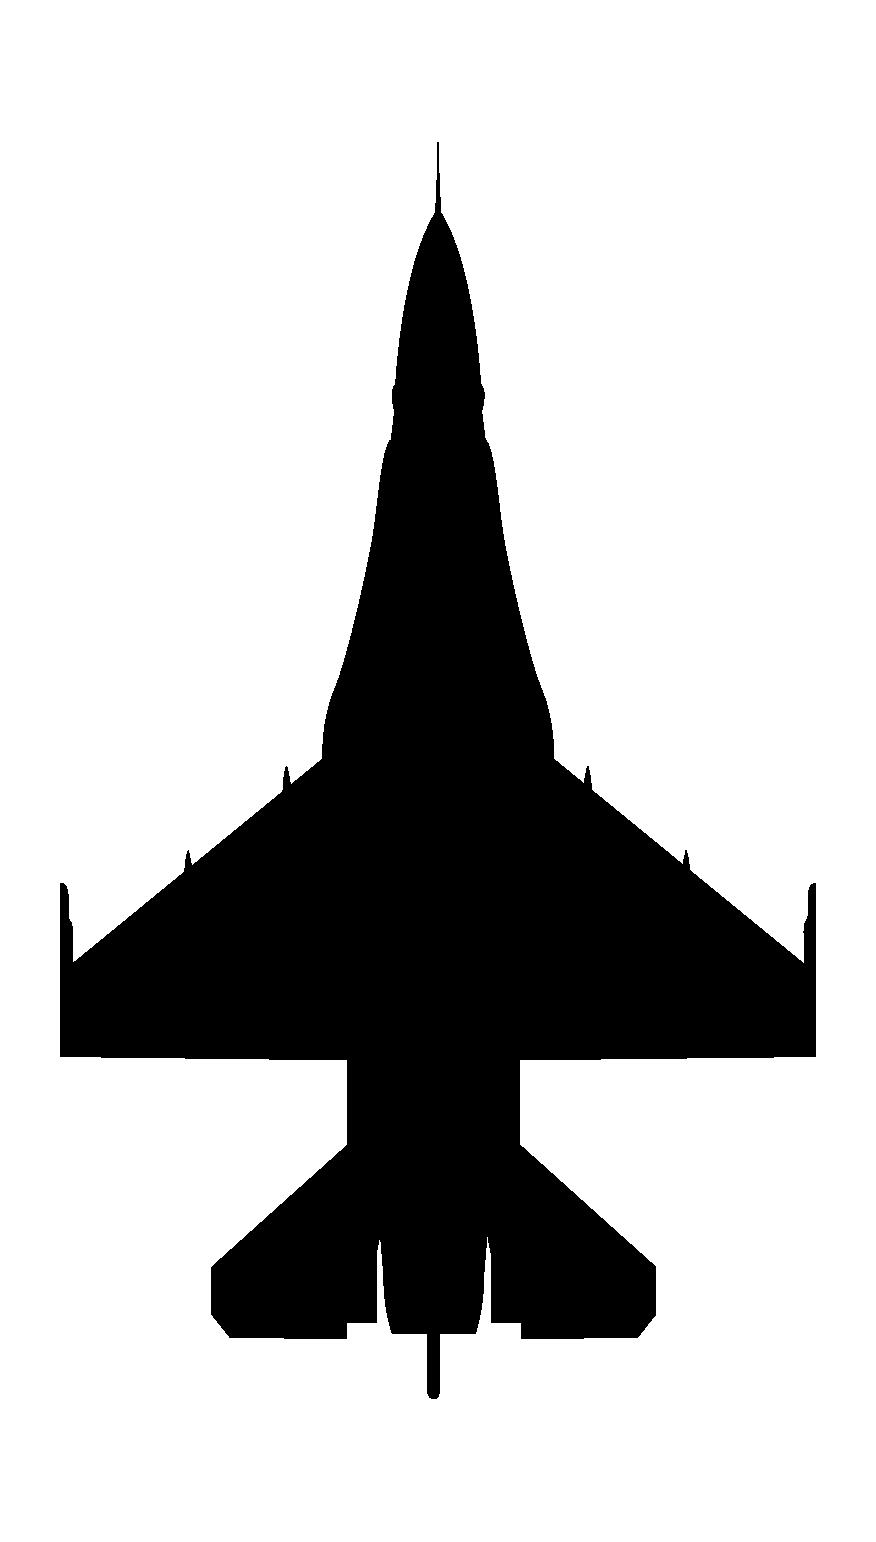
\includegraphics[
            width=7.5mm,
        ]{diagrams/aircraft/silhouette_f16_top.pdf}} 
        ++(0,20) 
        arc (180:0:10) 
        -- ++(0,-10)
        node[above, pos=1, rotate=180]{
            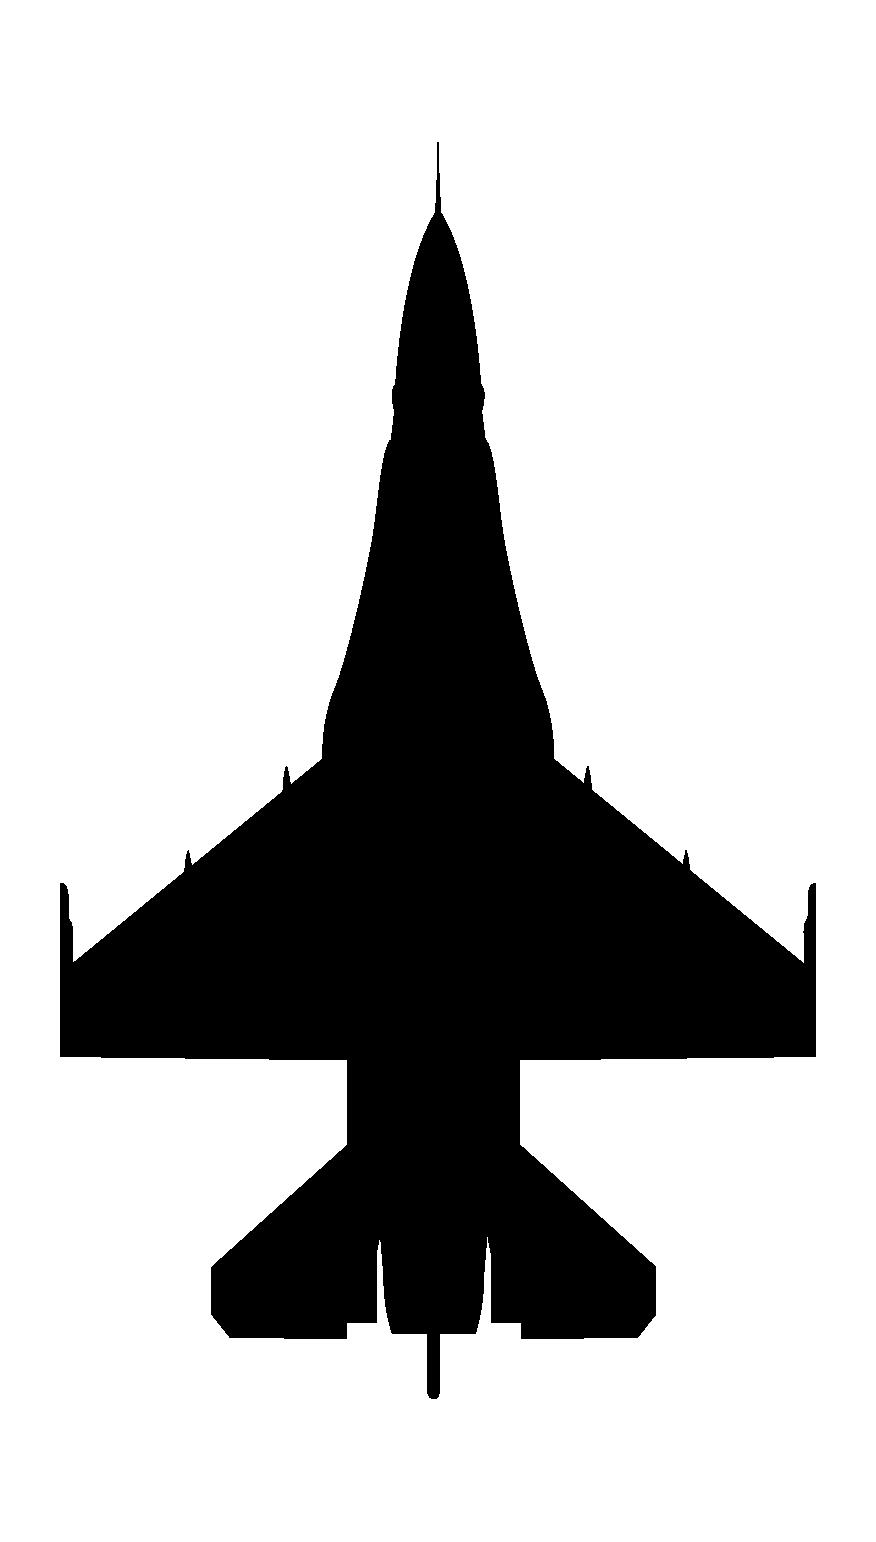
\includegraphics[
                width=7.5mm,
        ]{diagrams/aircraft/silhouette_f16_top.pdf}};

    \end{tikzpicture}
    \caption{Hook turn}
    \label{fig:supp_fig:form:hookturn}
\end{figure}

\begin{figure}[htbp]
    \centering
    \begin{tikzpicture}[figstyle]
            
        \draw[->] 
        (0,0) -- 
        node[below, pos=0]{
            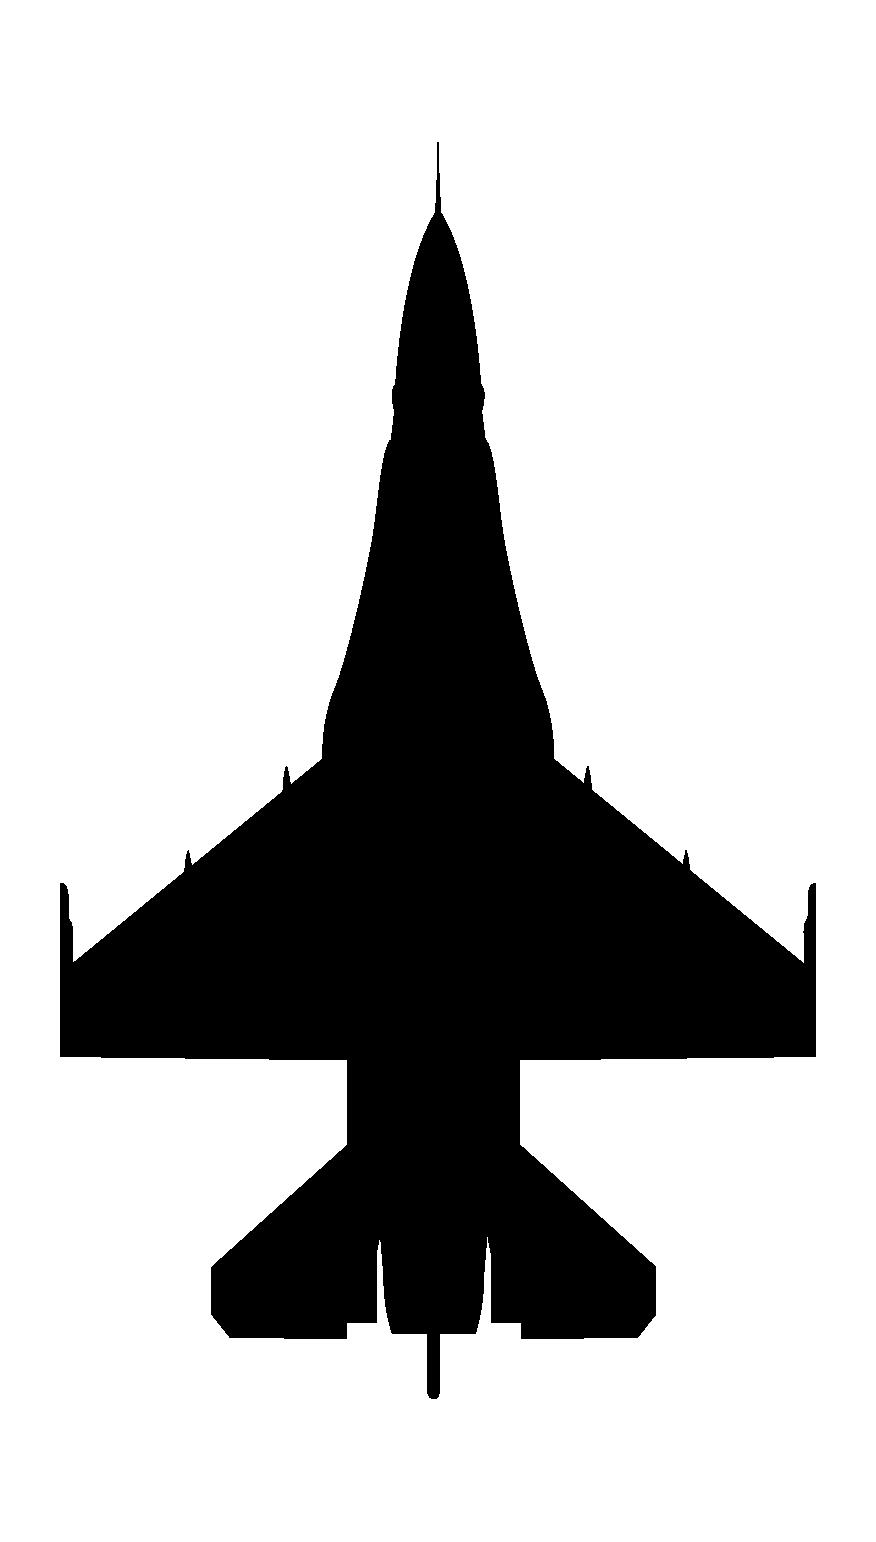
\includegraphics[
            width=7.5mm,
        ]{diagrams/aircraft/silhouette_f16_top.pdf}} 
        ++(0,20) 
        arc (180:00:10) 
        -- ++(0,-10)
        node[above, pos=1, rotate=180]{
            \includegraphics[
                width=7.5mm,
        ]{diagrams/aircraft/silhouette_f16_top.pdf}};
            
        \draw[->] 
        (10,0) -- 
        node[below, pos=0]{
            \includegraphics[
            width=7.5mm,
        ]{diagrams/aircraft/silhouette_f16_top.pdf}} 
        ++(0,20) 
        arc (0:180:10) 
        -- ++(0,-10)
        node[above, pos=1, rotate=180]{
            \includegraphics[
                width=7.5mm,
        ]{diagrams/aircraft/silhouette_f16_top.pdf}};

    \end{tikzpicture}
    \caption{Cross turn}
    \label{fig:supp_fig:form:crossturn}
\end{figure}

\begin{figure}[htbp]
    \centering
    \begin{tikzpicture}[figstyle]
            
        \draw[->] 
        (0,0) -- 
        node[below, pos=0]{
            \includegraphics[
            width=7.5mm,
        ]{diagrams/aircraft/silhouette_f16_top.pdf}} 
        ++(0,5) 
        arc (180:135:17) 
        arc (-45:0:17) 
        -- ++(0,5)
        node[above, pos=1]{
            \includegraphics[
                width=7.5mm,
        ]{diagrams/aircraft/silhouette_f16_top.pdf}};
            
        \draw[->] 
        (10,0) -- 
        node[below, pos=0]{
            \includegraphics[
            width=7.5mm,
        ]{diagrams/aircraft/silhouette_f16_top.pdf}} 
        ++(0,5) 
        arc (0:45:17) 
        arc (-135:-180:17) 
        -- ++(0,5)
        node[above, pos=1]{
            \includegraphics[
                width=7.5mm,
        ]{diagrams/aircraft/silhouette_f16_top.pdf}};

    \end{tikzpicture}
    \caption{Shackle}
    \label{fig:supp_fig:form:shackle}
\end{figure}

\cleardoublepage